% Paper 3 of the fBm series.  Compile:  xelatex main && bibtex main && xelatex main && xelatex main
% (TeX Live 2025; TEXMFVAR/TEXMFCACHE/TEXMFCONFIG redirected to work/.texmf_var -- see code/manuscript/build.ps1)
\documentclass[final,3p,11pt]{elsarticle}
\usepackage{mathtools}
\usepackage{amsthm}   % amsmath (via mathtools) first, then amsthm, then unicode-math (p3fonts); no amssymb
% p3fonts.tex -- the ONE font set-up shared by the manuscript and by every figure (matplotlib PGF backend, XeLaTeX).
% Latin Modern text with optical sizes (as lmodern does under pdfLaTeX) and Latin Modern Math via unicode-math.
% Fonts are loaded by file name (kpathsea), so no system font cache is consulted or written.
\usepackage{amsmath}
\usepackage{fontspec}
\defaultfontfeatures{Ligatures=TeX}
\setmainfont{lmroman10-regular.otf}[
  UprightFeatures = {SizeFeatures = {
      {Size = -5.5,      Font = lmroman5-regular.otf},
      {Size = 5.5-6.5,   Font = lmroman6-regular.otf},
      {Size = 6.5-7.5,   Font = lmroman7-regular.otf},
      {Size = 7.5-8.5,   Font = lmroman8-regular.otf},
      {Size = 8.5-9.5,   Font = lmroman9-regular.otf},
      {Size = 9.5-11.5,  Font = lmroman10-regular.otf},
      {Size = 11.5-14.5, Font = lmroman12-regular.otf},
      {Size = 14.5-,     Font = lmroman17-regular.otf}}},
  BoldFont = lmroman10-bold.otf,
  BoldFeatures = {SizeFeatures = {
      {Size = -5.5,      Font = lmroman5-bold.otf},
      {Size = 5.5-6.5,   Font = lmroman6-bold.otf},
      {Size = 6.5-7.5,   Font = lmroman7-bold.otf},
      {Size = 7.5-8.5,   Font = lmroman8-bold.otf},
      {Size = 8.5-9.5,   Font = lmroman9-bold.otf},
      {Size = 9.5-11.5,  Font = lmroman10-bold.otf},
      {Size = 11.5-,     Font = lmroman12-bold.otf}}},
  ItalicFont = lmroman10-italic.otf,
  ItalicFeatures = {SizeFeatures = {
      {Size = -7.5,      Font = lmroman7-italic.otf},
      {Size = 7.5-8.5,   Font = lmroman8-italic.otf},
      {Size = 8.5-9.5,   Font = lmroman9-italic.otf},
      {Size = 9.5-11.5,  Font = lmroman10-italic.otf},
      {Size = 11.5-,     Font = lmroman12-italic.otf}}},
  BoldItalicFont = lmroman10-bolditalic.otf]
\setsansfont{lmsans10-regular.otf}[BoldFont = lmsans10-bold.otf, ItalicFont = lmsans10-oblique.otf]
\setmonofont{lmmono10-regular.otf}
\usepackage{unicode-math}
\setmathfont{latinmodern-math.otf}
\setmathfont{latinmodern-math.otf}[version=bold, FakeBold=2]   % bold headings with math (no bold Latin Modern Math exists)

\usepackage{booktabs,array,multirow,makecell,longtable}
\setcounter{LTchunksize}{1000}   % each longtable set in one chunk: column widths correct in every LaTeX pass
\usepackage{graphicx}
\usepackage{xcolor}
\usepackage[font=small,labelfont=bf,skip=5pt]{caption}
\usepackage{microtype}
\usepackage[colorlinks=true,linkcolor=blue!50!black,citecolor=blue!50!black,urlcolor=blue!50!black]{hyperref}
\usepackage[capitalise,nameinlink]{cleveref}
\hypersetup{pdftitle={CosCert: certified critical values and exact size for long-memory tests of the mean},
  pdfauthor={Eslam Ahmed, Mohamed A. El-Beltagy, Ahmed Etman, Sroor M. Elnady}}
\graphicspath{{../figures/}}
\setlength{\emergencystretch}{2em}   % prefer slightly looser lines to overfull ones
% elsarticle puts "Appendix" into \thesection: print appendix references as the bare number
\crefformat{appendix}{#2#1#3}\Crefformat{appendix}{#2#1#3}
\crefmultiformat{appendix}{#2#1#3}{ and~#2#1#3}{, #2#1#3}{ and~#2#1#3}
\Crefmultiformat{appendix}{#2#1#3}{ and~#2#1#3}{, #2#1#3}{ and~#2#1#3}
\crefrangeformat{appendix}{#3#1#4 to~#5#2#6}
\journal{Computational Statistics \& Data Analysis}

% ---------------------------------------------------------------- traceable numbers
% Every reported number is \pthree{<key>}; keys are written by code/manuscript/make_numbers.py from work/results.
\makeatletter
\newcommand{\pthreedef}[2]{\expandafter\def\csname p3@#1\endcsname{#2}}
\newcommand{\pthree}[1]{\ifcsname p3@#1\endcsname\csname p3@#1\endcsname\else
  \PackageError{p3numbers}{Undefined number key '#1'}{Run make_numbers.py}\textbf{??#1??}\fi}
\makeatother
% generated by code/manuscript/make_numbers.py -- do not edit
\pthreedef{arfima-trunc}{$1\times10^{-18}$}
\pthreedef{audit-D-hi0-jointz}{3.5}
\pthreedef{audit-D-hi0-max}{4.97}
\pthreedef{audit-D-hi0-maxz}{1.6}
\pthreedef{audit-D-hi0-min}{4.65}
\pthreedef{audit-D-hi0-n}{16}
\pthreedef{audit-D-hi0-rowz}{0.9}
\pthreedef{audit-D-jointz}{5.6}
\pthreedef{audit-D-jointz-rows}{2.8}
\pthreedef{audit-D-nrows}{4}
\pthreedef{audit-apkv-maxrel}{$7.9\times10^{-5}$}
\pthreedef{audit-hi-2se}{0.44}
\pthreedef{audit-hi-disc-max}{$2.0\times10^{0}$}
\pthreedef{audit-hi-neg-design-gt2}{3}
\pthreedef{audit-hi-neg-design-gt3}{0}
\pthreedef{audit-hi-neg-design-max}{5.45}
\pthreedef{audit-hi-neg-design-maxz}{2.08}
\pthreedef{audit-hi-neg-design-min}{4.56}
\pthreedef{audit-hi-neg-gt2se}{29}
\pthreedef{audit-hi-neg-gt3se}{28}
\pthreedef{audit-hi-neg-m1-limit}{3.1}
\pthreedef{audit-hi-neg-m16-T1e3}{3.9}
\pthreedef{audit-hi-neg-m16-T1e4}{5.5}
\pthreedef{audit-hi-neg-m16-T1e5}{7.0}
\pthreedef{audit-hi-neg-m16-fgn}{27.5}
\pthreedef{audit-hi-neg-m16-limit}{29.5}
\pthreedef{audit-hi-neg-max}{29.53}
\pthreedef{audit-hi-neg-maxdev}{24.5}
\pthreedef{audit-hi-neg-maxz}{113}
\pthreedef{audit-hi-neg-min}{3.13}
\pthreedef{audit-hi-neg-n}{80}
\pthreedef{audit-hi-pos-gt01}{58}
\pthreedef{audit-hi-pos-max}{5.34}
\pthreedef{audit-hi-pos-min}{4.65}
\pthreedef{audit-hi-pos-n}{96}
\pthreedef{audit-kpss-tau-05}{5.23}
\pthreedef{audit-kpss-tau-05-exact}{0.1479}
\pthreedef{audit-kpss-tau-05-z}{2.4}
\pthreedef{audit-kpsstau-jointz}{2.5}
\pthreedef{audit-lob-jointz}{1.7}
\pthreedef{audit-lob-sizes}{10.010, 5.023, 2.535, 1.015, 0.525}
\pthreedef{audit-mp-H090-a10}{10.31}
\pthreedef{audit-mp-T1-devmax}{-0.17}
\pthreedef{audit-mp-T1-devmin}{-0.46}
\pthreedef{audit-mp-T1-maxz}{3.8}
\pthreedef{audit-mp-T1-minz}{3.4}
\pthreedef{audit-mp-T3-dev10}{-2.85}
\pthreedef{audit-mp-T3-maxz}{28}
\pthreedef{audit-mp-T3-round-maxshift}{0.05}
\pthreedef{audit-mp-T3-round-mindev}{0.95}
\pthreedef{audit-mp-T3-size05}{2.33}
\pthreedef{audit-mp-neg-max}{-0.02}
\pthreedef{audit-mp-neg-min}{-2.85}
\pthreedef{audit-mp-pos-max}{0.31}
\pthreedef{audit-mp-pos-maxz}{2.94}
\pthreedef{audit-mp-pos-min}{0.03}
\pthreedef{audit-mp-pos-n}{16}
\pthreedef{audit-mp-pos-npos}{16}
\pthreedef{audit-n-A}{83}
\pthreedef{audit-n-AB}{165}
\pthreedef{audit-n-B}{82}
\pthreedef{audit-n-C}{28}
\pthreedef{audit-n-D}{32}
\pthreedef{audit-n-E}{8}
\pthreedef{audit-n-dup}{8}
\pthreedef{audit-n-entries}{241}
\pthreedef{audit-n-sources}{6}
\pthreedef{audit-n-values}{233}
\pthreedef{audit-n-within3}{189}
\pthreedef{bw-50-max-100}{22.3}
\pthreedef{bw-50-max-2000}{12.0}
\pthreedef{bw-50-min-100}{7.2}
\pthreedef{bw-50-min-2000}{5.9}
\pthreedef{bw-65-max-100}{17.8}
\pthreedef{bw-65-max-2000}{7.9}
\pthreedef{bw-65-min-100}{6.6}
\pthreedef{bw-65-min-2000}{5.3}
\pthreedef{bw-80-arfima0-max-500}{9.9}
\pthreedef{bw-80-fgn-maxdev-500}{0.7}
\pthreedef{bw-80-max-100}{16.5}
\pthreedef{bw-80-max-2000}{7.0}
\pthreedef{bw-80-min-100}{5.5}
\pthreedef{bw-80-min-2000}{4.4}
\pthreedef{clip-max}{one}
\pthreedef{clip-ncells}{120}
\pthreedef{clip-nwith}{67}
\pthreedef{clip-rel}{$9\times10^{-17}$}
\pthreedef{dominance-ncells}{120}
\pthreedef{dominance-share}{89}
\pthreedef{e1-slope-maxdev}{0.05}
\pthreedef{e1-tilt-node-ratio-max}{17}
\pthreedef{e1-tilt-node-ratio-min}{1.8}
\pthreedef{e1-width-max-16384}{$1.9\times10^{-6}$}
\pthreedef{e11-n-cat}{6}
\pthreedef{e11-n-rows}{19}
\pthreedef{e2r-maxchange}{$3\times10^{-15}$}
\pthreedef{e2r-n-brackets}{300}
\pthreedef{e2r-n-ok}{300}
\pthreedef{e5-3mom-T1-pp}{1.2}
\pthreedef{e5-T12-cert-s}{0.04}
\pthreedef{e5-T12-cert-width}{$8\times10^{-16}$}
\pthreedef{e5-T12-exact-maxerr}{$4\times10^{-11}$}
\pthreedef{e5-T12-exact-maxs}{$9\times10^{-3}$}
\pthreedef{e5-T3-eig-s}{0.31}
\pthreedef{e5-T3-ifft-s}{975}
\pthreedef{e5-T3-imhof-s}{0.32}
\pthreedef{e5-T3-query-s}{0.06}
\pthreedef{e5-T3-setup-s}{0.37}
\pthreedef{e5-T4-cert-eval-s}{15.7}
\pthreedef{e5-T4-cert-s}{40.5}
\pthreedef{e5-T4-galerkin-err}{$9.5\times10^{-9}$}
\pthreedef{e5-T4-galerkin-s}{0.3}
\pthreedef{e5-T4-ray2048-s}{3049}
\pthreedef{e5-T4-ref-width}{$1.9\times10^{-8}$}
\pthreedef{e5-amort-imhof-s}{4.0}
\pthreedef{e5-amort-m}{10}
\pthreedef{e5-amort-maxdiff}{$6\times10^{-14}$}
\pthreedef{e5-amort-ours-s}{1.1}
\pthreedef{e5-amort-ratio}{3.6}
\pthreedef{e5-approx-maxerr-pp}{5.0}
\pthreedef{e5-env}{12 logical CPUs, Windows 10, Python 3.12.14, R 4.5.3}
\pthreedef{e5-gh-maxdiff-pp}{0.08}
\pthreedef{e5-hbe-err-pp}{1.17}
\pthreedef{e5-lead20-err}{$1.5\times10^{-8}$}
\pthreedef{e5-lpb4-err-pp}{0.23}
\pthreedef{e5-lr-err-pp}{0.88}
\pthreedef{e5-ltz-T1-pp}{1.2}
\pthreedef{e5-n-fail}{4}
\pthreedef{e5-n-impl}{21}
\pthreedef{e5-n-methods}{14}
\pthreedef{e5-n-targets-rows}{92}
\pthreedef{e5-satt-err-pp}{4.6}
\pthreedef{e5-svsaddle-err-pp}{0.19}
\pthreedef{edge-C-0.900}{38.86}
\pthreedef{edge-C-0.950}{69.76}
\pthreedef{edge-C-0.990}{191.0}
\pthreedef{edge-extrap-maxrel}{0.07}
\pthreedef{edge-mu1-share}{81}
\pthreedef{edge-rho-min}{0.23}
\pthreedef{fgn-sn-0.70-500-dev}{$2.4\times10^{-5}$}
\pthreedef{fn-arfima1m-HI16-0.50-50}{1.9}
\pthreedef{fn-arfima1p-HI1-0.50-50}{5.1}
\pthreedef{fn-arfima1p-HI16-0.50-50}{19.1}
\pthreedef{fn-arfima1p-HI16-0.90-50}{12.0}
\pthreedef{fn-arfima1p-HI4-0.70-100}{5.5}
\pthreedef{fn-arfima1p-SN-0.50-50}{7.2}
\pthreedef{fn-arfima1p-SN-0.70-100}{5.5}
\pthreedef{fn-maxdev-2000}{0.05}
\pthreedef{fn-maxdev-pure}{0.54}
\pthreedef{fn-maxdev-small-100}{0.56}
\pthreedef{fx-n-cells}{3\,900}
\pthreedef{g0-max-digits}{15}
\pthreedef{g0-min-digits}{14}
\pthreedef{hi17-R}{100\,000}
\pthreedef{hi17-T5-64-16-plugin}{22.6}
\pthreedef{hi17-maxdiff}{2.0}
\pthreedef{hi17-meandiff}{+0.19}
\pthreedef{hi17-ncells}{144}
\pthreedef{hi17-share-z2}{35}
\pthreedef{hi17-t2-maxz}{2.17}
\pthreedef{hi17-t2-n}{64}
\pthreedef{ledger-n-cv}{245}
\pthreedef{ledger-n-rr}{317}
\pthreedef{mx-0.50-128}{5.0042}
\pthreedef{mx-0.50-64}{5.0167}
\pthreedef{mx-0.90-128}{42.8081}
\pthreedef{mx-0.90-64}{42.8085}
\pthreedef{mx-0.99-128}{79.5227}
\pthreedef{mx-0.99-128-own}{5.00004}
\pthreedef{mx-0.99-128-round}{5.00008}
\pthreedef{mx-0.99-64}{79.5227}
\pthreedef{mx-cv-0.99}{6829.94}
\pthreedef{mx-gap-128}{$4.2\times10^{-3}$}
\pthreedef{mx-gap-128-H}{0.50}
\pthreedef{mx-gap-128-long}{$6.9\times10^{-5}$}
\pthreedef{mx-gap-64}{$1.7\times10^{-2}$}
\pthreedef{mx-gap-64-H}{0.50}
\pthreedef{mx-gap-64-long}{$4.9\times10^{-4}$}
\pthreedef{mx-maxdiff-AB}{$6.7\times10^{-12}$}
\pthreedef{mx-maxdiff-user}{$3.6\times10^{-5}$}
\pthreedef{naive-hi1-0.90}{26.2}
\pthreedef{naive-hi16-0.90}{71.3}
\pthreedef{naive-hi4-0.90}{55.2}
\pthreedef{naive-max-0.90}{71.3}
\pthreedef{naive-min-0.90}{25.6}
\pthreedef{naive-sn-0.70-0.05}{16.5}
\pthreedef{naive-sn-0.90-0.05}{42.8}
\pthreedef{or-inside-pct}{98.9}
\pthreedef{or-maxz}{3.82}
\pthreedef{or-n-cells}{1\,800}
\pthreedef{or-z-mean}{-0.09}
\pthreedef{or-z-sd}{0.99}
\pthreedef{pl-HI4-H05-trunc}{4.6}
\pthreedef{pl-HI4-H05-untrunc}{9.5}
\pthreedef{pl-R}{40\,000}
\pthreedef{pl-ar1m-max-100}{23.5}
\pthreedef{pl-ar1p-max}{4.6}
\pthreedef{pl-ar1p-min}{1.9}
\pthreedef{pl-arfima0-HI16-0.7-100}{11.8}
\pthreedef{pl-arfima0-HI16-0.7-2000}{6.8}
\pthreedef{pl-arfima0-HI16-0.9-100}{17.8}
\pthreedef{pl-arfima0-HI16-0.9-2000}{7.9}
\pthreedef{pl-arfima0-HI4-0.7-100}{10.2}
\pthreedef{pl-arfima0-HI4-0.7-2000}{6.2}
\pthreedef{pl-arfima0-HI4-0.9-100}{15.8}
\pthreedef{pl-arfima0-HI4-0.9-2000}{7.2}
\pthreedef{pl-arfima0-SN-0.7-100}{9.0}
\pthreedef{pl-arfima0-SN-0.7-2000}{5.8}
\pthreedef{pl-arfima0-SN-0.9-100}{13.2}
\pthreedef{pl-arfima0-SN-0.9-2000}{6.4}
\pthreedef{pl-arfima1m-HI16-0.7-100}{14.5}
\pthreedef{pl-arfima1m-HI16-0.7-2000}{7.3}
\pthreedef{pl-arfima1m-HI16-0.9-100}{23.5}
\pthreedef{pl-arfima1m-HI16-0.9-2000}{9.0}
\pthreedef{pl-arfima1m-HI4-0.7-100}{12.3}
\pthreedef{pl-arfima1m-HI4-0.7-2000}{6.4}
\pthreedef{pl-arfima1m-HI4-0.9-100}{20.4}
\pthreedef{pl-arfima1m-HI4-0.9-2000}{8.2}
\pthreedef{pl-arfima1m-SN-0.7-100}{10.3}
\pthreedef{pl-arfima1m-SN-0.7-2000}{5.9}
\pthreedef{pl-arfima1m-SN-0.9-100}{16.4}
\pthreedef{pl-arfima1m-SN-0.9-2000}{7.0}
\pthreedef{pl-arfima1p-HI16-0.7-100}{3.1}
\pthreedef{pl-arfima1p-HI16-0.7-2000}{4.0}
\pthreedef{pl-arfima1p-HI16-0.9-100}{3.4}
\pthreedef{pl-arfima1p-HI16-0.9-2000}{3.7}
\pthreedef{pl-arfima1p-HI4-0.7-100}{3.2}
\pthreedef{pl-arfima1p-HI4-0.7-2000}{4.1}
\pthreedef{pl-arfima1p-HI4-0.9-100}{3.4}
\pthreedef{pl-arfima1p-HI4-0.9-2000}{3.7}
\pthreedef{pl-arfima1p-SN-0.7-100}{3.0}
\pthreedef{pl-arfima1p-SN-0.7-2000}{4.2}
\pthreedef{pl-arfima1p-SN-0.9-100}{3.1}
\pthreedef{pl-arfima1p-SN-0.9-2000}{3.5}
\pthreedef{pl-fgn-HI16-0.7-100}{11.1}
\pthreedef{pl-fgn-HI16-0.7-2000}{6.9}
\pthreedef{pl-fgn-HI16-0.9-100}{15.6}
\pthreedef{pl-fgn-HI16-0.9-2000}{7.8}
\pthreedef{pl-fgn-HI4-0.7-100}{9.7}
\pthreedef{pl-fgn-HI4-0.7-2000}{6.2}
\pthreedef{pl-fgn-HI4-0.9-100}{14.0}
\pthreedef{pl-fgn-HI4-0.9-2000}{7.2}
\pthreedef{pl-fgn-SN-0.7-100}{8.6}
\pthreedef{pl-fgn-SN-0.7-2000}{5.9}
\pthreedef{pl-fgn-SN-0.9-100}{11.8}
\pthreedef{pl-fgn-SN-0.9-2000}{6.5}
\pthreedef{pl-n-pure-cells}{40}
\pthreedef{pl-pure-max-100}{17.8}
\pthreedef{pl-pure-max-2000}{7.9}
\pthreedef{pl-pure-min-100}{5.5}
\pthreedef{pl-pure-min-2000}{5.2}
\pthreedef{pl-share-ewc4-le-sn}{65}
\pthreedef{pl-share-hi1-le-sn}{100}
\pthreedef{pl-share-sn-le-hi4}{100}
\pthreedef{pw-HI1-0.75}{0.354}
\pthreedef{pw-HI16-0.50}{0.775}
\pthreedef{pw-HI16-0.75}{0.770}
\pthreedef{pw-HI16-0.90}{0.758}
\pthreedef{pw-HI4-0.70}{0.687}
\pthreedef{pw-HI4-0.75}{0.685}
\pthreedef{pw-SN-0.50}{0.599}
\pthreedef{pw-SN-0.70}{0.542}
\pthreedef{pw-SN-0.90}{0.491}
\pthreedef{pw-c0-maxdev}{$1.3\times10^{-9}$}
\pthreedef{pw-hi-ewc-maxdiff}{0.002}
\pthreedef{pw-jl-128-512}{$8.0\times10^{-8}$}
\pthreedef{pw-jl-256-512}{$9.0\times10^{-9}$}
\pthreedef{pw-jl-512-1024}{$1.1\times10^{-9}$}
\pthreedef{pw-nct-maxdev}{$2.3\times10^{-13}$}
\pthreedef{pw-nct-ncells}{610}
\pthreedef{pw-vsSN-EWC2-min}{-0.288}
\pthreedef{pw-vsSN-EWC2-npos}{0}
\pthreedef{pw-vsSN-EWC4-min}{-0.037}
\pthreedef{pw-vsSN-EWC4-npos}{304}
\pthreedef{pw-vsSN-EWC8-min}{0.000}
\pthreedef{pw-vsSN-EWC8-npos}{360}
\pthreedef{pw-vsSN-HI1-min}{-0.288}
\pthreedef{pw-vsSN-HI1-npos}{0}
\pthreedef{pw-vsSN-HI2-min}{-0.037}
\pthreedef{pw-vsSN-HI2-npos}{305}
\pthreedef{pw-vsSN-HI4-min}{0.000}
\pthreedef{pw-vsSN-HI4-npos}{360}
\pthreedef{pw-vsSN-ncells}{360}
\pthreedef{pw-z}{0.800}
\pthreedef{rs-maxerr-090-0.01}{0.27}
\pthreedef{rs-maxerr-090-0.05}{0.59}
\pthreedef{rs-maxerr-090-0.10}{0.73}
\pthreedef{rs-maxerr-099-0.05}{1.03}
\pthreedef{rs-sn-0.75-0.05}{7.44}
\pthreedef{rs-sn-0.95-0.05}{9.44}
\pthreedef{rs-surface-K}{7}
\pthreedef{rs-surface-cert-argH}{0.51}
\pthreedef{rs-surface-cert-maxerr}{$2.4\times10^{-4}$}
\pthreedef{rs-surface-cert-ncells}{150}
\pthreedef{rs-surface-cert-ndirect}{82}
\pthreedef{rs-surface-digits}{7}
\pthreedef{rs-surface-fit-maxerr}{$4.0\times10^{-7}$}
\pthreedef{rs-surface-guar-maxerr}{$1.4\times10^{-4}$}
\pthreedef{rs-surface-ncoef}{8}
\pthreedef{sn-bracket-maxerr}{$2.9\times10^{-4}$}
\pthreedef{sn-infl-0.80-0.950}{5.00}
\pthreedef{sn-infl-0.90-0.950}{12.4}
\pthreedef{sn-infl-0.95-0.950}{27.6}
\pthreedef{sn-infl-0.99-0.950}{150}
\pthreedef{sn-max-relwidth}{$1.8\times10^{-5}$}
\pthreedef{sn-n-H}{50}
\pthreedef{sn-n-cells}{300}
\pthreedef{sn-print-maxerr}{0.002}
\pthreedef{sn-q-0.50-0.800}{15.015}
\pthreedef{sn-q-0.50-0.900}{28.331}
\pthreedef{sn-q-0.50-0.950}{45.53}
\pthreedef{sn-q-0.50-0.975}{66.59}
\pthreedef{sn-q-0.50-0.980}{74.19}
\pthreedef{sn-q-0.50-0.990}{100.3}
\pthreedef{sn-q-0.51-0.800}{15.637}
\pthreedef{sn-q-0.51-0.900}{29.58}
\pthreedef{sn-q-0.51-0.950}{47.63}
\pthreedef{sn-q-0.51-0.975}{69.80}
\pthreedef{sn-q-0.51-0.980}{77.82}
\pthreedef{sn-q-0.51-0.990}{105.44}
\pthreedef{sn-q-0.52-0.800}{16.290}
\pthreedef{sn-q-0.52-0.900}{30.885}
\pthreedef{sn-q-0.52-0.950}{49.85}
\pthreedef{sn-q-0.52-0.975}{73.19}
\pthreedef{sn-q-0.52-0.980}{81.6}
\pthreedef{sn-q-0.52-0.990}{110.82}
\pthreedef{sn-q-0.53-0.800}{16.975}
\pthreedef{sn-q-0.53-0.900}{32.260}
\pthreedef{sn-q-0.53-0.950}{52.18}
\pthreedef{sn-q-0.53-0.975}{76.77}
\pthreedef{sn-q-0.53-0.980}{85.68}
\pthreedef{sn-q-0.53-0.990}{116.50}
\pthreedef{sn-q-0.54-0.800}{17.694}
\pthreedef{sn-q-0.54-0.900}{33.71}
\pthreedef{sn-q-0.54-0.950}{54.64}
\pthreedef{sn-q-0.54-0.975}{80.54}
\pthreedef{sn-q-0.54-0.980}{89.94}
\pthreedef{sn-q-0.54-0.990}{122.50}
\pthreedef{sn-q-0.55-0.800}{18.450}
\pthreedef{sn-q-0.55-0.900}{35.23}
\pthreedef{sn-q-0.55-0.950}{57.23}
\pthreedef{sn-q-0.55-0.975}{84.52}
\pthreedef{sn-q-0.55-0.980}{94.45}
\pthreedef{sn-q-0.55-0.990}{128.9}
\pthreedef{sn-q-0.56-0.800}{19.245}
\pthreedef{sn-q-0.56-0.900}{36.834}
\pthreedef{sn-q-0.56-0.950}{59.96}
\pthreedef{sn-q-0.56-0.975}{88.73}
\pthreedef{sn-q-0.56-0.980}{99.21}
\pthreedef{sn-q-0.56-0.990}{135.58}
\pthreedef{sn-q-0.57-0.800}{20.082}
\pthreedef{sn-q-0.57-0.900}{38.526}
\pthreedef{sn-q-0.57-0.950}{62.848}
\pthreedef{sn-q-0.57-0.975}{93.18}
\pthreedef{sn-q-0.57-0.980}{104.25}
\pthreedef{sn-q-0.57-0.990}{142.71}
\pthreedef{sn-q-0.58-0.800}{20.964}
\pthreedef{sn-q-0.58-0.900}{40.312}
\pthreedef{sn-q-0.58-0.950}{65.901}
\pthreedef{sn-q-0.58-0.975}{97.90}
\pthreedef{sn-q-0.58-0.980}{109.58}
\pthreedef{sn-q-0.58-0.990}{150.27}
\pthreedef{sn-q-0.59-0.800}{21.894}
\pthreedef{sn-q-0.59-0.900}{42.199}
\pthreedef{sn-q-0.59-0.950}{69.132}
\pthreedef{sn-q-0.59-0.975}{102.893}
\pthreedef{sn-q-0.59-0.980}{115.24}
\pthreedef{sn-q-0.59-0.990}{158.30}
\pthreedef{sn-q-0.60-0.800}{22.876}
\pthreedef{sn-q-0.60-0.900}{44.195}
\pthreedef{sn-q-0.60-0.950}{72.555}
\pthreedef{sn-q-0.60-0.975}{108.194}
\pthreedef{sn-q-0.60-0.980}{121.25}
\pthreedef{sn-q-0.60-0.990}{166.84}
\pthreedef{sn-q-0.61-0.800}{23.9148}
\pthreedef{sn-q-0.61-0.900}{46.308}
\pthreedef{sn-q-0.61-0.950}{76.185}
\pthreedef{sn-q-0.61-0.975}{113.82}
\pthreedef{sn-q-0.61-0.980}{127.635}
\pthreedef{sn-q-0.61-0.990}{175.92}
\pthreedef{sn-q-0.62-0.800}{25.0137}
\pthreedef{sn-q-0.62-0.900}{48.549}
\pthreedef{sn-q-0.62-0.950}{80.040}
\pthreedef{sn-q-0.62-0.975}{119.811}
\pthreedef{sn-q-0.62-0.980}{134.43}
\pthreedef{sn-q-0.62-0.990}{185.588}
\pthreedef{sn-q-0.63-0.800}{26.178}
\pthreedef{sn-q-0.63-0.900}{50.927}
\pthreedef{sn-q-0.63-0.950}{84.137}
\pthreedef{sn-q-0.63-0.975}{126.185}
\pthreedef{sn-q-0.63-0.980}{141.66}
\pthreedef{sn-q-0.63-0.990}{195.90}
\pthreedef{sn-q-0.64-0.800}{27.414}
\pthreedef{sn-q-0.64-0.900}{53.454}
\pthreedef{sn-q-0.64-0.950}{88.50}
\pthreedef{sn-q-0.64-0.975}{132.979}
\pthreedef{sn-q-0.64-0.980}{149.37}
\pthreedef{sn-q-0.64-0.990}{206.92}
\pthreedef{sn-q-0.65-0.800}{28.726}
\pthreedef{sn-q-0.65-0.900}{56.144}
\pthreedef{sn-q-0.65-0.950}{93.147}
\pthreedef{sn-q-0.65-0.975}{140.231}
\pthreedef{sn-q-0.65-0.980}{157.608}
\pthreedef{sn-q-0.65-0.990}{218.70}
\pthreedef{sn-q-0.66-0.800}{30.123}
\pthreedef{sn-q-0.66-0.900}{59.010}
\pthreedef{sn-q-0.66-0.950}{98.110}
\pthreedef{sn-q-0.66-0.975}{147.98}
\pthreedef{sn-q-0.66-0.980}{166.417}
\pthreedef{sn-q-0.66-0.990}{231.309}
\pthreedef{sn-q-0.67-0.800}{31.6118}
\pthreedef{sn-q-0.67-0.900}{62.0706}
\pthreedef{sn-q-0.67-0.950}{103.415}
\pthreedef{sn-q-0.67-0.975}{156.283}
\pthreedef{sn-q-0.67-0.980}{175.852}
\pthreedef{sn-q-0.67-0.990}{244.8}
\pthreedef{sn-q-0.68-0.800}{33.2009}
\pthreedef{sn-q-0.68-0.900}{65.343}
\pthreedef{sn-q-0.68-0.950}{109.096}
\pthreedef{sn-q-0.68-0.975}{165.18}
\pthreedef{sn-q-0.68-0.980}{185.974}
\pthreedef{sn-q-0.68-0.990}{259.365}
\pthreedef{sn-q-0.69-0.800}{34.9003}
\pthreedef{sn-q-0.69-0.900}{68.8475}
\pthreedef{sn-q-0.69-0.950}{115.191}
\pthreedef{sn-q-0.69-0.975}{174.74}
\pthreedef{sn-q-0.69-0.980}{196.85}
\pthreedef{sn-q-0.69-0.990}{275.00}
\pthreedef{sn-q-0.70-0.800}{36.7212}
\pthreedef{sn-q-0.70-0.900}{72.6087}
\pthreedef{sn-q-0.70-0.950}{121.741}
\pthreedef{sn-q-0.70-0.975}{185.034}
\pthreedef{sn-q-0.70-0.980}{208.564}
\pthreedef{sn-q-0.70-0.990}{291.854}
\pthreedef{sn-q-0.71-0.800}{38.6761}
\pthreedef{sn-q-0.71-0.900}{76.6533}
\pthreedef{sn-q-0.71-0.950}{128.795}
\pthreedef{sn-q-0.71-0.975}{196.131}
\pthreedef{sn-q-0.71-0.980}{221.199}
\pthreedef{sn-q-0.71-0.990}{310.060}
\pthreedef{sn-q-0.72-0.800}{40.7796}
\pthreedef{sn-q-0.72-0.900}{81.012}
\pthreedef{sn-q-0.72-0.950}{136.408}
\pthreedef{sn-q-0.72-0.975}{208.123}
\pthreedef{sn-q-0.72-0.980}{234.860}
\pthreedef{sn-q-0.72-0.990}{329.767}
\pthreedef{sn-q-0.73-0.800}{43.0482}
\pthreedef{sn-q-0.73-0.900}{85.7201}
\pthreedef{sn-q-0.73-0.950}{144.643}
\pthreedef{sn-q-0.73-0.975}{221.112}
\pthreedef{sn-q-0.73-0.980}{249.663}
\pthreedef{sn-q-0.73-0.990}{351.148}
\pthreedef{sn-q-0.74-0.800}{45.5011}
\pthreedef{sn-q-0.74-0.900}{90.8185}
\pthreedef{sn-q-0.74-0.950}{153.573}
\pthreedef{sn-q-0.74-0.975}{235.217}
\pthreedef{sn-q-0.74-0.980}{265.743}
\pthreedef{sn-q-0.74-0.990}{374.40}
\pthreedef{sn-q-0.75-0.800}{48.1606}
\pthreedef{sn-q-0.75-0.900}{96.3545}
\pthreedef{sn-q-0.75-0.950}{163.284}
\pthreedef{sn-q-0.75-0.975}{250.574}
\pthreedef{sn-q-0.75-0.980}{283.259}
\pthreedef{sn-q-0.75-0.990}{399.760}
\pthreedef{sn-q-0.76-0.800}{51.0525}
\pthreedef{sn-q-0.76-0.900}{102.383}
\pthreedef{sn-q-0.76-0.950}{173.87}
\pthreedef{sn-q-0.76-0.975}{267.343}
\pthreedef{sn-q-0.76-0.980}{302.392}
\pthreedef{sn-q-0.76-0.990}{427.493}
\pthreedef{sn-q-0.77-0.800}{54.2074}
\pthreedef{sn-q-0.77-0.900}{108.970}
\pthreedef{sn-q-0.77-0.950}{185.459}
\pthreedef{sn-q-0.77-0.975}{285.711}
\pthreedef{sn-q-0.77-0.980}{323.358}
\pthreedef{sn-q-0.77-0.990}{457.92}
\pthreedef{sn-q-0.78-0.800}{57.6612}
\pthreedef{sn-q-0.78-0.900}{116.191}
\pthreedef{sn-q-0.78-0.950}{198.177}
\pthreedef{sn-q-0.78-0.975}{305.901}
\pthreedef{sn-q-0.78-0.980}{346.412}
\pthreedef{sn-q-0.78-0.990}{491.410}
\pthreedef{sn-q-0.79-0.800}{61.4568}
\pthreedef{sn-q-0.79-0.900}{124.138}
\pthreedef{sn-q-0.79-0.950}{212.192}
\pthreedef{sn-q-0.79-0.975}{328.177}
\pthreedef{sn-q-0.79-0.980}{371.858}
\pthreedef{sn-q-0.79-0.990}{528.417}
\pthreedef{sn-q-0.80-0.800}{65.6455}
\pthreedef{sn-q-0.80-0.900}{132.920}
\pthreedef{sn-q-0.80-0.950}{227.701}
\pthreedef{sn-q-0.80-0.975}{352.856}
\pthreedef{sn-q-0.80-0.980}{400.059}
\pthreedef{sn-q-0.80-0.990}{569.48}
\pthreedef{sn-q-0.81-0.800}{70.2897}
\pthreedef{sn-q-0.81-0.900}{142.670}
\pthreedef{sn-q-0.81-0.950}{244.940}
\pthreedef{sn-q-0.81-0.975}{380.323}
\pthreedef{sn-q-0.81-0.980}{431.456}
\pthreedef{sn-q-0.81-0.990}{615.24}
\pthreedef{sn-q-0.82-0.800}{75.4654}
\pthreedef{sn-q-0.82-0.900}{153.550}
\pthreedef{sn-q-0.82-0.950}{264.202}
\pthreedef{sn-q-0.82-0.975}{411.046}
\pthreedef{sn-q-0.82-0.980}{466.589}
\pthreedef{sn-q-0.82-0.990}{666.495}
\pthreedef{sn-q-0.83-0.800}{81.2666}
\pthreedef{sn-q-0.83-0.900}{165.761}
\pthreedef{sn-q-0.83-0.950}{285.846}
\pthreedef{sn-q-0.83-0.975}{445.607}
\pthreedef{sn-q-0.83-0.980}{506.124}
\pthreedef{sn-q-0.83-0.990}{724.235}
\pthreedef{sn-q-0.84-0.800}{87.8108}
\pthreedef{sn-q-0.84-0.900}{179.553}
\pthreedef{sn-q-0.84-0.950}{310.321}
\pthreedef{sn-q-0.84-0.975}{484.732}
\pthreedef{sn-q-0.84-0.980}{550.894}
\pthreedef{sn-q-0.84-0.990}{789.686}
\pthreedef{sn-q-0.85-0.800}{95.2468}
\pthreedef{sn-q-0.85-0.900}{195.244}
\pthreedef{sn-q-0.85-0.950}{338.197}
\pthreedef{sn-q-0.85-0.975}{529.341}
\pthreedef{sn-q-0.85-0.980}{601.96}
\pthreedef{sn-q-0.85-0.990}{864.40}
\pthreedef{sn-q-0.86-0.800}{103.766}
\pthreedef{sn-q-0.86-0.900}{213.240}
\pthreedef{sn-q-0.86-0.950}{370.206}
\pthreedef{sn-q-0.86-0.975}{580.615}
\pthreedef{sn-q-0.86-0.980}{660.666}
\pthreedef{sn-q-0.86-0.990}{950.40}
\pthreedef{sn-q-0.87-0.800}{113.619}
\pthreedef{sn-q-0.87-0.900}{234.077}
\pthreedef{sn-q-0.87-0.950}{407.305}
\pthreedef{sn-q-0.87-0.975}{640.103}
\pthreedef{sn-q-0.87-0.980}{728.801}
\pthreedef{sn-q-0.87-0.990}{1050.28}
\pthreedef{sn-q-0.88-0.800}{125.138}
\pthreedef{sn-q-0.88-0.900}{258.466}
\pthreedef{sn-q-0.88-0.950}{450.772}
\pthreedef{sn-q-0.88-0.975}{709.868}
\pthreedef{sn-q-0.88-0.980}{808.730}
\pthreedef{sn-q-0.88-0.990}{1167.55}
\pthreedef{sn-q-0.89-0.800}{138.780}
\pthreedef{sn-q-0.89-0.900}{287.377}
\pthreedef{sn-q-0.89-0.950}{502.349}
\pthreedef{sn-q-0.89-0.975}{792.723}
\pthreedef{sn-q-0.89-0.980}{903.683}
\pthreedef{sn-q-0.89-0.990}{1306.98}
\pthreedef{sn-q-0.90-0.800}{155.181}
\pthreedef{sn-q-0.90-0.900}{322.168}
\pthreedef{sn-q-0.90-0.950}{564.474}
\pthreedef{sn-q-0.90-0.975}{892.607}
\pthreedef{sn-q-0.90-0.980}{1018.18}
\pthreedef{sn-q-0.90-0.990}{1475.24}
\pthreedef{sn-q-0.91-0.800}{175.261}
\pthreedef{sn-q-0.91-0.900}{364.802}
\pthreedef{sn-q-0.91-0.950}{640.669}
\pthreedef{sn-q-0.91-0.975}{1015.21}
\pthreedef{sn-q-0.91-0.980}{1158.76}
\pthreedef{sn-q-0.91-0.990}{1681.98}
\pthreedef{sn-q-0.92-0.800}{200.401}
\pthreedef{sn-q-0.92-0.900}{418.222}
\pthreedef{sn-q-0.92-0.950}{736.219}
\pthreedef{sn-q-0.92-0.975}{1169.08}
\pthreedef{sn-q-0.92-0.980}{1335.22}
\pthreedef{sn-q-0.92-0.990}{1941.67}
\pthreedef{sn-q-0.93-0.800}{232.768}
\pthreedef{sn-q-0.93-0.900}{487.055}
\pthreedef{sn-q-0.93-0.950}{859.428}
\pthreedef{sn-q-0.93-0.975}{1367.62}
\pthreedef{sn-q-0.93-0.980}{1562.97}
\pthreedef{sn-q-0.93-0.990}{2277.03}
\pthreedef{sn-q-0.94-0.800}{275.979}
\pthreedef{sn-q-0.94-0.900}{579.011}
\pthreedef{sn-q-0.94-0.950}{1024.13}
\pthreedef{sn-q-0.94-0.975}{1633.20}
\pthreedef{sn-q-0.94-0.980}{1867.67}
\pthreedef{sn-q-0.94-0.990}{2725.97}
\pthreedef{sn-q-0.95-0.800}{336.540}
\pthreedef{sn-q-0.95-0.900}{707.966}
\pthreedef{sn-q-0.95-0.950}{1255.25}
\pthreedef{sn-q-0.95-0.975}{2006.07}
\pthreedef{sn-q-0.95-0.980}{2295.54}
\pthreedef{sn-q-0.95-0.990}{3356.71}
\pthreedef{sn-q-0.96-0.800}{427.463}
\pthreedef{sn-q-0.96-0.900}{901.677}
\pthreedef{sn-q-0.96-0.950}{1602.61}
\pthreedef{sn-q-0.96-0.975}{2566.74}
\pthreedef{sn-q-0.96-0.980}{2939.01}
\pthreedef{sn-q-0.96-0.990}{4305.69}
\pthreedef{sn-q-0.97-0.800}{579.114}
\pthreedef{sn-q-0.97-0.900}{1224.91}
\pthreedef{sn-q-0.97-0.950}{2182.46}
\pthreedef{sn-q-0.97-0.975}{3503.06}
\pthreedef{sn-q-0.97-0.980}{4013.75}
\pthreedef{sn-q-0.97-0.990}{5891.27}
\pthreedef{sn-q-0.98-0.800}{882.586}
\pthreedef{sn-q-0.98-0.900}{1871.95}
\pthreedef{sn-q-0.98-0.950}{3343.60}
\pthreedef{sn-q-0.98-0.975}{5378.61}
\pthreedef{sn-q-0.98-0.980}{6166.76}
\pthreedef{sn-q-0.98-0.990}{9068.55}
\pthreedef{sn-q-0.99-0.800}{1793.35}
\pthreedef{sn-q-0.99-0.900}{3814.26}
\pthreedef{sn-q-0.99-0.950}{6829.94}
\pthreedef{sn-q-0.99-0.975}{11011.2}
\pthreedef{sn-q-0.99-0.980}{12633.1}
\pthreedef{sn-q-0.99-0.990}{18613.1}
\pthreedef{sn-tinfl-0.80-0.950}{2.24}
\pthreedef{sn-tinfl-0.90-0.950}{3.52}
\pthreedef{sn-tinfl-0.95-0.950}{5.25}
\pthreedef{sn-tinfl-0.99-0.950}{12.2}
\pthreedef{val-R}{200\,000}
\pthreedef{val-n-cells}{192}
\pthreedef{val-n-inside}{191}
\pthreedef{val-z-mean}{0.08}
\pthreedef{val-z-sd}{0.97}


% ---------------------------------------------------------------- notation
\newtheorem{theorem}{Theorem}
\newtheorem{proposition}[theorem]{Proposition}
\newtheorem{lemma}[theorem]{Lemma}
\newtheorem{corollary}[theorem]{Corollary}
\theoremstyle{definition}
\newtheorem{definition}[theorem]{Definition}
\newtheorem{remark}[theorem]{Remark}
\newcommand{\E}{\mathbb E}
\newcommand{\Var}{\operatorname{Var}}
\newcommand{\Cov}{\operatorname{Cov}}
\newcommand{\tr}{\operatorname{tr}}
\newcommand{\Bt}{\tilde B_H}
\newcommand{\cH}{c^{\star}_H}
\newcommand{\SN}{\mathrm{SN}}
\newcommand{\HI}{\mathrm{HI}}
\newcommand{\EWC}{\mathrm{EWC}}
\newcommand{\pp}{\,\mathrm{pp}}
\newcommand{\dd}{\,\mathrm d}

\usepackage{placeins}
% float placement: large figures may take a float page instead of drifting to the end
\renewcommand{\topfraction}{0.9}\renewcommand{\bottomfraction}{0.6}\renewcommand{\textfraction}{0.07}
\renewcommand{\floatpagefraction}{0.75}\setcounter{topnumber}{3}\setcounter{bottomnumber}{2}\setcounter{totalnumber}{5}
\newsavebox{\fixcitebox}   % citation in a box as wide as [00]: table widths independent of the LaTeX pass
\newcommand{\fixcite}[1]{\sbox{\fixcitebox}{[00]}\makebox[\wd\fixcitebox][l]{\citep{#1}}}
\newcommand{\CosCert}{CosCert}   % name of the certified computation
\begin{document}
\begin{frontmatter}
\title{\CosCert: certified critical values and exact size\\ for long-memory tests of the mean}

\author[a]{Eslam Ahmed\corref{cor1}}
\ead{eslamahmed@eng.cu.edu.eg}
\author[a]{Mohamed A. El-Beltagy}
\author[a]{Ahmed Etman}
\author[b,c]{Sroor M. Elnady}
\cortext[cor1]{Corresponding author}
\affiliation[a]{organization={Department of Engineering Mathematics and Physics, Faculty of Engineering, Cairo University},city={Giza},postcode={12613},country={Egypt}}
\affiliation[b]{organization={School of Aeronautics and Astronautics, Zhejiang University},city={Hangzhou},postcode={310027},country={China}}
\affiliation[c]{organization={Center for Research on Microgrids (CROM), Huanjiang Laboratory},city={Zhuji, Shaoxing},postcode={311800},country={China}}

\begin{abstract}
At Hurst index $H=0.9$, the short-memory cutoff for a nominal $5\,\%$ Bartlett self-normalised test of a
time-series mean gives a limiting rejection rate of \pthree{naive-sn-0.90-0.05}\,\% under the null.
\CosCert{} computes critical values for this test and for the fixed-$m$ periodogram and equal-weighted cosine tests.
Eigenvalue bounds for the fractional Brownian bridge and adaptive quadrature in complex ball arithmetic
give deterministic enclosures for Bartlett probabilities. We certify all \pthree{e2q-n-brackets} tabulated Bartlett
critical values across six levels and \pthree{e2q-n-H} values of $H$. The $5\,\%$ critical value rises from
\pthree{sn-q-0.50-0.950} at $H=0.5$ to \pthree{sn-q-0.99-0.950} at $H=0.99$.
At $H=0.75$, one probability evaluation near the 95th percentile takes \pthree{e5-T4-cert-s}\,s including setup,
a \pthree{e5-T4-speedup}-fold speedup over the midpoint benchmark.
Rescaling Student-$t$ cutoffs keeps the limiting size of the fixed-smoothing tests within
\pthree{rs-maxerr-090-0.05} percentage points of $5\,\%$ on the grid through $H=0.9$.
In simulations with estimated memory, plug-in tests reject up to \pthree{pl-pure-max-100}\,\% of the time at $n=100$
under pure long memory. For the four-frequency periodogram test, using an upper confidence bound for $H$ gives
rejection rates at most \pthree{comp-hi4-up-n500-max}\,\% in the $n=500$ designs.
For the Nile minima, calibrated intervals are \pthree{emp-ratio-min}--\pthree{emp-ratio-max} times as wide as
short-memory intervals, whose coverage under the fitted Gaussian model falls to \pthree{emp-cover-nv-min}\,\%.
Of \pthree{audit-n-values} published critical values, \pthree{audit-n-AB} yield rejection rates within three
Monte Carlo standard errors of nominal size.
\end{abstract}

\begin{keyword}
fractional Brownian motion \sep long memory \sep self-normalisation \sep fixed-$b$ asymptotics \sep critical values
\sep certified computation \sep generalised chi-square distribution
\MSC[2020] 62M10 \sep 60G22 \sep 62E15 \sep 65G30
\end{keyword}
%
\end{frontmatter}

\section{Introduction}\label{sec:intro}

Tests of the mean of a stationary series with long memory require a critical value that depends on the Hurst index
$H$ \citep{Ber94,BFGK13}. We study three ways of normalising the mean: the self-normaliser of \citet{Lob01,Sha10,Sha15},
equivalent to the Bartlett kernel at full bandwidth \citep{KVB00,KV02,KV05,MP12}; the fixed-$m$ periodogram
statistic of \citet{HI17}; and the equal-weighted cosine (EWC) statistic \citep{Mul14,Sun14,LLSW18}.
For each, we ask how accurately its limit critical values can be computed, how often the resulting test rejects
in finite Gaussian samples and how its behaviour changes when $H$ must be estimated.

At $H=\frac12$, the self-normalised law is known in closed form \citep{AP97,AP02,Lob01,KV02}. At other values of $H$,
the tables of \citet{MP09,MP12,MP13,HI17} rely on simulation. Comparing their entries requires matching the tail,
the signed or squared statistic and its normalisation. Expressing numerical discrepancies in rejection-probability
units gives these comparisons a common scale.

For the Bartlett limit $T_H=B_H(1)^2/\int_0^1\Bt(r)^2\dd r$, we enclose the truncation error of a cosine expansion
of the fractional Brownian bridge and integrate the resulting Gaussian quadratic-form law in ball arithmetic.
The fixed-smoothing limits admit a finite-dimensional calculation for $0<H<1$.
For Gaussian samples with specified covariance, the same quadratic-form representation gives finite-sample
rejection probabilities. We use Monte Carlo to check these probabilities and to evaluate feasible procedures
that estimate $H$ or use subsampling.

\paragraph{Contributions}
\begin{enumerate}
\item[(C1)] Certified critical values of $T_H$ at six levels and of the fixed-$m$ and EWC limits at three levels, tabulated
for $\frac12\le H\le0.99$, with deterministic enclosures (\cref{sec:cv,sec:computation}, \cref{thm:certificate}) and adaptive
quadrature in complex ball arithmetic \citep{Joh18}. An analytical bound on the far tail speeds up assembly.
On benchmark T4 ($H=0.75$, $J=16384$), one certified probability takes \pthree{e5-T4-cert-s}\,s including setup.
The fixed-smoothing certificate also applies for $0<H<\frac12$. As $H\uparrow1$, fixed quantiles of the squared
statistics grow at rate $(1-H)^{-1}$ and their positive signed cutoffs at rate $(1-H)^{-1/2}$ (\cref{prop:edge}).
\item[(C2)] Exact finite-sample rejection rates under Gaussian long-memory models via a Cholesky-free Woodbury
eigendecomposition (\cref{prop:exactn}), validated against independent Monte Carlo, together with a head-to-head
feasible size and local-power comparison against exact local Whittle plug-in, conservative upper-confidence plug-in,
MAC variance estimation \citep{ADG09} and rate-free subsampling \citep{PRW99} (\cref{sec:finite}).
\item[(C3)] A closed-form first-moment rescaling of the Student-$t$ values for the fixed-smoothing tests with exactly
computed size error, and the collapse of the self-normaliser that explains why it works and why it fails for the
Bartlett/self-normalised statistic (\cref{prop:rho}).
\item[(C4)] Local power, exact for the fixed-smoothing tests and computed for the Bartlett/self-normalised test, and the
size--power trade-off across the three families (\cref{sec:power}).
\item[(C5)] Empirical demonstrations on three contiguous series from energy systems, urban air quality and hydrology
(\cref{sec:empirical}), quantifying decision reversals and confidence-interval expansion in practice.
\item[(C6)] An audit, in test-size units, of \pthree{audit-n-values} published critical values from
\pthree{audit-n-sources} sources, with explicit matching of statistic, normalisation, tail and design
(\cref{sec:audit}, Supplementary Material Section~S.3).
\item[(C7)] A benchmark of \pthree{e5-n-impl} implementations of \pthree{e5-n-methods} computational methods, including
four modes of the software of \citet{Das25}, on identical targets, charging each method its own spectral step and
reporting error bounds against certified references where available (\cref{sec:methods}).
\end{enumerate}
The mathematical tools build on the companion paper \citep{AhmedCosChaos}: closed-form cosine Gram matrices of
fractional Brownian motion and a two-sided weighted cosine inequality. Here they yield a two-sided bound on every
eigenvalue of the fractional Brownian bridge covariance operator (\cref{thm:eig}), which provides the remainder estimate
the certificate needs. We call the resulting certified computation \CosCert{}, for cosine-coordinate certificate; its
reproducible code accompanies the paper. The classical case $H=\frac12$ \citep{AP97} validates the engine to
\pthree{g0-min-digits}--\pthree{g0-max-digits} significant digits.

\paragraph{Organisation} \Cref{sec:setting} fixes the statistics, their normalisations and their common coordinates.
\Cref{sec:cv} gives the critical values and response surface, \cref{sec:finite} the finite-sample rejection rates and
feasible competitor comparison, \cref{sec:power} local power and test selection, \cref{sec:empirical} the three
empirical applications, \cref{sec:audit} the audit of published tables, \cref{sec:computation} the \CosCert{}
certificate and computational benchmark, and \cref{sec:conclusion} practical recommendations. Proofs are in
\cref{app:proofs} and certificate details in \cref{app:certificate}; complete critical-value tables, extended simulation
tables, the full 233-value audit ledger and validation details are provided in the standalone Supplementary Material
(Sections~S.1--S.4).
%
\section{Statistics, limits and their common coordinates}\label{sec:setting}

\subsection{Model and statistics}
We observe $x_t=\mu+u_t$, $t=1,\dots,n$, where $(u_t)$ is stationary with mean zero and its partial sums satisfy the
functional central limit theorem $\sigma^{-1}n^{-H}\sum_{t\le\lfloor nr\rfloor}u_t\Rightarrow B_H(r)$ on $[0,1]$ for some
$0<H<1$ and $\sigma>0$. Here $B_H$ is fractional Brownian motion of Type~I \citep{MvN68}, the process with stationary
increments and covariance $\E B_H(s)B_H(t)=\frac12(s^{2H}+t^{2H}-|t-s|^{2H})$, so that $\Var B_H(1)=1$. We write
$Z=B_H(1)$ and $\Bt(r)=B_H(r)-rB_H(1)$ for the \emph{pathwise} bridge (not the conditioned bridge). Long memory
corresponds to $\frac12<H<1$, antipersistence to $0<H<\frac12$; $H=\delta+\frac12$ for the fractional integration
parameter $\delta$ of \citet{HI17} and $H=(\beta+1)/2$ for the memory parameter $\beta$ of \citet{MP12}.

Let $\bar x=n^{-1}\sum_tx_t$ and $S_k=\sum_{t\le k}(x_t-\bar x)$. The three statistics for $H_0:\mu=\mu_0$ are
\begin{align}
T_n&=\frac{n(\bar x-\mu_0)^2}{n^{-2}\sum_{k=1}^nS_k^2}, \label{eq:Tn}\\
\tau_{n,m}&=\frac{\sqrt n(\bar x-\mu_0)}{\hat\sigma_m},\quad
\hat\sigma_m^2=\frac{2\pi}m\sum_{j=1}^mI(\lambda_j),\quad I(\lambda)=\frac1{2\pi n}\Big|\sum_{t=1}^nx_te^{\mathrm it\lambda}\Big|^2,
\quad\lambda_j=\frac{2\pi j}n, \label{eq:tauHI}\\
t_{n,B}&=\frac{\sqrt n(\bar x-\mu_0)}{\hat\omega_B},\quad
\hat\omega_B^2=\frac1B\sum_{j=1}^B\hat\Lambda_j^2,\quad
\hat\Lambda_j=\sqrt{\frac2n}\sum_{t=1}^n\cos\Big(\frac{\pi j(t-\frac12)}n\Big)x_t. \label{eq:tEWC}
\end{align}
$T_n$ is the self-normalised statistic of \citet{Lob01} and \citet{Sha10}, and equals, up to the constant factors
recorded in \cref{tab:norm}, the Bartlett-kernel statistic with bandwidth equal to the sample size \citep{KVB00,KV02,MP12};
$\tau_{n,m}$ is equation~(2) of \citet{HI17}, without frequency weights; and $t_{n,B}$ is the EWC statistic, equation~(10)
of \citet{LLSW18}. Under $H_0$ and the conditions in these papers,
\begin{equation}\label{eq:limits}
\begin{gathered}
T_n\Rightarrow T_H=\frac{Z^2}{\int_0^1\Bt(r)^2\dd r},\\
\tau_{n,m}\Rightarrow\tau_{H,m}=\frac{Z}{\sqrt{m^{-1}\sum_{j=1}^m(C_j^2+S_j^2)}},\qquad
t_{n,B}\Rightarrow t_{H,B}=\frac{Z}{\sqrt{B^{-1}\sum_{j=1}^B\Lambda_j^2}},
\end{gathered}
\end{equation}
with the Wiener integrals
\[C_j=\int_0^1\cos(2\pi jr)\dd B_H(r),\qquad S_j=\int_0^1\sin(2\pi jr)\dd B_H(r),\qquad
\Lambda_k=\int_0^1\sqrt2\cos(k\pi r)\dd B_H(r).\]
At $H=\frac12$ the numerator is independent of the denominators and
$\tau_{1/2,m}\sim t_{2m}$, $t_{1/2,B}\sim t_B$; for $H\ne\frac12$ neither is true. A two-sided level-$\alpha$ test rejects
when $T_n>q_{1-\alpha}(H)$, $|\tau_{n,m}|>c_{m,\alpha}(H)$ or $|t_{n,B}|>c_{B,\alpha}(H)$, with $q_p(H)$ the $p$-quantile of
$T_H$ and $c_{\cdot,\alpha}(H)$ the upper $\alpha/2$-point of the symmetric limit.

\begin{table}[tbp]\centering\small
\caption{Normalisations of the published statistics and conversion of their tabulated values into quantiles $q_p$ of
$T_H$.}\label{tab:norm}
\footnotesize\setlength{\tabcolsep}{4pt}
\begin{tabular}{@{}>{\raggedright}p{0.21\textwidth}>{\raggedright}p{0.21\textwidth}>{\raggedright}p{0.31\textwidth}>{\raggedright\arraybackslash}p{0.19\textwidth}@{}}\toprule
source (location) & tabulated quantity & relation to $T_H$ & conversion\\\midrule
\citet{Lob01} (Table 1, $K=1$) & upper points of $U_1=T_n$ & $U_1\Rightarrow T_H$ & $q_p$ directly\\
\citet{AP97} (Table I, $k=1$) & quantiles $z_p$ of $Z_u$ & $Z_u\overset d=Z/(\int\Bt^2)^{1/2}$ \citep{AP02} & $q_{2p-1}=z_p^2$\\
\citet{KV02} (Table I) & quantiles $x_p$ of $t^\ast$ & $t^\ast=Z/(2\int\Bt^2)^{1/2}$ & $q_{2p-1}=2x_p^2$\\
\citet{MP09} (Tables 1--9, $b=1$) & one-sided points $x_a$ of $t_{\mathrm{MP}}$ & $t_{\mathrm{MP}}=Z/Q(1)^{1/2}$, $Q(1)=2\int\Bt^2$ & $q_{1-2a}=2x_a^2$\\
\citet{HI17} (Table 1) & two-sided $5\,\%$ points of $\tau$ & $\tau\Rightarrow\tau_{H,m}$ & $P(|\tau_{H,m}|>c)=0.05$\\
\citet{KPSS92} (Table 1) & upper points of $\eta_\mu$, $\eta_\tau$ & $\eta_\mu\Rightarrow\int_0^1\tilde W^2$ at $H=\frac12$ & bridge functional, validation\\
\bottomrule\end{tabular}
\end{table}

The normalisations matter in practice. The signed statistics of \citet{KV02} and \citet{MP12} satisfy $T_H=2t^2$, those of
\citet{KVB00} and \citet{AP97} satisfy $T_H=t^2$, and a one-sided test at level $a$ corresponds to the $(1-2a)$-quantile of
the squared statistic. Using a value from the wrong row of \cref{tab:norm} changes the level of the test by a factor
that is far larger than any error in the published tables; the audit of \cref{sec:audit} therefore matches each
published value to its own statistic, normalisation and tail before it converts it into a size.

\subsection{Common Gaussian coordinates}
All three limits in \eqref{eq:limits} are functionals of one Gaussian sequence. The following proposition, proved in
\cref{app:proofs}, makes this precise; it holds for every $0<H<1$.

\begin{proposition}[Cosine coordinates of the bridge]\label[proposition]{prop:coords}
Let $0<H<1$. Put $\Lambda_0=Z$ and, for $k\ge1$, $\Lambda_k=\int_0^1\sqrt2\cos(k\pi r)\dd B_H(r)$.
\begin{enumerate}
\item[(a)] For every $k\ge1$, $\int_0^1\Bt(r)\sqrt2\sin(k\pi r)\dd r=\Lambda_k/(k\pi)$ almost surely; consequently
\[\int_0^1\Bt(r)^2\dd r=\sum_{k\ge1}\frac{\Lambda_k^2}{(k\pi)^2}\quad\text{a.s. and in }L^1.\]
\item[(b)] The denominators in \eqref{eq:limits} are
$D_{\SN}=\sum_{k\ge1}\Lambda_k^2/(k\pi)^2$, $D_{\HI,m}=m^{-1}\sum_{j\le m}(\frac12\Lambda_{2j}^2+S_j^2)$ and
$D_{\EWC,B}=B^{-1}\sum_{j\le B}\Lambda_j^2$.
\item[(c)] $\Cov(\Lambda_k,\Lambda_l)=G_{kl}$ with the closed-form cosine Gram matrix of \citet[Proposition~1, closed-form Gram matrices]{AhmedCosChaos}:
with $b=2H-1$ and $p_k+\mathrm ir_k={}_1F_1(b;b+1;\mathrm ik\pi)$,
\begin{gather*}G_{00}=1,\qquad G_{0l}=-\frac{2\sqrt2Hr_l}{\pi l}\ (l\text{ even}),\qquad
G_{kk}=2H\Big(p_k-\frac{(1-b)r_k}{k\pi}\Big),\\
G_{kl}=\frac{4H}{\pi}\,\frac{lr_l-kr_k}{k^2-l^2}\ (k\ne l,\ k+l\text{ even}),\end{gather*}
and $G_{kl}=0$ when $k+l$ is odd.
\item[(d)] With $\Sigma_k=\int_0^1\sqrt2\sin(k\pi r)\dd B_H(r)$, so that $S_j=\Sigma_{2j}/\sqrt2$ and $C_j=\Lambda_{2j}/\sqrt2$,
\begin{gather*}\Cov(\Sigma_k,\Sigma_k)=2H\Big(p_k+\frac{(1+b)r_k}{k\pi}\Big),\\
\Cov(\Sigma_k,\Sigma_l)=\frac{4H}{\pi}\,\frac{kr_l-lr_k}{k^2-l^2}\ (k\ne l,\ k+l\text{ even}),\end{gather*}
$\Cov(\Sigma_k,\Sigma_l)=0$ when $k+l$ is odd, and $\Cov(\Sigma_i,\Lambda_k)=0$ whenever $i+k$ is even (in general not
otherwise). In particular every $S_j$ is uncorrelated with $Z$ and with every $C_l$.
\end{enumerate}
\end{proposition}

Part~(a) shows that the bridge sine coefficients are the EWC cosine coordinates divided by $k\pi$: the
Bartlett/self-normalised denominator is an EWC denominator with infinitely many terms and weights $(k\pi)^{-2}$, and the
fixed-$m$ denominator uses the even cosines together with the sines. The parity statements in~(c) follow from the
time-reversal symmetry $B_H(\cdot)\overset d=B_H(1)-B_H(1-\cdot)$, under which $\Lambda_k\mapsto(-1)^k\Lambda_k$,
$S_j\mapsto-S_j$ and $Z\mapsto Z$. In particular the fixed-$m$ vector $(Z,C_1,\dots,C_m,S_1,\dots,S_m)$ splits into the
two uncorrelated blocks $(Z,C)$ and $S$, and the odd cosines are uncorrelated with $(Z,\Lambda_2,\Lambda_4,\dots)$.

The formula in~(c) was derived in \citet{AhmedCosChaos} for $\frac12\le H<1$; it extends to antipersistence.

\begin{proposition}[Analytic continuation]\label[proposition]{prop:continuation}
The expressions for $G_{kl}$ in \cref{prop:coords}(c), and the corresponding sine Gram entries, are real-analytic in
$H\in(0,1)$ and equal $\Cov(\Lambda_k,\Lambda_l)$ for every $0<H<1$.
\end{proposition}

Consequently the fixed-$m$ and EWC limits are explicit finite-dimensional Gaussian ratio laws for every $0<H<1$. The
law of $T_H$ involves the infinite sum in~(a); its tail is controlled by the next theorem, a consequence of the two-sided
weighted cosine inequality of \citet[Lemma~3, two-sided weighted cosine inequality]{AhmedCosChaos}.

\begin{theorem}[Two-sided eigenvalue bounds for the fractional Brownian bridge]\label{thm:eig}
Let $\frac12\le H<1$ and $\cH=\Gamma(2H+1)\sin(\pi H)$. The eigenvalues $\lambda_1\ge\lambda_2\ge\dots$ of the covariance
operator $K_{\mathrm{br}}$ of $\Bt$ on $L^2(0,1)$ satisfy
\[\tfrac12\,\cH(k\pi)^{-1-2H}\le\lambda_k\le\cH(k\pi)^{-1-2H},\qquad k\ge1.\]
Moreover, for every $J\ge0$ the remainder $R_J=\sum_{k>J}\Lambda_k^2/(k\pi)^2$ is a Gaussian quadratic form whose
covariance eigenvalues are all at most $\bar c_J=\cH((J+1)\pi)^{-1-2H}$, and
$\E R_J=\tau_J:=\tr K_{\mathrm{br}}-\sum_{k\le J}G_{kk}/(k\pi)^2$ with $\tr K_{\mathrm{br}}=\frac1{(2H+1)(H+1)}-\frac16$.
\end{theorem}

At $H=\frac12$ the upper bound is attained, $\lambda_k=(k\pi)^{-2}$. Numerically $\lambda_k(k\pi)^{1+2H}/\cH\to1$ for
every $H$ we examined (\cref{fig:certificate}a), which suggests that the upper bound is asymptotically sharp, in line
with the exact asymptotics of \citet{CK18} for related fractional covariance operators.

\subsection{What is meant by size}
For a test with critical value $c$ we distinguish the \emph{exact finite-sample size}
$P_{\mu_0}(\text{reject at }n)$ under a fully specified Gaussian model, the \emph{limit size} under $T_H$, $\tau_{H,m}$ or
$t_{H,B}$, and the \emph{simulated} size of a Monte Carlo experiment. The critical value is the \emph{own limit} value
(the quantile of the limit at the true $H$), the \emph{naive} value (the quantile at $H=\frac12$: $q_p(\frac12)$, $t_{2m}$
or $t_B$), or a \emph{plug-in} value at an estimate $\hat H$. Following the conventions frozen before any computation
(\cref{app:audit}), a value is \emph{exact} when it is a closed form or a finite-dimensional law evaluated with a stated
numerical error, \emph{certified} when every numerical step is enclosed with outward rounding, and \emph{computed} when
it is a floating-point result without a complete enclosure.
%
\section{Critical values}\label{sec:cv}

\begin{figure}[tbp]\centering
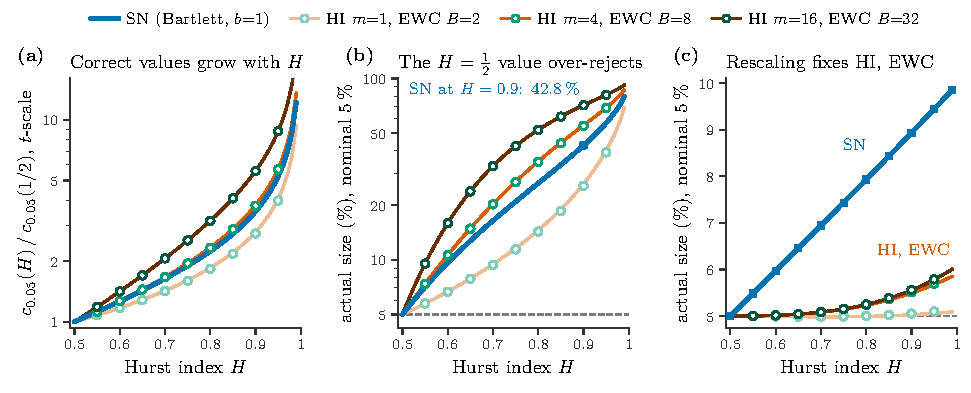
\includegraphics[width=\textwidth]{fig1_headline.pdf}
\caption{Critical values and limit size of the three test families. (a)~Two-sided $5\,\%$ critical values relative
to short-memory values ($t$ scale). (b)~Limit size of nominal $5\,\%$ tests using short-memory values.
(c)~As (b) after the rescaling of \cref{prop:rho} (narrower vertical range). Lines: HI, $m$ frequencies;
circles: EWC, $B=2m$; all values certified.}\label{fig:headline}
\end{figure}

\subsection{The Bartlett/self-normalised statistic}
\Cref{tab:sncv} gives the quantiles of $T_H$ for selected $H$; \cref{app:tables} gives all
\pthree{sn-n-H} values $H=0.50,0.51,\dots,0.99$ at the six levels $p\in\{0.80,0.90,0.95,0.975,0.98,0.99\}$, which cover
two-sided tests at $10$, $5$ and $1\,\%$ and one-sided tests with the signed statistics at $10$, $5$, $1.25$ and $1\,\%$.
A two-sided test at level $\alpha$ rejects when $T_n>q_{1-\alpha}$; a one-sided test at level $a$ with the signed
statistic $t$ of \citet{KV02} or \citet{MP12} ($T_H=2t^2$) rejects when $t>\sqrt{q_{1-2a}/2}$, and with the statistic of
\citet{KVB00} ($T_H=t^2$) when $t>\sqrt{q_{1-2a}}$.
Each value carries a certified enclosure: the largest relative half-width over the \pthree{sn-n-cells} cells is
\pthree{sn-max-relwidth}, attained at $H=\frac12$, and every printed value is the correctly rounded value of every number
in its enclosure. At $H=\frac12$
the values agree with the closed-form law of \citet{AP97} to \pthree{g0-min-digits} significant digits or more.

\begin{table}[tbp]\centering\small
\caption{Certified quantiles $q_p(H)$ of $T_H$; each entry is correctly rounded, so the number of digits varies.}\label{tab:sncv}
\begin{tabular}{@{}lrrrr@{}}\toprule
$H$ & $q_{0.80}$ & $q_{0.90}$ & $q_{0.95}$ & $q_{0.99}$\\\midrule
0.50 & 15.015 & 28.331 & 45.53 & 100.3\\
0.55 & 18.450 & 35.23 & 57.23 & 128.9\\
0.60 & 22.876 & 44.195 & 72.555 & 166.84\\
0.65 & 28.726 & 56.144 & 93.147 & 218.70\\
0.70 & 36.7212 & 72.6087 & 121.741 & 291.854\\
0.75 & 48.1606 & 96.3545 & 163.284 & 399.760\\
0.80 & 65.6455 & 132.920 & 227.701 & 569.48\\
0.85 & 95.2468 & 195.244 & 338.197 & 864.40\\
0.90 & 155.181 & 322.168 & 564.474 & 1475.24\\
0.95 & 336.540 & 707.966 & 1255.25 & 3356.71\\
0.99 & 1793.35 & 3814.26 & 6829.94 & 18613.1\\
\bottomrule\end{tabular}
%
\end{table}

The values grow quickly with memory: $q_{0.95}$ is multiplied by \pthree{sn-infl-0.80-0.950} between $H=\frac12$ and
$H=0.8$ and by \pthree{sn-infl-0.99-0.950} up to $H=0.99$. On the $t$ scale of \cref{fig:headline}a, where the
Bartlett/self-normalised value is shown as $\sqrt{q_{0.95}(H)/q_{0.95}(\frac12)}$, this is a factor
\pthree{sn-tinfl-0.99-0.950}.

\subsection{Fixed-smoothing statistics}
The fixed-$m$ and EWC limits are finite-dimensional, so their quantiles can be certified at every $0<H<1$
(\cref{prop:continuation}). \Cref{tab:fixedcv} gives two-sided $5\,\%$ values; \cref{app:tables} gives the
\pthree{fx-n-cells} certified values for $m=1,\dots,16$, $B\in\{1,2,3,4,6,8,12,16,24,32\}$, $\alpha\in\{0.10,0.05,0.01\}$
and $H=0.50,0.51,\dots,0.99$. At $H=\frac12$ every enclosure contains the Student-$t$ value with $2m$ or $B$ degrees of
freedom, which validates the computation against an independent closed form.

\begin{table}[tbp]\centering\small
\caption{Two-sided $5\,\%$ critical values of the fixed-$m$ statistic $\tau$ of \citet{HI17} and of the EWC statistic
of \citet{LLSW18} (certified). At $H=\frac12$ the values are $t_{2m,0.975}$ and $t_{B,0.975}$.}\label{tab:fixedcv}
\begin{tabular}{@{}lrrrrrrrrrr@{}}\toprule
 & \multicolumn{5}{c}{HI, $m$} & \multicolumn{5}{c}{EWC, $B$}\\\cmidrule(lr){2-6}\cmidrule(l){7-11}
$H$ & 1 & 2 & 4 & 8 & 16 & 2 & 4 & 8 & 16 & 32\\\midrule
0.50 & 4.3027 & 2.7764 & 2.3060 & 2.1199 & 2.0369 & 4.3027 & 2.7764 & 2.3060 & 2.1199 & 2.0369\\
0.60 & 5.0406 & 3.3665 & 2.9219 & 2.8287 & 2.8790 & 5.0366 & 3.3639 & 2.9203 & 2.8278 & 2.8785\\
0.70 & 6.1325 & 4.2418 & 3.8430 & 3.9070 & 4.1964 & 6.1039 & 4.2278 & 3.8350 & 3.9023 & 4.1937\\
0.80 & 7.9547 & 5.6995 & 5.3800 & 5.7228 & 6.4550 & 7.8712 & 5.6595 & 5.3569 & 5.7089 & 6.4466\\
0.90 & 11.978 & 8.8891 & 8.7220 & 9.6670 & 11.386 & 11.767 & 8.7863 & 8.6618 & 9.6299 & 11.363\\
0.95 & 17.517 & 13.228 & 13.221 & 14.933 & 17.933 & 17.139 & 13.042 & 13.111 & 14.864 & 17.889\\
0.99 & 40.278 & 30.842 & 31.269 & 35.829 & 43.650 & 39.276 & 30.343 & 30.970 & 35.640 & 43.529\\
\bottomrule\end{tabular}
%
\end{table}

The columns for HI with $m$ frequencies and EWC with $B=2m$ cosines are close at every $H$, although the two
self-normalisers use different coordinates (\cref{prop:coords}b); the same near-equality holds for power
(\cref{sec:power}).

\subsection{The price of the short-memory critical value}
\Cref{fig:headline}b shows the exact limit size of the nominal $5\,\%$ tests that keep the short-memory value. At $H=0.7$
the Bartlett/self-normalised test rejects a true null \pthree{naive-sn-0.70-0.05}\,\% of the time and at $H=0.9$
\pthree{naive-sn-0.90-0.05}\,\%. The fixed-smoothing tests are worse, and they are the worse the more components their
variance estimator has: at $H=0.9$ the size is \pthree{naive-hi1-0.90}\,\% for $m=1$ and \pthree{naive-hi16-0.90}\,\%
for $m=16$. The variance estimators that use more frequencies average periodogram ordinates further from the origin,
whose expectation is smaller under long memory, and they also have smaller critical values.

The same comparison can be made on data of a fixed length, where no limit argument is involved. \Cref{tab:matched} holds
the data model and the sample size fixed (fractional Gaussian noise, $n=64$ and $128$) and changes only the critical value
of the squared statistic $T_n$. With the Brownian value $45.526$ the exact size is
\pthree{mx-0.90-128}\,\% at $H=0.9$ and \pthree{mx-0.99-128}\,\% at $H=0.99$ for $n=128$; with the certified value
\pthree{mx-cv-0.99} for $H=0.99$ it is \pthree{mx-0.99-128-own}\,\%. Under long memory the finite-grid sizes differ from
the certified limit sizes by at most \pthree{mx-gap-64-long}\,pp at $n=64$ and \pthree{mx-gap-128-long}\,pp at $n=128$;
the largest gap, \pthree{mx-gap-64}\,pp, is the short-memory one at $H=\pthree{mx-gap-64-H}$ and $n=64$. For fractional
Gaussian noise the limit critical values therefore already apply at these sample sizes. The
entries are exact finite-dimensional laws, computed twice, by the series of \cref{prop:exactn} and by an independent
Imhof integral at $30$ digits, which agree to \pthree{mx-maxdiff-AB}\,pp; they also reproduce an independent
double-precision check to the printed digits (largest difference \pthree{mx-maxdiff-user}\,pp).

\begin{table}[tbp]\centering\small
\caption{Exact size (\%) under fractional Gaussian noise of the test that rejects when $T_n$ exceeds the stated value;
finite-$n$ columns are exact laws (\cref{prop:exactn}), the last column the certified limit.}\label{tab:matched}
\begin{tabular}{@{}llrrr@{}}\toprule
& & \multicolumn{2}{c}{exact, finite grid} & limit\\\cmidrule(lr){3-4}\cmidrule(l){5-5}
$H$ & critical value used & $n=64$ & $n=128$ & certified\\\midrule
0.50 & $H=\frac12$ value $45.526$ & 5.0167 & 5.0042 & 5.0000\\
0.90 & $H=\frac12$ value $45.526$ & 42.8085 & 42.8081 & 42.8080\\
0.99 & $H=\frac12$ value $45.526$ & 79.5227 & 79.5227 & 79.5227\\
0.99 & rounded certified value $6829.9$ & -- & 5.00008 & 5.0000\\
0.99 & certified value $6829.9404$ & -- & 5.00004 & 5.0000\\
\bottomrule\end{tabular}
%
\end{table}

\subsection{Why the critical values grow: collapse of the self-normaliser}\label{sec:collapse}
As $H\uparrow1$ the fractional Brownian path becomes linear, $\E|B_H(r)-rB_H(1)|^2\to0$ uniformly in $r$, so every
self-normaliser in \eqref{eq:limits} tends to zero while the numerator keeps unit variance. The rate is explicit.

\begin{proposition}[First moments of the self-normalisers]\label[proposition]{prop:rho}
Let $0<H<1$ and, for each procedure $P$, let $\rho_P(H)=\E D_P/\E_{1/2}D_P$. Then
\begin{gather*}\rho_{\SN}(H)=\frac{6}{(2H+1)(H+1)}-1,\qquad \rho_{\EWC,B}(H)=\frac1B\sum_{j=1}^BG_{jj},\\
\rho_{\HI,m}(H)=\frac1{2m}\sum_{j=1}^m\big(G_{2j,2j}+\Cov(\Sigma_{2j},\Sigma_{2j})\big),\end{gather*}
with the entries of \cref{prop:coords}. Each $\rho_P$ is real-analytic on $(0,1)$, equals $1$ at $H=\frac12$, and
$\rho_P(H)\to0$ as $H\uparrow1$; in particular $\rho_{\SN}(H)=\frac76(1-H)+O((1-H)^2)$.
\end{proposition}

The first moment alone does not determine how fast the critical values grow; the whole self-normaliser does, and it
collapses at rate $1-H$.

\begin{proposition}[Growth as $H\uparrow1$]\label[proposition]{prop:edge}
Let $\varphi(x)=x^2\log x$ ($\varphi(0)=0$) and
$k_1(r,s)=\varphi(|r-s|)-\varphi(r)-\varphi(s)+s\{\varphi(r)-\varphi(1-r)\}+r\{\varphi(s)-\varphi(1-s)\}$, which is
$-\partial_H\Cov(\Bt(r),\Bt(s))$ at $H=1$. As $H\uparrow1$, $(1-H)\,T_H\Rightarrow Z^2/\!\int_0^1G^2$, where $G$ is a
centred Gaussian process with covariance $k_1$, independent of $Z$, and $\int_0^1\E G(r)^2\dd r=\frac7{36}$. Hence
$(1-H)\,q_p(H)\to C_p$, the $p$-quantile of $Z^2/\!\int_0^1G^2$, for every $0<p<1$. The same holds for $\tau_{H,m}^2$
and $t_{H,B}^2$, for every $m\ge1$ and $B\ge1$, with the corresponding quadratic form in $G$; in particular
$\lim_{H\uparrow1}\rho_{\EWC,B}(H)/(1-H)\ge h_B/B$ and $\lim_{H\uparrow1}\rho_{\HI,m}(H)/(1-H)\ge h_m/(4m)$, where
$h_j=\sum_{i\le j}1/i$.
\end{proposition}

Numerically (a Nystr\"om discretisation of $k_1$ and Imhof's inversion; computed, not certified),
$C_{0.90}=\pthree{edge-C-0.900}$, $C_{0.95}=\pthree{edge-C-0.950}$ and $C_{0.99}=\pthree{edge-C-0.990}$, and the linear
extrapolation of the certified $(1-H)\,q_p(H)$ from $H=0.98$ and $0.99$ agrees with $C_p$ to within
\pthree{edge-extrap-maxrel}\,\% at all six levels. For the fixed-smoothing statistics the lower bounds of the proposition are attained with room to spare: at $H=0.999$,
$\rho_P(H)/(1-H)$ is at least \pthree{edge-rho-min} for the tabulated $m\le16$ and $B\in\{1,2,3,4,6,8,12,16,24,32\}$
(computed).

If the components of a fixed-smoothing self-normaliser were independent of $Z$ and equally scaled, as they are at
$H=\frac12$, then $\rho_P(H)^{-1/2}$ times the Student-$t$ value would be the exact critical value. Under long memory
neither condition holds, but the departure from them turns out to matter little: the rule
\begin{equation}\label{eq:rescaled}
\text{reject when }|\tau_{n,m}|>t_{2m,1-\alpha/2}\big/\sqrt{\rho_{\HI,m}(H)}\quad\text{or}\quad
|t_{n,B}|>t_{B,1-\alpha/2}\big/\sqrt{\rho_{\EWC,B}(H)}
\end{equation}
has exact limit size within \pthree{rs-maxerr-090-0.10}, \pthree{rs-maxerr-090-0.05} and \pthree{rs-maxerr-090-0.01}\,pp
of $10$, $5$ and $1\,\%$ for every $m\le16$, every $B\in\{1,2,3,4,6,8,12,16,24,32\}$ and $H=0.50,0.51,\dots,0.90$, and within
\pthree{rs-maxerr-099-0.05}\,pp at $5\,\%$ up to $H=0.99$ (\cref{fig:headline}c, \cref{tab:rescaled}). Only $\rho(H)$, a
finite sum of closed-form Gram entries, is needed. Memory corrections of the long-run variance estimator itself were
proposed by \citet{Rob05} and \citet{ADG09}; \eqref{eq:rescaled} instead corrects the critical value of an uncorrected
estimator, and its size error is known exactly. For the Bartlett/self-normalised statistic the corresponding rule
$T_n>q_{1-\alpha}(\frac12)/\rho_{\SN}(H)$ is not adequate: its $5\,\%$ size is \pthree{rs-sn-0.75-0.05}\,\% at $H=0.75$
and \pthree{rs-sn-0.95-0.05}\,\% at $H=0.95$. Its numerator and denominator are coupled through every even cosine
coordinate, and its denominator is dominated by the first few coordinates, whose relative weights change with $H$.

\begin{table}[tbp]\centering\small
\caption{Largest deviation (percentage points) of the exact limit size of the rescaled rule \eqref{eq:rescaled} from the
nominal level, over $m=1,\dots,16$ and $B\in\{1,2,3,4,6,8,12,16,24,32\}$ (certified enclosures of the size).}\label{tab:rescaled}
\begin{tabular}{@{}lcccccc@{}}\toprule
 & \multicolumn{3}{c}{HI, $m\le16$} & \multicolumn{3}{c}{EWC, tabulated $B$}\\
\cmidrule(lr){2-4}\cmidrule(l){5-7}
$H$ & $10\,\%$ & $5\,\%$ & $1\,\%$ & $10\,\%$ & $5\,\%$ & $1\,\%$\\\midrule
0.50--0.70 & 0.13 & 0.10 & 0.04 & 0.13 & 0.10 & 0.04\\
0.71--0.80 & 0.34 & 0.27 & 0.12 & 0.35 & 0.28 & 0.12\\
0.81--0.90 & 0.72 & 0.59 & 0.26 & 0.73 & 0.59 & 0.27\\
0.91--0.99 & 1.23 & 1.03 & 0.48 & 1.24 & 1.03 & 0.49\\
\bottomrule\end{tabular}
%
\end{table}

\subsection{A response surface}\label{sec:surface}
For use without tables we fit, for each level $p$, $\log q_p(H)=-\log(1-H)+\sum_{i=0}^{K}a_{p,i}(H-\frac12)^i$, which
builds in the rate $q_p(H)\sim C_p/(1-H)$ of \cref{prop:edge}. The coefficients are fitted to the certified values at even hundredths of $H$ only; the degree, $K=\pthree{rs-surface-K}$
for every level, is the smallest whose leave-one-out error on these points is below a tenth of their certification
error. The odd hundredths, used neither for the fit nor for the choice of $K$, are held out, and on them we report two
errors (\cref{tab:surface}). The held-out fit error, computed through the density, is at most
\pthree{rs-surface-fit-maxerr}\,pp in size against the tabulated values. The certified bound refers to the coefficients as printed (\pthree{rs-surface-digits} significant digits): the
surface value is evaluated exactly from them in ball arithmetic, and under the true law the resulting critical value has
size within \pthree{rs-surface-cert-maxerr}\,pp of nominal at every held-out $H$ and level. Where that value lies inside
the certified bracket, the bound follows from the enclosures of $F_H$ at the bracket ends by monotonicity; otherwise
($\pthree{rs-surface-cert-ndirect}$ of the $\pthree{rs-surface-cert-ncells}$ cases) $F_H$ is enclosed afresh at the two
floating-point neighbours of the value. The bound holds at the held-out points only: between them the surface is an
interpolation without a guarantee, and outside $\frac12\le H\le0.99$ it should not be used.
%
\section{Actual rejection rates at sample size \texorpdfstring{$n$}{n}}\label{sec:finite}

\subsection{Exact finite-sample laws}
Let $x=(x_1,\dots,x_n)^\top\sim N(\mu\mathbf 1,\Gamma_n)$ with a positive definite Toeplitz covariance $\Gamma_n$, and
let $y=x-\mu_0\mathbf 1$. Each of the three statistics is a ratio $(a^\top y)^2/y^\top My$ with $a=n^{-1/2}\mathbf 1$ and a
positive semi-definite $M$ with $M\mathbf 1=0$, so that the denominator does not depend on $\mu_0$: for $T_n$,
$M=n^{-2}D^\top D$ with $D$ the matrix that maps $x$ to the demeaned partial sums $(\hat S_k)$; for $\tau_{n,m}^2$ and $t_{n,B}^2$, $M$ has rank $2m$
or $B$ and is spanned by the Fourier or cosine vectors in \eqref{eq:tauHI}--\eqref{eq:tEWC}.

\begin{proposition}[Exact finite-sample laws]\label[proposition]{prop:exactn}
Under $H_0:\mu=\mu_0$, for $c>0$, the ratio $Q=(a^\top y)^2/(y^\top My)$ satisfies $P(Q\le c)=P\big(\sum_i\theta_i(c)\xi_i^2\le0\big)$, with $\xi_i$
independent standard normal and $\theta_i(c)$ the eigenvalues of $\Gamma_n^{1/2}(aa^\top-cM)\Gamma_n^{1/2}$, of which exactly
one is positive (because $Ma=0$ and $\Gamma_n$ is positive definite). (a)~For the fixed-smoothing statistics the law depends on $\Gamma_n$ only through the $(2m+1)$- or
$(B+1)$-dimensional covariance $C^\top\Gamma_nC$ of $a^\top x$ and the coordinates. (b)~For $T_n$, if
$\Gamma_n^{1/2}M\Gamma_n^{1/2}=U\operatorname{diag}(\vartheta)U^\top$ and $\beta=U^\top\Gamma_n^{1/2}a$, the characteristic
function of $\sum_i\theta_i(c)\xi_i^2$ is
$\prod_k(1+2\mathrm isc\vartheta_k)^{-1/2}\big(1-2\mathrm is\sum_k\beta_k^2/(1+2\mathrm isc\vartheta_k)\big)^{-1/2}$, so one
eigendecomposition serves every $c$.
\end{proposition}

Part~(b) is the matrix determinant lemma; implemented via a Cholesky-free Woodbury reduction of the demeaned
cumulative-sum covariance and a two-band adaptive Imhof quadrature (\cref{sec:methods}), it requires a one-off set-up of
\pthree{e5-T3-setup-s}\,s at $n=1000$ and then \pthree{e5-T3-query-s}\,s for each further cutoff, instead of
\pthree{e5-T3-imhof-s}\,s for a fresh eigendecomposition and inversion.

\begin{proposition}[Fractional Gaussian noise]\label[proposition]{prop:fgn}
If $u_t=B_H(t)-B_H(t-1)$, then for every $n$ the vector of statistics $(T_n,\tau_{n,m},t_{n,B})$ has the law of the same
statistics computed from the increments of the fractional Brownian path $B_H$ on the grid $\{t/n\}$. In particular
$T_n\overset d=Z^2\big/\big(n^{-1}\sum_{k=1}^n\Bt(k/n)^2\big)$, the rectangle-rule discretisation of $T_H$.
\end{proposition}

Under fractional Gaussian noise the finite-sample laws are therefore pure discretisations of the limit laws, with no
short-run dynamics, and they converge rapidly: at $n=64$ and $n=128$ under fGn, the exact sizes of $T_n$ at the Brownian
cutoff $45.526$ already lie within \pthree{mx-gap-64-long}\,pp and \pthree{mx-gap-128-long}\,pp of the certified limits
for $H\in\{0.90,0.99\}$ (\pthree{mx-0.90-128}\,\% at $H=0.90$ and \pthree{mx-0.99-128}\,\% at $H=0.99$ for $n=128$),
whereas substituting the certified $H=0.99$ cutoff \pthree{mx-cv-0.99} delivers exact size \pthree{mx-0.99-64-own}\,\% at
$n=64$ and \pthree{mx-0.99-128-own}\,\% at $n=128$ (verified independently against $30$-digit Imhof integration to
\pthree{mx-maxdiff-AB}\,pp). At $n=500$ and $H=0.7$ the exact size of the Bartlett/self-normalised test at its own limit
critical value differs from $5\,\%$ by \pthree{fgn-sn-0.70-500-dev}\,pp.

\subsection{Results}
\Cref{fig:finite} and \cref{tab:finite} report exact sizes for fractional Gaussian noise, ARFIMA$(0,d,0)$ and
ARFIMA$(1,d,0)$ with $\phi=\pm0.5$, $d=H-\frac12\in\{0,\allowbreak0.1,\allowbreak0.2,\allowbreak0.3,\allowbreak0.4\}$ and $n\in\{50,\allowbreak100,\allowbreak200,\allowbreak500,\allowbreak1000,\allowbreak2000\}$,
for the Bartlett/self-normalised test, the fixed-$m$ test with $m\in\{1,2,3,4,6,8,12,16\}$ and the EWC test with
$B\in\{4,8,12,16,24,32\}$, each test using its own limit critical value at the true $H$. Three conclusions hold for all of them.

\emph{Memory alone costs little.} Under fractional Gaussian noise and ARFIMA$(0,d,0)$ every procedure is within
\pthree{fn-maxdev-pure}\,pp of $5\,\%$ for every $n\ge50$ and every $H$ in the design.

\emph{Short-run dynamics cost a lot in small samples.} With $\phi=0.5$ at $n=50$, the fixed-$m$ test with $m=16$
rejects \pthree{fn-arfima1p-HI16-0.50-50}\,\% of the time at $H=0.5$ and \pthree{fn-arfima1p-HI16-0.90-50}\,\% at
$H=0.9$, the Bartlett/self-normalised test \pthree{fn-arfima1p-SN-0.50-50}\,\% and the test with $m=1$
\pthree{fn-arfima1p-HI1-0.50-50}\,\%; with $\phi=-0.5$ the tests are conservative, down to
\pthree{fn-arfima1m-HI16-0.50-50}\,\% for $m=16$. At $n=2000$ every procedure is within \pthree{fn-maxdev-2000}\,pp.

\emph{The more components, the larger the distortion.} The ordering by the number of components is the same at every
$H$ and $n$ in the design, and the EWC test with $B=2m$ behaves like the fixed-$m$ test with $m$ frequencies.

\begin{figure}[tbp]\centering
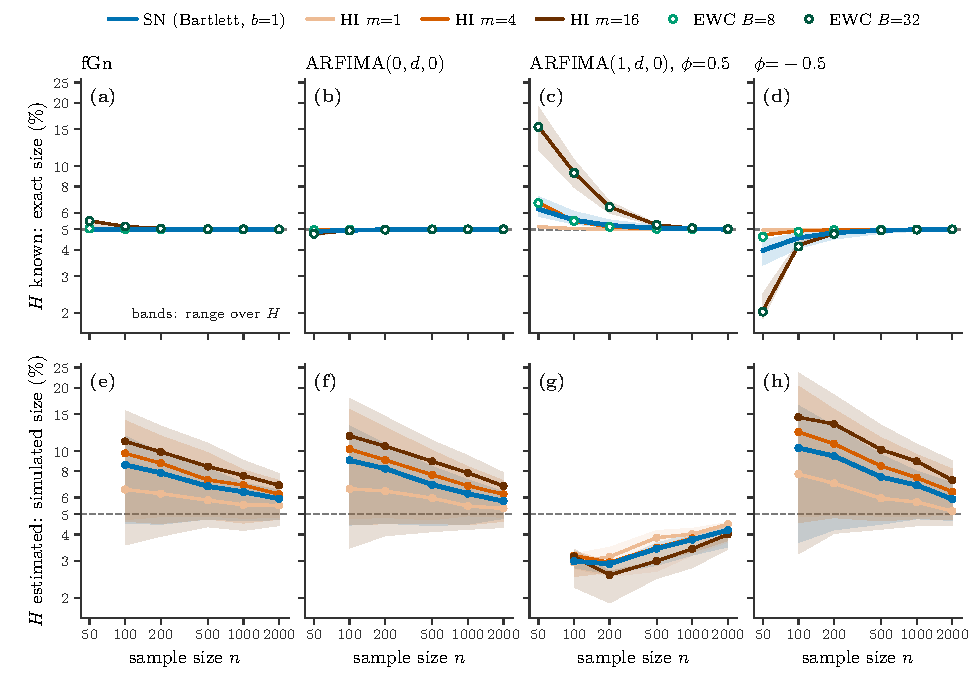
\includegraphics[width=\textwidth]{fig2_finite_n.pdf}
\caption{Finite-sample rejection rates at nominal 5\% with known memory (top) and estimated memory (bottom).}\label{fig:finite}
\end{figure}

\begin{table}[tbp]\centering\small
\caption{Exact rejection percentages at nominal 5\% using limit cutoffs at $H=0.7$.}\label{tab:finite}
\setlength{\tabcolsep}{4.5pt}\begin{tabular}{@{}llrrrrrr@{}}\toprule
model & test & $n=50$ & $n=100$ & $n=200$ & $n=500$ & $n=1000$ & $n=2000$\\\midrule
\multirow{6}{*}{fGn} & SN & 5.01 & 5.00 & 5.00 & 5.00 & 5.00 & 5.00\\
 & HI, $m=1$ & 5.00 & 5.00 & 5.00 & 5.00 & 5.00 & 5.00\\
 & HI, $m=4$ & 5.05 & 5.01 & 5.00 & 5.00 & 5.00 & 5.00\\
 & HI, $m=16$ & 5.49 & 5.16 & 5.05 & 5.01 & 5.00 & 5.00\\
 & EWC, $B=8$ & 5.05 & 5.01 & 5.00 & 5.00 & 5.00 & 5.00\\
 & EWC, $B=32$ & 5.48 & 5.16 & 5.05 & 5.01 & 5.00 & 5.00\\
\midrule
\multirow{6}{*}{ARFIMA$(0,d,0)$} & SN & 4.89 & 4.95 & 4.98 & 4.99 & 5.00 & 5.00\\
 & HI, $m=1$ & 5.00 & 5.00 & 5.00 & 5.00 & 5.00 & 5.00\\
 & HI, $m=4$ & 4.98 & 4.99 & 5.00 & 5.00 & 5.00 & 5.00\\
 & HI, $m=16$ & 4.77 & 4.94 & 4.98 & 5.00 & 5.00 & 5.00\\
 & EWC, $B=8$ & 4.97 & 4.99 & 5.00 & 5.00 & 5.00 & 5.00\\
 & EWC, $B=32$ & 4.77 & 4.94 & 4.98 & 5.00 & 5.00 & 5.00\\
\midrule
\multirow{6}{*}{ARFIMA$(1,d,0)$, $\phi=0.5$} & SN & 6.24 & 5.54 & 5.22 & 5.07 & 5.03 & 5.01\\
 & HI, $m=1$ & 5.15 & 5.04 & 5.01 & 5.00 & 5.00 & 5.00\\
 & HI, $m=4$ & 6.70 & 5.48 & 5.13 & 5.02 & 5.01 & 5.00\\
 & HI, $m=16$ & 15.44 & 9.33 & 6.40 & 5.25 & 5.07 & 5.02\\
 & EWC, $B=8$ & 6.66 & 5.49 & 5.14 & 5.03 & 5.01 & 5.00\\
 & EWC, $B=32$ & 15.38 & 9.29 & 6.39 & 5.25 & 5.07 & 5.02\\
\midrule
\multirow{6}{*}{ARFIMA$(1,d,0)$, $\phi=-0.5$} & SN & 3.97 & 4.55 & 4.82 & 4.95 & 4.98 & 4.99\\
 & HI, $m=1$ & 4.96 & 4.99 & 5.00 & 5.00 & 5.00 & 5.00\\
 & HI, $m=4$ & 4.70 & 4.91 & 4.97 & 4.99 & 5.00 & 5.00\\
 & HI, $m=16$ & 2.05 & 4.19 & 4.79 & 4.96 & 4.99 & 5.00\\
 & EWC, $B=8$ & 4.61 & 4.87 & 4.96 & 4.99 & 5.00 & 5.00\\
 & EWC, $B=32$ & 2.03 & 4.14 & 4.76 & 4.95 & 4.99 & 5.00\\

\bottomrule\end{tabular}
%
\end{table}

In \cref{fig:finite}, lines and markers follow $H=0.7$; the bands, drawn for SN and HI with $m=4$, span the grid
$H\in\{0.5,\dots,0.9\}$. Open circles mark EWC with $B=2m$. The lower panels use $40\,000$ replications per cell.

\paragraph{Validation} The exact computations were checked against independent Monte Carlo simulation with
\pthree{val-R} replications per cell, by the circulant-embedding sampler of \citet{DH87}: in
\pthree{val-n-inside} of \pthree{val-n-cells} cells the exact rate lies inside the $99\,\%$ Wilson interval, and the
standardised differences have mean \pthree{val-z-mean} and standard deviation \pthree{val-z-sd}, as they should if the
exact rates are correct (Supplementary Material Figure~S.1). A second, larger check comes from the estimated-$H$ study
below, whose \emph{oracle} rule uses the critical value at the true $H$: over its \pthree{or-n-cells} cells (four
models, $n=100,\dots,2000$, three levels) the exact rate lies inside the $99\,\%$ interval in \pthree{or-inside-pct}\,\%
of them, with standardised differences of mean \pthree{or-z-mean}, standard deviation \pthree{or-z-sd} and largest
absolute value \pthree{or-maxz}. The exact laws also reproduce the published rejection frequencies of
\citet[Table~2]{HI17} for the AR(1) design with $\phi=0.5$ at $T=64$ and $256$, with largest standardised difference
\pthree{hi17-t2-maxz} over the \pthree{hi17-t2-n} published cells.

\subsection{When \texorpdfstring{$H$}{H} is estimated}\label{sec:plugin}
In practice $H$ is unknown. We first estimate it by the local Whittle estimator \citep{Rob95} with bandwidth
$m_{\mathrm{LW}}=\lfloor n^{0.65}\rfloor$, as in \citet{HI17}, and plug the estimate into the limit critical value;
these rates are simulated. Reproducing Tables~3--5 of \citet{HI17}---Gaussian ARFIMA$(1,\delta,0)$ with
$(\delta,\phi)\in\{(0,0),(-0.3,0.5),(0.3,-0.5)\}$ and \pthree{hi17-R} replications (Supplementary Material Table~S.3)---confirms
their plug-in pattern: linearly interpolating their printed Table~1 differs from their published rates by
\pthree{hi17-meandiff}\,pp on average (\pthree{hi17-share-z2}\,\% of the \pthree{hi17-ncells} cells beyond two joint
standard errors, maximum \pthree{hi17-maxdiff}\,pp). The published description does not identify the source of the residual differences. Pairing those
plug-in rates with the \emph{exact} finite-$T$ oracle sizes from \cref{prop:exactn} (Supplementary Material Table~S.3)
yields the central decomposition: with the true $\delta$ the fixed-$m$ test stays close to nominal (exactly $5.00\,\%$
under white noise), whereas with estimated $\delta$ the size reaches \pthree{hi17-T5-64-16-plugin}\,\% at $T=64$ in
their Table~5. On this grid the contrast measures the effect of estimating $H$ while holding the design and statistic fixed.

The same decomposition holds across our full design grid (\cref{fig:finite}, bottom row, and \cref{tab:plugin}), with
\pthree{pl-R} replications per cell and $\hat H$ clipped to $[\frac12,0.99]$ for every test so that all procedures
assume long memory a priori in the same way. Under fractional Gaussian noise and ARFIMA$(0,d,0)$ with $H\ge0.6$ the
feasible tests reject between \pthree{pl-pure-min-100} and \pthree{pl-pure-max-100}\,\% at $n=100$ and between
\pthree{pl-pure-min-2000} and \pthree{pl-pure-max-2000}\,\% at $n=2000$ (over $H\in\{0.6,0.7,0.8,0.9\}$), against at
most \pthree{fn-maxdev-pure}\,pp of distortion when $H$ is known. At $H=0.9$ and $n=100$ under fractional Gaussian noise
the Bartlett/self-normalised test rejects \pthree{pl-fgn-SN-0.9-100}\,\%, the fixed-$m$ test with $m=4$
\pthree{pl-fgn-HI4-0.9-100}\,\% and with $m=16$ \pthree{pl-fgn-HI16-0.9-100}\,\%. With estimated $H$ the distortion
grows with the number of components: in the \pthree{pl-n-pure-cells} pure-memory cells with $H\ge0.6$, HI with $m=1$
is less distorted than SN in \pthree{pl-share-hi1-le-sn}\,\% of cells and EWC with $B=4$ in \pthree{pl-share-ewc4-le-sn}\,\%,
whereas SN is less distorted than HI with $m=4$ and $16$ in \pthree{pl-share-sn-le-hi4}\,\% and than EWC with $B=8$ and $32$
in \pthree{pl-share-sn-le-ewc8}\,\%. The power ranking of \cref{sec:power} therefore comes with the opposite ranking in
feasible size. Positive short-run correlation biases $\hat H$ upwards and makes every feasible test conservative (sizes
between \pthree{pl-ar1p-min} and \pthree{pl-ar1p-max}\,\%); negative correlation biases $\hat H$ downwards, pushing
rejection rates up to \pthree{pl-ar1m-max-100}\,\% at $n=100$. Clipping matters only near $H=\frac12$: at $H=0.5$,
$n=100$, HI with $m=4$ rejects \pthree{pl-HI4-H05-trunc}\,\% with clipped $\hat H$ versus \pthree{pl-HI4-H05-untrunc}\,\%
unclipped.

\paragraph{Bandwidth sensitivity} Across local Whittle bandwidths $\lfloor n^{0.5}\rfloor$, $\lfloor n^{0.65}\rfloor$
and $\lfloor n^{0.8}\rfloor$ (common random numbers; full table in Supplementary Material Table~S.4), feasible sizes
under pure long memory ($H\in\{0.7,0.9\}$) span \pthree{bw-50-min-100}--\pthree{bw-50-max-100}\,\%,
\pthree{bw-65-min-100}--\pthree{bw-65-max-100}\,\% and \pthree{bw-80-min-100}--\pthree{bw-80-max-100}\,\% at $n=100$,
and \pthree{bw-50-min-2000}--\pthree{bw-50-max-2000}\,\%, \pthree{bw-65-min-2000}--\pthree{bw-65-max-2000}\,\% and
\pthree{bw-80-min-2000}--\pthree{bw-80-max-2000}\,\% at $n=2000$. Widening the bandwidth to $n^{0.8}$ lowers estimator
variance enough to keep fGn within \pthree{bw-80-fgn-maxdev-500}\,pp of nominal from $n=500$, but leaves ARFIMA$(0,d,0)$
distorted up to \pthree{bw-80-arfima0-max-500}\,\% and amplifies short-run bias \citep{Rob95}.

\begin{table}[tbp]\centering\small
\caption{Simulated rejection percentages at nominal 5\% using local Whittle estimates of memory.}\label{tab:plugin}
\begin{tabular}{@{}llrrrrrr@{}}\toprule
& & \multicolumn{3}{c}{$H=0.7$} & \multicolumn{3}{c}{$H=0.9$}\\\cmidrule(lr){3-5}\cmidrule(l){6-8}
model & test & $n=100$ & $500$ & $2000$ & $n=100$ & $500$ & $2000$\\\midrule
fGn & SN & 8.6 & 6.8 & 5.9 & 11.8 & 8.3 & 6.5\\
 & HI, $m=4$ & 9.7 & 7.3 & 6.2 & 14.0 & 9.8 & 7.2\\
 & HI, $m=16$ & 11.1 & 8.4 & 6.9 & 15.6 & 10.9 & 7.8\\
 & EWC, $B=8$ & 9.6 & 7.3 & 6.2 & 13.8 & 9.8 & 7.3\\
 & EWC, $B=32$ & 11.1 & 8.4 & 6.8 & 15.6 & 10.9 & 7.8\\
\addlinespace
ARFIMA$(0,d,0)$ & SN & 9.0 & 6.9 & 5.8 & 13.2 & 8.4 & 6.4\\
 & HI, $m=4$ & 10.2 & 7.7 & 6.2 & 15.8 & 10.1 & 7.2\\
 & HI, $m=16$ & 11.8 & 8.9 & 6.8 & 17.8 & 11.2 & 7.9\\
 & EWC, $B=8$ & 10.1 & 7.7 & 6.2 & 15.6 & 10.0 & 7.2\\
 & EWC, $B=32$ & 11.8 & 9.0 & 6.8 & 17.8 & 11.2 & 7.9\\
\addlinespace
ARFIMA$(1,d,0)$, $\phi=0.5$ & SN & 3.0 & 3.4 & 4.2 & 3.1 & 2.9 & 3.5\\
 & HI, $m=4$ & 3.2 & 3.5 & 4.1 & 3.4 & 3.0 & 3.7\\
 & HI, $m=16$ & 3.1 & 3.0 & 4.0 & 3.4 & 2.9 & 3.7\\
 & EWC, $B=8$ & 3.1 & 3.4 & 4.2 & 3.2 & 3.0 & 3.8\\
 & EWC, $B=32$ & 3.1 & 3.0 & 4.0 & 3.4 & 2.9 & 3.7\\
\addlinespace
ARFIMA$(1,d,0)$, $\phi=-0.5$ & SN & 10.3 & 7.5 & 5.9 & 16.4 & 9.6 & 7.0\\
 & HI, $m=4$ & 12.3 & 8.5 & 6.4 & 20.4 & 11.6 & 8.2\\
 & HI, $m=16$ & 14.5 & 10.1 & 7.3 & 23.5 & 13.3 & 9.0\\
 & EWC, $B=8$ & 12.2 & 8.4 & 6.5 & 20.2 & 11.5 & 8.1\\
 & EWC, $B=32$ & 14.3 & 10.1 & 7.3 & 23.5 & 13.3 & 9.0\\
\bottomrule\end{tabular}
%
\end{table}

\subsection{Competitor baselines and practical remedies under unknown \texorpdfstring{$H$}{H}}\label{sec:competitors}
We compare \CosCert{} plug-in rules, all with $\hat H$ truncated to $[\frac12,0.99]$ as in \cref{sec:plugin}, with four
feasible alternatives in \cref{tab:competitors} ($20\,000$ replications per design,
$n\in\{100,500\}$, $H\in\{0.5,0.7,0.9\}$, all four data models, measuring both null size and finite-sample local power
at $\mu_n=2.8\sqrt{\Var(\bar x_n)}$, where the Gaussian known-variance $z$-test has approximately $80\,\%$ power in every
design):
(i)~\emph{Exact Local Whittle (ELW) plug-in}---replacing Robinson's local Whittle with the demeaned exact local Whittle
estimator $\hat H_{\mathrm{ELW}}$ of \citet{SP05} and \citet{Shi10};
(ii)~\emph{Upper-confidence-bound plug-in}---evaluating \CosCert{} at the one-sided $90\,\%$ upper confidence bound
$\hat H_{\mathrm{up}}=\min\big(0.99,\,\hat H_{\mathrm{LW}}+z_{0.90}/(2\sqrt{m_{\mathrm{LW}}})\big)$ to guard directly
against downward estimation errors in $\hat H$;
(iii)~\emph{Memory- and autocorrelation-consistent (ADG--MAC) Studentisation} \citep{ADG09}---forming
$t_{\mathrm{MAC}}=n^{1/2-\hat d}\bar x/\hat V_{\mathrm{MAC}}^{1/2}$ with
$\hat V_{\mathrm{MAC}}=(2\pi\hat G)\,\Gamma(1-2\hat d)/\{(2\hat d+1)\Gamma(1+\hat d)\Gamma(1-\hat d)\}$ and
comparing $|t_{\mathrm{MAC}}|$ against $z_{0.975}=1.96$; and
(iv)~\emph{Rate-free self-normalised subsampling} \citep{PRW99,Sha10}---comparing $T_n$ against the empirical
distribution of overlapping centred sub-blocks $T_b^{(i)}$ of length $b=\operatorname{round}(n^{0.6})$ without
estimating $H$ at all.

\begin{table}[tbp]\centering\small
\caption{Simulated size and local power of feasible tests, in percent, at nominal 5\%.}\label{tab:competitors}
\footnotesize\setlength{\tabcolsep}{2.6pt}\begin{tabular}{@{}lcccccc@{}}\toprule
 & \multicolumn{2}{c}{fGn ($H=0.7$)} & \multicolumn{2}{c}{fGn ($H=0.9$)} & \multicolumn{1}{c}{$\phi{=}0.5$, $H{=}0.7$} & \multicolumn{1}{c}{$\phi{=}-0.5$, $H{=}0.7$}\\
\cmidrule(lr){2-3}\cmidrule(lr){4-5}\cmidrule(lr){6-6}\cmidrule(l){7-7}
procedure (size / power) & $n=100$ & $500$ & $n=100$ & $500$ & $n=500$ & $n=500$\\\midrule
SN (\CosCert{} LW) & 8.6 / 50.3 & 6.8 / 52.2 & 11.7 / 43.1 & 8.0 / 44.1 & 3.3 / 35.8 & 7.4 / 55.4\\
SN (\CosCert{} Upper-CI) & 4.5 / 31.2 & 3.8 / 37.9 & 4.9 / 20.1 & 3.3 / 21.7 & 1.5 / 20.8 & 4.4 / 41.6\\
HI $m{=}4$ (\CosCert{} LW) & 9.7 / 58.3 & 7.5 / 62.9 & 14.0 / 49.5 & 9.5 / 53.2 & 3.3 / 41.4 & 8.5 / 66.3\\
HI $m{=}4$ (\CosCert{} ELW) & 8.5 / 53.9 & 7.1 / 61.7 & 11.6 / 43.5 & 8.9 / 51.7 & 3.0 / 39.8 & 8.1 / 65.5\\
HI $m{=}4$ (\CosCert{} Upper-CI) & 4.6 / 34.5 & 3.8 / 44.2 & 5.5 / 22.0 & 3.6 / 25.1 & 1.2 / 22.4 & 4.5 / 48.7\\
EWC $B{=}8$ (\CosCert{} LW) & 9.6 / 58.3 & 7.5 / 62.6 & 13.9 / 49.5 & 9.4 / 53.2 & 3.3 / 41.5 & 8.5 / 66.3\\
ADG--MAC ($N(0,1)$) & 13.5 / 64.9 & 9.4 / 70.3 & 16.4 / 53.0 & 11.2 / 58.5 & 3.0 / 42.3 & 11.0 / 75.3\\
Subsampling SN (rate-free) & 15.8 / 67.6 & 11.3 / 62.4 & 27.8 / 79.0 & 20.5 / 72.9 & 9.5 / 57.2 & 12.6 / 66.1\\
\bottomrule\end{tabular}
%
\end{table}

\Cref{tab:competitors} reports six of the \pthree{comp-n-designs} designs. For the fixed-$m$ test with $m=4$, replacing
local Whittle (LW) by demeaned exact local Whittle (ELW) moves the simulated size closer to $5\,\%$ in exactly the
\pthree{comp-elw-closer} designs with $H>\frac12$ and no positive short-run correlation. In the other
\pthree{comp-elw-further} designs the LW rule already rejects too rarely---under positive AR, and at $H=\frac12$, where
truncation holds it at \pthree{comp-hi4-lw-h05-min}--\pthree{comp-hi4-lw-h05-max}\,\%---and ELW lowers rejection further.
Under fractional Gaussian noise at $H=0.9$ and $n=100$, ELW reduces size from \pthree{comp-hi4-lw-fgn-09-100}\,\% to
\pthree{comp-hi4-elw-fgn-09-100}\,\%.

For the four-frequency test, the upper-confidence-bound rule reduces rejection. At $n=500$ its simulated size is at most
\pthree{comp-hi4-up-n500-max}\,\% in all \pthree{comp-n500-designs} designs, against up to \pthree{comp-hi4-lw-n500-max}\,\%
for the LW rule and \pthree{comp-hi4-elw-n500-max}\,\% for the ELW rule. At $n=100$ it cuts the worst case, the
negative-AR design at $H=0.9$, from \pthree{comp-hi4-lw-ar1m-09-100}\,\% to \pthree{comp-hi4-up-ar1m-09-100}\,\%. The price
is power: under fractional Gaussian noise at $H=0.7$ and $n=500$, power falls from \pthree{comp-hi4-lw-fgn-07-500-pw}\,\%
to \pthree{comp-hi4-up-fgn-07-500-pw}\,\%.

At $H=0.9$ under fractional Gaussian noise, subsampling rejected a true null in \pthree{comp-sub-fgn-09-100}\,\% of
samples at $n=100$ and \pthree{comp-sub-fgn-09-500}\,\% at $n=500$. MAC and subsampling also had higher rejection
under the alternative in several designs. These are raw powers at a common nominal level, so differences in actual
size contribute to the comparison.
%
\section{Power and the choice of test}\label{sec:power}

Size is only half of the choice. Consider local alternatives $\mu-\mu_0=c\,\sigma n^{H-1}$, under which
$\sqrt n(\bar x-\mu_0)/(\sigma n^{H-1/2})\to Z+c$ while every self-normaliser keeps its null limit. In this section $c$ denotes this drift; critical values are written $q$.

\begin{proposition}[Local power of a finite-dimensional statistic]\label[proposition]{prop:power}
Let the self-normaliser be a finite quadratic form $D_P=\sum_{k=1}^Kw_kV_k^2$ in Gaussian components, let
$V=(Z,V_1,\dots,V_K)\sim N(0,\Sigma)$ with $\Sigma$ positive definite, and let
$A=\operatorname{diag}(1,-q\,w_1,\dots,-q\,w_K)$, where $q$ is the critical value of the squared statistic. Let
$\Sigma=LL^\top$, $L^\top AL=P\Theta P^\top$ and $\psi=\Theta^{-1}P^\top L^\top Ae_1c$. Then the limit power at $c$ is the
noncentral weighted chi-square probability
\[P\Big(\sum_i\Theta_{ii}(\xi_i+\psi_i)^2>0\Big),\qquad \xi_i\ \text{independent standard normal}.\]
\end{proposition}

We evaluate it by the noncentral form of Imhof's inversion \citep{Imh61}. For the fixed-smoothing statistics $K$ is
finite and the power is exact up to quadrature error. The self-normaliser of $T_H$ has infinitely many components; we
truncate it at $J=512$ cosine coordinates (\cref{prop:coords}) and replace the remainder by its mean, so its power is
computed rather than certified. Over every $H$ and $c$ of our grid it changes by at most \pthree{pw-jl-256-512} from
$J=256$ to $J=512$ and by at most \pthree{pw-jl-512-1024} from $J=512$ to $J=1024$. At $c=0$ the computed power equals
the nominal level to within \pthree{pw-c0-maxdev}, and at $H=\frac12$ the fixed-smoothing power equals the noncentral
Student-$t$ power to within \pthree{pw-nct-maxdev} in all \pthree{pw-nct-ncells} cells.

\begin{figure}[tbp]\centering
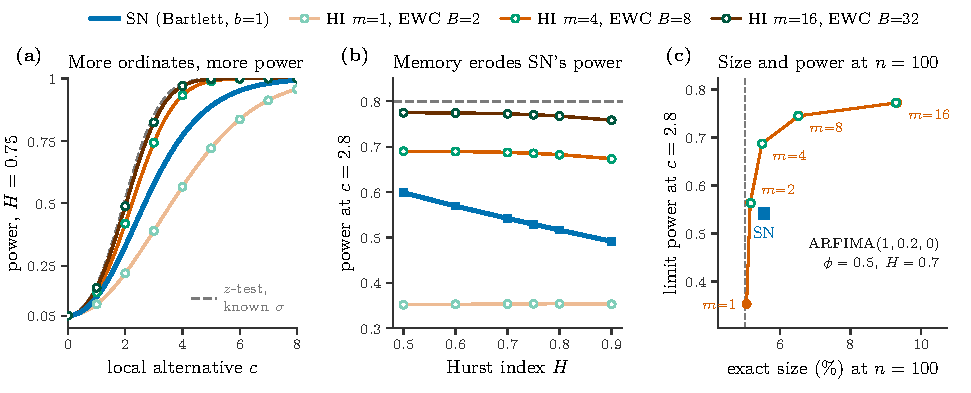
\includegraphics[width=\textwidth]{fig3_power.pdf}
\caption{Limit power and the size--power trade-off. (a)~Power at $H=0.75$ against the local alternative $c$; dashed:
infeasible $z$-test. (b)~Power at $c=2.8$ against $H$. (c)~Power at $c=2.8$ against exact size at $n=100$ under
ARFIMA$(1,0.2,0)$, $\phi=0.5$; open circles: EWC, $B=2m$; square: Bartlett/self-normalised test.}\label{fig:power}
\end{figure}

\Cref{fig:power} shows three regularities.
\emph{(i) Power grows with the number of components.} At $H=0.75$ and $c=2.8$ the power is \pthree{pw-HI1-0.75} for
$m=1$, \pthree{pw-HI4-0.75} for $m=4$ and \pthree{pw-HI16-0.75} for $m=16$, against \pthree{pw-z} for the infeasible
$z$-test that knows the scale $\sigma$ of the partial sums. The fixed-$m$ test with $m$ frequencies and the EWC test with $B=2m$ cosines have the same power to within
\pthree{pw-hi-ewc-maxdiff} at every $H$ and $c$ in our grid.
\emph{(ii) Memory erodes the power of the Bartlett/self-normalised test, but hardly that of the fixed-smoothing tests.}
From $H=\frac12$ to $H=0.9$ the power at $c=2.8$ of the former falls from \pthree{pw-SN-0.50} to \pthree{pw-SN-0.90}; that
of the fixed-$m$ test with $m=16$ changes from \pthree{pw-HI16-0.50} to \pthree{pw-HI16-0.90}.
\emph{(iii) Under short-run dynamics, power costs finite-sample size.} Each additional component raises power and,
in the design of \cref{fig:power}c, the finite-sample distortion; this is the size--power trade-off of \citet{LLS21} in the
long-memory setting.

\paragraph{Which test} With the critical value of the true $H$, the Bartlett/self-normalised test is dominated, in the
sense of a larger exact finite-sample size distortion together with a lower limit power against local alternatives
(power at finite $n$ is not computed here): at
$n=100$, $H=0.7$ and $\phi=0.5$ the fixed-$m$ test with $m=4$ has size \pthree{fn-arfima1p-HI4-0.70-100}\,\% and power
\pthree{pw-HI4-0.70}, against \pthree{fn-arfima1p-SN-0.70-100}\,\% and \pthree{pw-SN-0.70} for the former, and the
fixed-$m$ test with $m=4$ has both the smaller finite-sample size distortion and the higher limit power in
\pthree{dominance-share} of the
\pthree{dominance-ncells} $(H,n,\text{model})$ cells of our design. In limit power alone, the fixed-$m$ test with $m=4$ (EWC, $B=8$) exceeds the
Bartlett/self-normalised test in all \pthree{pw-vsSN-ncells} $(H,c)$ cells of the grid with $c>0$, with $m=2$ ($B=4$)
in \pthree{pw-vsSN-HI2-npos} (\pthree{pw-vsSN-EWC4-npos}), and with $m=1$ ($B=2$) in none. Fixed-smoothing tests with $m\le4$ frequencies, or
EWC tests with $B\in\{4,8\}$, are within \pthree{fn-maxdev-small-100}\,pp of $5\,\%$ for $n\ge100$ in every design and keep
most of the attainable power; tests with many components are preferable only when $n$ is large or short-run dynamics are
known to be weak.
%
\section{Empirical applications}\label{sec:empirical}

We compare short-memory and plug-in critical values on three contiguous series (\cref{fig:empirical,tab:empirical}).
The examples span local Whittle estimates of $H$ from \pthree{emp-aus-hlw} to \pthree{emp-nile-hlw}.
\begin{enumerate}
\item \emph{New South Wales electricity demand.} We aggregate half-hourly load from the Monash archive \citep{God21,MonashNSW}
to daily energy $D_t$ and test whether mean year-over-year growth $100\log(D_t/D_{t-365})$ is zero.
The $1095$ observations from March 2012 to February 2015 average \pthree{emp-aus-xbar}\,\%.
\item \emph{London air quality.} At Greenwich--Westhorne Avenue (GR9), we take the logarithm of each daily mean
$\mathrm{PM}_{2.5}$ concentration, in $\mu\mathrm{g}/\mathrm{m}^3$. From 1 January 2017 to 30 March 2018,
all 454 days have observations. The hourly archive \citep{MonashGR9} has 76 missing readings across 32 of those days;
each daily mean uses the available hours. We compare the geometric mean with two illustrative reference
concentrations, 10 and 15. The sample geometric mean is \pthree{emp-lon-geom}, and the arithmetic mean is
\pthree{emp-lon-arith}\,$\mu\mathrm{g}/\mathrm{m}^3$.
\item \emph{Nile annual minima.} The Roda Gauge series comprises 663 annual minimum water levels from AD 622 to 1284
\citep{Tou25,Hur51,Ber94}. We use 1100\,cm as a reference and obtain a sample mean of \pthree{emp-nile-xbar}\,cm.
\end{enumerate}

In \cref{fig:empirical}, coloured end marks identify plug-in intervals that change the decision relative to the grey interval.
For the plug-in tests, the archive interpolates the critical value at $\hat H_{\mathrm{LW}}$. It encloses the
limiting tail probability with $H$ fixed at that estimate rounded to four decimal places. These bounds quantify
numerical error. The sampling variability of $\hat H$ affects the rejection rates of feasible tests
(\cref{sec:competitors}). The last column of \cref{tab:empirical} gives the rejection rate of the short-memory cutoff
under a fitted Gaussian ARFIMA$(0,\hat d_{\mathrm{LW}},0)$ model. Daggers identify changed decisions at $5\,\%$;
the interval ratio is plug-in width divided by short-memory width. MAC and subsampling use their own reference laws.

\begin{figure}[tbp]\centering
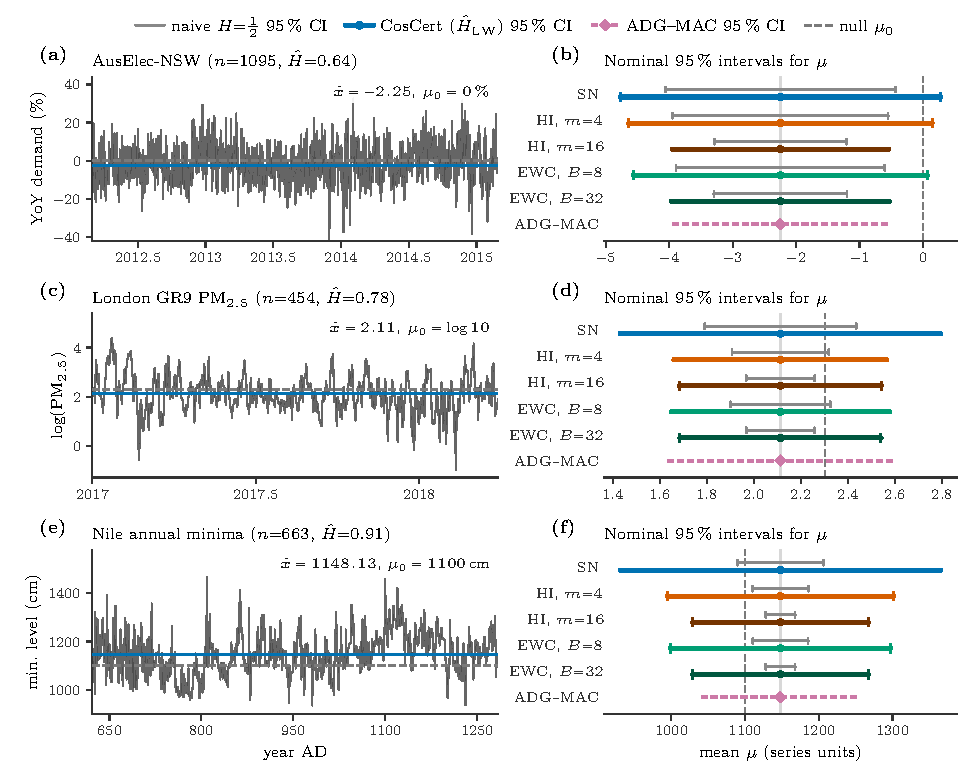
\includegraphics[width=\textwidth]{fig7_empirical.pdf}
\caption{Observed series and nominal 95\% intervals for mean electricity growth, log particulate concentration and Nile minima.}\label{fig:empirical}
\end{figure}

\begin{table}[tbp]\centering\small
\caption{Short-memory and plug-in tests of three series means. Daggers mark decisions that change at 5\%.}\label{tab:empirical}
\footnotesize\setlength{\tabcolsep}{2.2pt}\begin{tabular}{@{}llrrrrrrr@{}}\toprule
series & test & stat & \multicolumn{2}{c}{$5\,\%$ cutoff} & \multicolumn{2}{c}{$p$-value} & CI & naive\\
\cmidrule(lr){4-5}\cmidrule(lr){6-7}
($\hat H_{\mathrm{LW}}/\hat H_{\mathrm{ELW}}$, $n$, $\mu_0$) & & & naive & \CosCert{} & naive & \CosCert{} & ratio & size (\%)\\\midrule
AusElec-NSW & SN$^\dagger$ & 70.19 & 45.53 & 88.83 & 0.022 & 0.071 & 1.40$\times$ & 12.1\\
$\hat H{=}0.641/0.645$ & HI, $m{=}4$$^\dagger$ & $-3.05$ & 2.31 & 3.25 & 0.016 & 0.062 & 1.41$\times$ & 14.0\\
$n{=}1095$, $\mu_0{=}0\,\%$ & HI, $m{=}16$ & $-4.40$ & 2.04 & 3.34 & $<0.001$ & 0.012 & 1.64$\times$ & 22.3\\
 & EWC, $B{=}8$$^\dagger$ & $-3.15$ & 2.31 & 3.25 & 0.014 & 0.056 & 1.41$\times$ & 14.0\\
 & EWC, $B{=}32$ & $-4.37$ & 2.04 & 3.34 & $<0.001$ & 0.012 & 1.64$\times$ & 22.3\\
 & ADG--MAC / Sub.\ SN & $-2.58$ / -- & \multicolumn{2}{c}{1.96 / --} & \multicolumn{2}{c}{0.010 / 0.135} & -- & --\\
\midrule
London GR9 & SN & 15.73 & 45.53 & 204.04 & 0.192 & 0.454 & 2.12$\times$ & 24.6\\
$\hat H{=}0.784/0.791$ & HI, $m{=}4$ & $-2.12$ & 2.31 & 5.07 & 0.067 & 0.361 & 2.20$\times$ & 32.3\\
$n{=}454$, $\mu_0{=}\log 10$ & HI, $m{=}16$$^\dagger$ & $-2.65$ & 2.04 & 6.00 & 0.012 & 0.373 & 2.95$\times$ & 49.2\\
 & EWC, $B{=}8$ & $-2.06$ & 2.31 & 5.05 & 0.074 & 0.373 & 2.19$\times$ & 32.1\\
 & EWC, $B{=}32$$^\dagger$ & $-2.65$ & 2.04 & 5.99 & 0.012 & 0.371 & 2.94$\times$ & 49.1\\
 & ADG--MAC / Sub.\ SN & $-0.77$ / -- & \multicolumn{2}{c}{1.96 / --} & \multicolumn{2}{c}{0.440 / 0.276} & -- & --\\
\midrule
Nile minima & SN & 30.98 & 45.53 & 632.75 & 0.089 & 0.522 & 3.73$\times$ & 44.9\\
$\hat H{=}0.909/0.908$ & HI, $m{=}4$$^\dagger$ & 2.91 & 2.31 & 9.26 & 0.020 & 0.482 & 4.02$\times$ & 57.5\\
$n{=}663$, $\mu_0{=}1100\,\mathrm{cm}$ & HI, $m{=}16$$^\dagger$ & 4.92 & 2.04 & 12.18 & $<0.001$ & 0.409 & 5.98$\times$ & 73.0\\
 & EWC, $B{=}8$$^\dagger$ & 2.96 & 2.31 & 9.19 & 0.018 & 0.471 & 3.99$\times$ & 57.2\\
 & EWC, $B{=}32$$^\dagger$ & 4.92 & 2.04 & 12.15 & $<0.001$ & 0.408 & 5.97$\times$ & 73.0\\
 & ADG--MAC / Sub.\ SN & 0.88 / -- & \multicolumn{2}{c}{1.96 / --} & \multicolumn{2}{c}{0.381 / 0.272} & -- & --\\
\midrule
London GR9 & SN$^\dagger$ & 155.15 & 45.53 & 204.04 & 0.003 & 0.073 & 2.12$\times$ & 24.6\\
$\hat H{=}0.784/0.791$ & HI, $m{=}4$ & $-6.66$ & 2.31 & 5.07 & $<0.001$ & 0.016 & 2.20$\times$ & 32.3\\
$n{=}454$, $\mu_0{=}\log 15$ & EWC, $B{=}8$ & $-6.46$ & 2.31 & 5.05 & $<0.001$ & 0.019 & 2.19$\times$ & 32.1\\
 & ADG--MAC / Sub.\ SN & $-2.42$ / -- & \multicolumn{2}{c}{1.96 / --} & \multicolumn{2}{c}{0.015 / 0.005} & -- & --\\
\bottomrule\end{tabular}
%
\end{table}

In New South Wales all five tests reject zero mean growth with the short-memory cutoffs. With plug-in calibration,
three change decision: SN ($p=\pthree{emp-aus-SN-pcc}$), HI with $m=4$ ($p=\pthree{emp-aus-HI4-pcc}$)
and EWC with $B=8$ ($p=\pthree{emp-aus-EWC8-pcc}$). HI with $m=16$ and EWC with $B=32$ still reject.
The choice of smoothing therefore matters even when the memory estimate is held fixed.

For London, HI with $m=16$ changes from $p=\pthree{emp-lon-HI16-pnv}$ to $p=\pthree{emp-lon-HI16-pcc}$
at the reference concentration of 10. At the reference of 15, SN gives $p=\pthree{emp-lon15-SN-pcc}$,
while HI with $m=4$ and EWC with $B=8$ give $p=\pthree{emp-lon15-HI4-pcc}$ and
$p=\pthree{emp-lon15-EWC8-pcc}$. These comparisons concern the mean of log concentration over the observed period.

For the Nile, all four fixed-smoothing tests change from rejection to non-rejection. The widest relative change
occurs for HI with $m=16$: its interval expands by a factor of \pthree{emp-nile-HI16-ratio}, and its plug-in
$p$-value is \pthree{emp-nile-HI16-pcc}. LW and demeaned ELW give the same decisions in all three series.

\FloatBarrier
%
\section{An audit of published critical values in size units}\label{sec:audit}

A published critical value $\hat c$ for nominal level $\alpha$ is judged by the size it actually delivers,
$P(\text{statistic}>\hat c)$ under the law it is meant for, not by its relative error: near the tail of a heavy-tailed
law a $1\,\%$ error in $\hat c$ can be negligible or important depending on the density there. For every value in the
ledger (\cref{app:audit}) we record the source, page and table; the statistic and its normalisation (\cref{tab:norm});
the tail; the simulation design and number of replications $N$; and the version of the document that was read. We
then compute the true size, certified where the law is certified, and compare its deviation from $\alpha$ with the Monte
Carlo standard error of the source's own design, $\sqrt{\alpha(1-\alpha)/N}$. The verdict rules were fixed before the
computation: a value is \emph{accurate within Monte Carlo error} if its size deviation is within three standard errors.
The protocol allowed the word \emph{inaccurate} for deviations that the stated design does not explain or that exceed
$0.1$\,pp at the $5\,\%$ level; we use it only in the first, stricter sense, for values more than three standard errors
from nominal under the law they are meant for (class~E), and describe the others by their class. Each value receives
one of five classes, assigned in this order. A value more than three standard errors from nominal in the limit is in
class~(C) if it is within three standard errors under the exact law of a finite design that we infer the source
simulated, and in class~(E) otherwise. A value within three standard errors is in class~(D) if its block (one source,
statistic and memory regime, $H=\frac12$, $H>\frac12$ or $H<\frac12$) has at least three values, all within three standard
errors, all deviating in one direction, with standardised sum $|\sum_iz_i|/\sqrt k>3$, where $z_i$ is a deviation in
standard errors; otherwise it is in class~(B) if at the $5\,\%$ level it misses $5\,\%$ by more than $0.1$\,pp, and in
class~(A) if not. Classes~C and~D were added after the patterns described below had been seen, and are reported as
such. The standardised sum treats the values of a block as independent, but the values in one row of a table are
usually quantiles of one simulated sample; class~D therefore marks a one-sign pattern, not a deviation established
beyond Monte Carlo error.

\begin{figure}[tbp]\centering
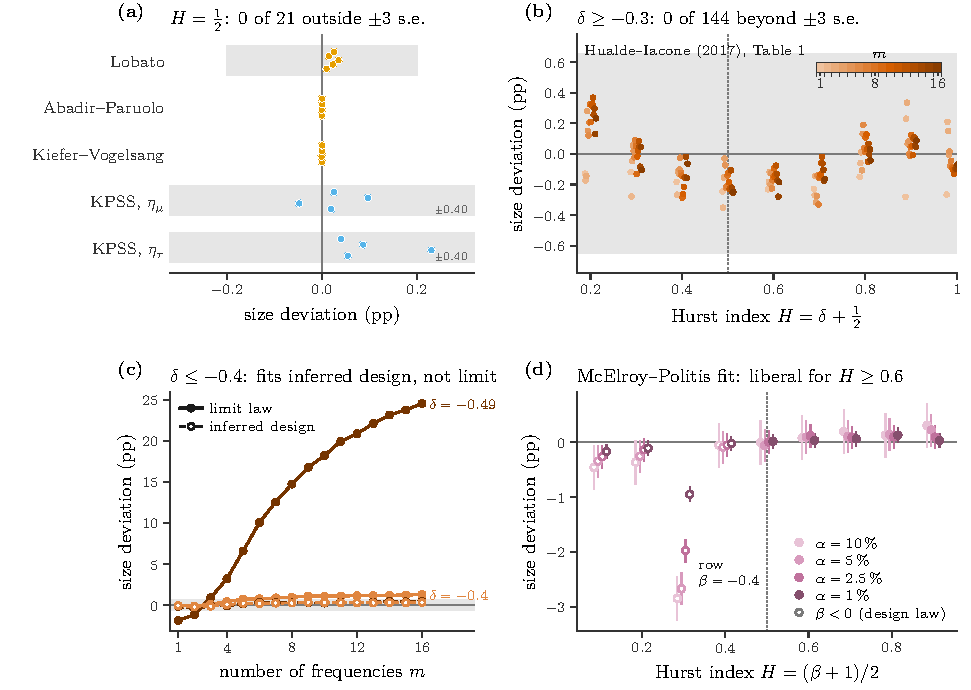
\includegraphics[width=\textwidth]{fig4_audit.pdf}
\caption{Size deviation of published critical values (pp); grey: $\pm3$ Monte Carlo standard errors of each
source's design. (a)~Sources at $H=\frac12$. (b)~\citet[Table~1]{HI17}, $\delta\ge-0.3$. (c)~Same table,
$\delta=-0.49$, $-0.4$: limit (filled), inferred finite design (open). (d)~\citet{MP09}: limit (filled), their
design (open); bars: $\pm3$ raw-quantile standard errors (reference scale, not a bound).}\label{fig:audit}
\end{figure}

\paragraph{$H=\frac12$} The values of \citet{AP97} and \citet{KV02} are exact to the printed digits: the largest
relative difference from the closed-form quantiles is \pthree{audit-apkv-maxrel}. The row $K=1$ of \citet[Table~1]{Lob01}
delivers sizes \pthree{audit-lob-sizes}\,\% at nominal $10$, $5$, $2.5$, $1$ and $0.5\,\%$, all within the Monte Carlo
error of the published design. For the stationarity statistics of \citet{KPSS92}, a bridge functional at $H=\frac12$,
the values for $\eta_\mu$ are accurate within Monte Carlo error, while the $5\,\%$ value $0.146$ for $\eta_\tau$ has size
\pthree{audit-kpss-tau-05}\,\%, \pthree{audit-kpss-tau-05-z} standard errors above nominal; the exact $5\,\%$ point is
\pthree{audit-kpss-tau-05-exact}.

\paragraph{Fixed-$m$ values of \citet{HI17}} Their Table~1 gives $176$ two-sided $5\,\%$ values for
$\delta=H-\frac12\in[-0.49,0.49]$ and $m=1,\dots,16$, from $10\,000$ replications in which the integrals of the limit
are replaced by sums over $10\,000$ steps (their Remark~6). For $\delta\ge0$ the true sizes range from
\pthree{audit-hi-pos-min} to \pthree{audit-hi-pos-max}\,\%; none of the \pthree{audit-hi-pos-n} values is more than two
standard errors from $5\,\%$, but \pthree{audit-hi-pos-gt01} of them miss $5\,\%$ by more than $0.1$\,pp. At $\delta=0$,
where the limit law is Student's $t$ with $2m$ degrees of freedom, all \pthree{audit-D-hi0-n} values are conservative,
with sizes from \pthree{audit-D-hi0-min} to \pthree{audit-D-hi0-max}\,\% (largest $|z|$ \pthree{audit-D-hi0-maxz}); their
standardised sum is \pthree{audit-D-hi0-jointz} (class~D), but the sixteen values share the replications of one
simulation, and treated as a single observation the row deviates by \pthree{audit-D-hi0-rowz} standard errors. For $\delta<0$,
certified through \cref{prop:continuation}, the limit sizes range from \pthree{audit-hi-neg-min} to
\pthree{audit-hi-neg-max}\,\%, and \pthree{audit-hi-neg-gt3se} of the \pthree{audit-hi-neg-n} values are more than three
standard errors from $5\,\%$ (\pthree{audit-hi-neg-gt2se} more than two). All of these are at $\delta=-0.49$ and $-0.4$, where the deviation grows with $m$: at
$\delta=-0.49$ the published value for $m=1$ has limit size \pthree{audit-hi-neg-m1-limit}\,\% and the one for $m=16$
has \pthree{audit-hi-neg-m16-limit}\,\%. The published values are nevertheless consistent with a finite design that could
have produced them. Under the exact law of the statistic computed from a stationary ARFIMA$(0,\delta,0)$ path of $10\,000$
observations, their sizes range from \pthree{audit-hi-neg-design-min} to \pthree{audit-hi-neg-design-max}\,\%, only
\pthree{audit-hi-neg-design-gt2} of the $80$ values are more than two standard errors from $5\,\%$, and none is more than
three (largest $|z|$ \pthree{audit-hi-neg-design-maxz}); a fractional Gaussian noise path of the same length gives
\pthree{audit-hi-neg-m16-fgn}\,\% at $\delta=-0.49$, $m=16$, close to the limit. Near $\delta=-\frac12$ the discretised
law approaches its limit extremely slowly: at $\delta=-0.49$ and $m=16$ the published value has size
\pthree{audit-hi-neg-m16-T1e3}, \pthree{audit-hi-neg-m16-T1e4} and \pthree{audit-hi-neg-m16-T1e5}\,\% for ARFIMA paths
of $10^3$, $10^4$ and $10^5$ observations. Their Remark~6 gives the number of steps but not the process that generated
the increments; the ARFIMA design is our inference from this match, so class~C is a statement about an inferred design.
The values are accurate for that design but are not limit critical values, and for strongly antipersistent series the critical value
must be taken from the exact finite-sample law at the actual $n$ (\cref{prop:exactn}). For $\delta\ge-0.3$ the table is
accurate to its Monte Carlo precision of about $\pm$\pthree{audit-hi-2se}\,pp in size, which is larger than the effect
of $\delta$ on the critical value at small $|\delta|$; the certified values replace it (\cref{app:tables}).

\paragraph{Bartlett values of \citet{MP09}} McElroy and Politis do not print simulated quantiles: for each kernel and
memory parameter $\beta=2H-1$ they print the coefficients of a polynomial fit of the $\log$ critical value in the
bandwidth ratio $b$. The Bartlett values at $b=1$ that we audit are therefore \emph{fitted values}, reconstructed from
the printed coefficients as $\exp(\sum_ia_i)$, and the error of the fit is part of what is measured. As the reference
scale we use the standard error of a raw simulated quantile at their $N=50\,000$; the uncertainty of a fitted value can
be smaller, because the fit pools neighbouring values of $b$, or larger, because the fit may be biased at the end point
$b=1$. At $H=\frac12$ the fitted
values deliver sizes within Monte Carlo error. For $H\ge0.6$ all \pthree{audit-mp-pos-n} values are too small: each is
within three standard errors (largest $z$ \pthree{audit-mp-pos-maxz}), but all \pthree{audit-mp-pos-npos} excesses are
positive, between \pthree{audit-mp-pos-min} and \pthree{audit-mp-pos-max}\,pp, and at $H=0.9$ and nominal $10\,\%$ the
size is \pthree{audit-mp-H090-a10}\,\% (class~D, standardised sum \pthree{audit-D-jointz}). The four levels of a row are
quantiles of one simulated sample; counting each of the \pthree{audit-D-nrows} rows as one observation, the excess is
\pthree{audit-D-jointz-rows} standard errors, so the pattern is suggestive rather than established. The excess does not
come from discretisation, because the exact law of
their $1000$-step design gives the same sizes; it may come from the polynomial smoothing at the end point $b=1$, which
we cannot verify from the report. For $\beta<0$ we compare with the exact finite-sample law of their discretised
design. The row $\beta=-0.4$ ($H=0.3$) is inaccurate: its size deviations reach \pthree{audit-mp-T3-dev10}\,pp at
nominal $10\,\%$, the size at nominal $5\,\%$ is \pthree{audit-mp-T3-size05}\,\%, and the deviations are up to
\pthree{audit-mp-T3-maxz} standard errors; the row is also non-monotone in $\beta$ at the upper levels, which is consistent with, but not proof of, a
transcription error in one printed coefficient; the report does not allow us to check this. Rounding of the printed
coefficients to three decimals does not explain it: it moves the size by at most \pthree{audit-mp-T3-round-maxshift}\,pp,
against deviations of \pthree{audit-mp-T3-round-mindev}\,pp and more. The row $\beta=-0.8$ deviates by \pthree{audit-mp-T1-devmin} to
\pthree{audit-mp-T1-devmax}\,pp, \pthree{audit-mp-T1-minz}--\pthree{audit-mp-T1-maxz} standard errors (class~E,
conservative); the rows $\beta=-0.6$ and $-0.2$ are within Monte Carlo error.

\paragraph{Summary} Of the \pthree{audit-n-values} audited values (the \pthree{audit-n-dup} values of the 1990 KPSS working
paper, identical to those of the article, are counted once), \pthree{audit-n-AB} are within three standard errors
of nominal in the law they are meant for (classes A and B), \pthree{audit-n-C} are consistent with a finite design that
we infer their source simulated but not with the limit (C), \pthree{audit-n-D} share a one-sign pattern within Monte
Carlo error (D), and
\pthree{audit-n-E} are more than three standard errors from nominal (E), all of them fitted McElroy--Politis values
at $\beta<0$; \cref{tab:audit} lists the classes by source and \cref{app:audit} every value. Two messages follow for the
user of a table. Monte Carlo precision of $\pm0.2$ to $\pm0.4$\,pp in size is all that most published tables deliver,
and \pthree{audit-n-B} values miss $5\,\%$ by more than $0.1$\,pp for that reason alone. And for the long-memory tables
the systematic component, whether from the fit or from the simulated design, can be larger than the Monte Carlo error.

\begin{table}[tbp]\centering\small
\caption{Verdicts by source. Deviation: true size minus nominal (pp); s.e.: Monte Carlo standard error of the
source's design; classes as in the text. \textsuperscript{a}No Monte Carlo error. The 1990 KPSS working paper,
identical to the article, is counted once.}\label{tab:audit}
\begin{tabular}{@{}llrrrrrrrr@{}}\toprule
& & & & & \multicolumn{5}{c}{verdict class}\\\cmidrule(l){6-10}
source & range & $N$ & deviation (pp) & s.e.\ (pp) & A & B & C & D & E\\\midrule
Lobato~\fixcite{Lob01} & $H=\frac12$ & 5 & +0.01 to +0.03 & 0.02--0.07 & 5 & -- & -- & -- & --\\
Abadir--Paruolo~\fixcite{AP97} & $H=\frac12$ & 4 & -0.00 to +0.00 & exact\textsuperscript{a} & 4 & -- & -- & -- & --\\
Kiefer--Vogelsang~\fixcite{KV02} & $H=\frac12$ & 4 & -0.00 to +0.00 & exact\textsuperscript{a} & 4 & -- & -- & -- & --\\
KPSS~\fixcite{KPSS92} & $H=\frac12$ & 8 & -0.05 to +0.23 & 0.04--0.13 & 7 & 1 & -- & -- & --\\
Hualde--Iacone~\fixcite{HI17} & $\delta\ge0$ & 96 & -0.35 to +0.34 & 0.22 & 36 & 44 & -- & 16 & --\\
Hualde--Iacone~\fixcite{HI17} & $\delta<0$ & 80 & -1.87 to +24.53 & 0.22 & 16 & 36 & 28 & -- & --\\
McElroy--Politis~\fixcite{MP09} & $\beta\ge0$ & 20 & -0.06 to +0.31 & 0.04--0.13 & 4 & -- & -- & 16 & --\\
McElroy--Politis~\fixcite{MP09} & $\beta<0$ & 16 & -2.85 to -0.02 & 0.04--0.13 & 7 & 1 & -- & -- & 8\\
\midrule all & & 233 & & & 83 & 82 & 28 & 32 & 8\\
\bottomrule\end{tabular}
%
\end{table}
%
\section{Computation and certification with \CosCert}\label{sec:computation}

\subsection{A certified distribution function for \texorpdfstring{$T_H$}{T\_H}}
Write $F_H(c)=P(T_H\le c)=P(Z^2-c\,D_{\SN}\le0)$. By \cref{prop:coords}, $D_{\SN}=W_J+R_J$ with
$W_J=\sum_{k\le J}\Lambda_k^2/(k\pi)^2$, a quadratic form in the $(J+1)$-dimensional Gaussian vector
$(Z,\Lambda_1,\dots,\Lambda_J)$ with closed-form covariance, and the remainder $R_J\ge0$ of \cref{thm:eig}. Let
$X_J=Z^2-cW_J$ and $\bar\mu_J=\min(\tau_J,\bar c_J)$.

\begin{theorem}[Certified enclosure]\label{thm:certificate}
Let $\frac12\le H<1$, $c>0$, $J\ge1$, $t>0$, and
$s_{\mathrm{hi}}=\tau_J+2\sqrt{\bar\mu_J\tau_Jt}+2\bar\mu_Jt$, $s_{\mathrm{lo}}=\max(0,\tau_J-2\sqrt{\bar\mu_J\tau_Jt})$. Then
\[P(X_J\le c\,s_{\mathrm{lo}})-e^{-t}\;\le\;F_H(c)\;\le\;P(X_J\le c\,s_{\mathrm{hi}})+e^{-t}.\]
For every $x$, every $\Delta>0$ and every tilt $\vartheta\in(0,\frac12)$, the exceedance probability satisfies
\[\big|P(X_J>x)-S_{\Delta,K}(x)\big|\le\epsilon_\Delta^+(x)+\epsilon_\Delta^-+\epsilon_K,\]
where $S_{\Delta,K}$ is the sum of the first $K$ terms of the tilted midpoint sum $S_\Delta$ of the inversion integral,
$\epsilon_\Delta^\pm$ bound the upper and lower aliases of $S_\Delta$ and $\epsilon_K$ the omitted terms, all given
explicitly in the proof (\cref{app:proofs}) and \cref{app:certificate}; hence $P(X_J\le x)=1-P(X_J>x)$ is enclosed by an interval of the same width. With $x=c\,s_{\mathrm{lo}}$ and
$x=c\,s_{\mathrm{hi}}$ the two statements together give a computable enclosure of $F_H(c)$.
\end{theorem}

The theorem reduces the infinite-dimensional problem to a finite one with explicit, rigorous error terms: the
remainder enters only through $\tau_J$, which is a closed form, and $\bar c_J$ from \cref{thm:eig}; the remainder's
dependence on $(Z,W_J)$ never needs to be known. The finite problem is solved in ball arithmetic \citep{Joh17}.
The characteristic function of $X_J$ is evaluated without an eigendecomposition of the $(J+1)$-dimensional covariance:
the odd cosine coordinates are uncorrelated with the rest (\cref{prop:coords}c), so the determinant factorises into an odd block, an even block and a scalar Schur
complement carrying $Z$; each factor is evaluated as a head block of up to $128$ coordinates, diagonalised approximately in floating point and
corrected by an exact similarity transformation in ball arithmetic, and a tail block bounded through its trace,
Frobenius norm and couplings.
The principal branch of every square root is the correct one on the whole strip $0\le\operatorname{Re}z<\frac12$
(\cref{lem:branch}): the scalar factor carrying $Z$, $r(z)=1-2z\,s^\top(I+2zB)^{-1}s$, has
$\operatorname{Im}r(\vartheta+\mathrm it)=-2t\sum_js_j^2/|1+2zb_j|^2$ and $r(\vartheta)\ge1-2\vartheta$, so it never meets the
cut $(-\infty,0]$. Critical values follow by bracketing: if the certified lower bound of $F_H$ at $q^+$ exceeds $p$ and
the certified upper bound at $q^-$ falls below $p$, then $q_p\in[q^-,q^+]$.

All production values use $J=16384$ and $t=25$, so that each of the two exceptional probabilities is $e^{-25}<1.4\times10^{-11}$.
The protocol fixed these choices before production, after a benchmark over $J=512,\dots,16384$ (\cref{fig:certificate}b):
the width of the enclosure decreases like $J^{-1/2-2H}$, as \cref{prop:rate} below predicts (the measured local slopes
differ from $-\frac12-2H$ by at most \pthree{e1-slope-maxdev} for $J\le8192$), and at $J=16384$ it is at most
\pthree{e1-width-max-16384} in probability. For $H\ge0.95$ the last doubling of $J$ gains less, because the
finite-dimensional radius, which does not decrease with $J$, is reached. The tilted inversion
($\vartheta=\frac14$) needs \pthree{e1-tilt-node-ratio-min}--\pthree{e1-tilt-node-ratio-max} times fewer nodes than the
untilted one at the same accuracy.

The rate of the enclosure, and what it depends on, can be stated precisely.

\begin{proposition}[Width of the enclosure]\label[proposition]{prop:rate}
Let $\frac12\le H<1$, $c>0$, $t\ge1$, $J_0\ge4$, and let $\alpha_2\ge\alpha_3\ge\alpha_4$ be the second to fourth largest
eigenvalues of the covariance of $(\Lambda_k/(k\pi))_{k\le J_0}$. For every $J\ge J_0$ with $\tau_J\ge4\bar c_Jt$, the
interval of the first statement of \cref{thm:certificate} has width
\[w_J\le c\bar f\big(4\sqrt{\bar c_J\tau_Jt}+2\bar c_Jt\big)+2e^{-t},\qquad
\bar f=\frac1{2\pi}\int_{\mathbb R}\prod_{i=2}^4\big(1+4c^2\alpha_i^2s^2\big)^{-1/4}\dd s<\infty .\]
Since $\tau_J\asymp J^{-2H}$ and $\bar c_J\asymp J^{-1-2H}$, $w_J-2e^{-t}=O(\sqrt t\,J^{-1/2-2H})$, where
$t=\log(1/p)$ for a failure probability $p$. The computed enclosure adds the numerical radii of \cref{app:certificate},
which do not decrease with $J$, and a quantile bracket has width close to $w_J/f_H(q)$.
\end{proposition}

\begin{figure}[tbp]\centering
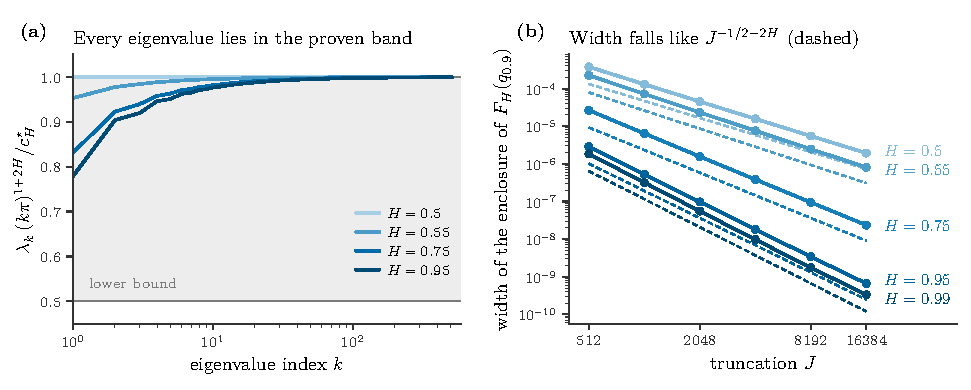
\includegraphics[width=\textwidth]{fig6_certificate.pdf}
\caption{Spectrum and certificate of the fractional Brownian bridge. (a)~Eigenvalues relative to the upper bound of
\cref{thm:eig} (Galerkin, $J=2048$); the lower bound is $\frac12$. (b)~Width of the certified enclosure of $F_H$ at the
$90\,\%$ quantile against $J$; dashed: slope $-\frac12-2H$ (\cref{prop:rate}), offset for visibility.}\label{fig:certificate}
\end{figure}

\subsection{Computational methods on identical targets}\label{sec:methods}
We compared \pthree{e5-n-impl} implementations and modes of \pthree{e5-n-methods} distinct methods for generalized
chi-square probabilities on four targets: a fixed-$m$ limit (T1, $m=8$, $H=0.8$), an EWC limit (T2, $B=16$, $H=0.8$),
the exact finite-sample law of $T_n$ at $n=1000$ under ARFIMA$(0,0.2,0)$ (T3), and the limit law of $T_H$ at $H=0.75$
(T4). Every method received the same weights. The covariance of the fixed-smoothing coordinates is a shared input;
beyond it, each method is charged the spectral step it needs, the certified enclosure its enclosure of the weights and
the double-precision methods a Cholesky factorisation and the eigenvalues of the ratio form, which depend on the cutoff.
Against a certified enclosure $[L,U]$ a computed value $v$ has a true error in
$[\operatorname{dist}(v,[L,U]),\max(|v-L|,|v-U|)]$, and we report this interval; on T3 the reference is the computed
exact law of \cref{prop:exactn}(b), which the Imhof and Bromwich implementations confirm to $10^{-13}$. A method used
outside its documented domain is run and labelled but not compared: the approximation of \citet{LTZ09} is documented
for non-negative definite forms, and all four targets are indefinite. The R methods for positive forms, those of
\citet{Hal83} and \citet{BE88} (HBE) and \citet{LPB00} (LPB4) as implemented by \citet{BA16}, and the saddlepoint and
\citet{Sat46} options of the survey package \citep{Lum04}, are applied to the negative part of the form and integrated
over the positive one by adaptive quadrature; a $64$-node Gauss--Hermite rule, which does not resolve the kink of that
integrand, changes their values by up to \pthree{e5-gh-maxdiff-pp}\,pp.

\begin{figure}[tbp]\centering
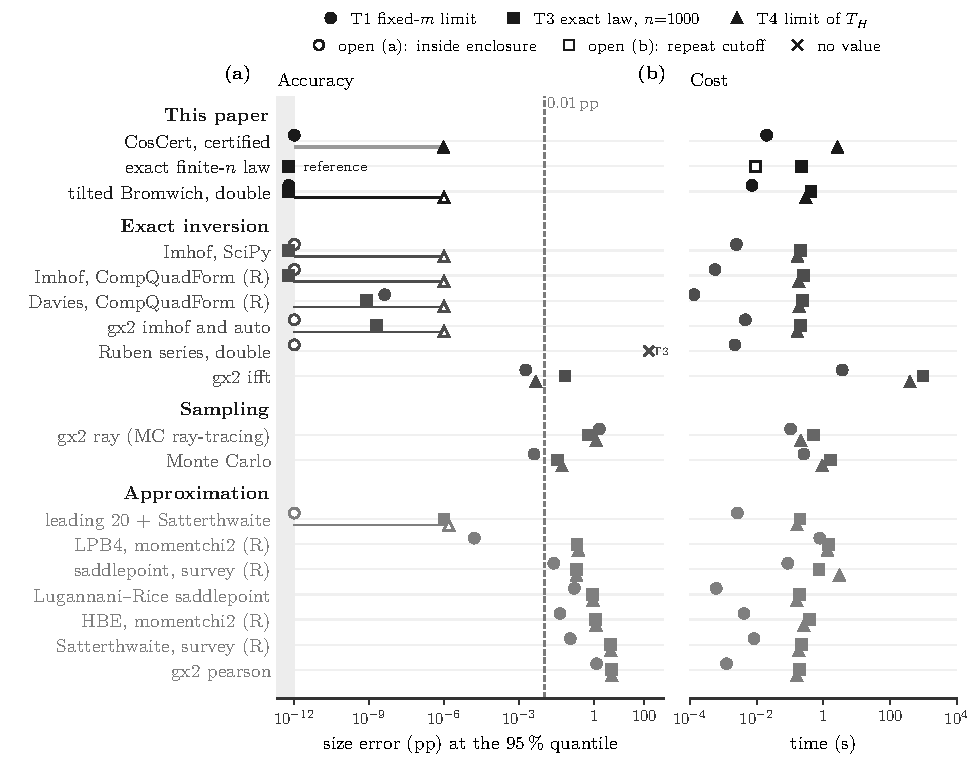
\includegraphics[width=\textwidth]{fig5_methods.pdf}
\caption{Accuracy and cost of computational methods on identical targets (T1, T3, T4; \cref{sec:methods}). (a)~Size
error at the $95\,\%$ quantile; open markers: upper bounds (value inside the certified enclosure); grey bars: certified
half-widths; shaded: double-precision floor. (b)~Wall-clock time including each method's spectral step.}\label{fig:methods}
\end{figure}

Three conclusions follow. First, on the low-rank targets T1 and T2 every exact inversion method, Imhof's integral in
three implementations (SciPy, the R package of \citet{DL10}, and the \texttt{imhof} and \texttt{auto} modes of
\citet{Das25}), Davies' algorithm, Ruben's series and our tilted Bromwich rule, has error at most
\pthree{e5-T12-exact-maxerr} in probability at a cost below \pthree{e5-T12-exact-maxs}\,s, and the certified enclosure,
of width \pthree{e5-T12-cert-width}, costs \pthree{e5-T12-cert-s}\,s. Second, the approximations are not accurate enough
for critical values. At the $5\,\%$ level the saddlepoint approximation of \citet{Kuo99} errs by up to
\pthree{e5-lr-err-pp}\,pp in size, HBE by \pthree{e5-hbe-err-pp}, the saddlepoint option of survey by
\pthree{e5-svsaddle-err-pp}, LPB4 by \pthree{e5-lpb4-err-pp} and Satterthwaite's two-moment approximation by
\pthree{e5-satt-err-pp}\,pp; Pearson's three-moment approximation (the \texttt{pearson} mode of \citet{Das25}) errs by
\pthree{e5-3mom-T1-pp}\,pp on T1 and returns the probability $1$ on T3 and T4, an error of
\pthree{e5-approx-maxerr-pp}\,pp. A hybrid of the type studied by \citet{CL19}, which keeps the $20$ largest weights exactly and replaces
the others by a two-moment scaled chi-square with fractional degrees of freedom, is accurate to
\pthree{e5-lead20-err} in probability on every target. Third, for the long-memory targets the cost is the spectral step.
On T3 the exact law of \cref{prop:exactn}(b) pays \pthree{e5-T3-setup-s}\,s once, for one Cholesky factorisation and one
eigendecomposition, and then \pthree{e5-T3-query-s}\,s per cutoff, whereas a method that needs the eigenvalues of the
cutoff-dependent ratio form pays \pthree{e5-T3-eig-s}\,s for them at every cutoff (\pthree{e5-T3-imhof-s}\,s in all with
Imhof's integral). For one cutoff the costs are comparable; over \pthree{e5-amort-m} cutoffs they are
\pthree{e5-amort-ours-s}\,s and \pthree{e5-amort-imhof-s}\,s, with agreement to \pthree{e5-amort-maxdiff}. The
\texttt{ifft} mode of \citet{Das25} took \pthree{e5-T3-ifft-s}\,s on T3 and was less accurate, and on T4 with $J=2048$
it exceeded the available memory; the \texttt{ray} mode took \pthree{e5-T4-ray2048-s}\,s there. On T4, Imhof's
integral on the $J=512$ cosine coordinates, with the remainder replaced by its mean, lies inside the certified
enclosure, of width \pthree{e5-T4-ref-width}, so its error is at most \pthree{e5-T4-galerkin-err}; it takes
\pthree{e5-T4-galerkin-s}\,s against \pthree{e5-T4-cert-s}\,s for the certified evaluation at $J=16384$, including the
construction of the system. We recommend it whenever a guarantee is not needed, and use the certificate to confirm it.
All times are wall-clock times on one machine (\pthree{e5-env}, single-threaded linear algebra) and indicate orders of
magnitude only.
%
\FloatBarrier
\section{Recommendations}\label{sec:conclusion}

For a test of the mean under long memory we recommend the following.
\begin{enumerate}
\item Use critical values for the value of $H$ at hand. Short-memory values are invalid under long memory: at $H=0.9$
the nominal $5\,\%$ tests reject a true null between \pthree{naive-min-0.90} and \pthree{naive-max-0.90}\,\% of the time
(\cref{fig:headline}). In the three applications, changing the cutoff changes some decisions and widens nominal
confidence intervals by up to \pthree{emp-nile-HI16-ratio} times (\cref{sec:empirical}).
\item Take critical values from Supplementary Material Tables~S.1--S.2 or the accompanying archive, or, for
fixed-smoothing tests, from the closed-form rule \eqref{eq:rescaled}, whose size error is at most
\pthree{rs-maxerr-090-0.05}\,pp at $5\,\%$ for the tabulated $H\le0.9$ and every tabulated $m\le16$ and $B\le32$. For the
Bartlett/self-normalised test use \cref{tab:sncv} or the response surface checked at held-out grid points of \cref{tab:surface}; the rescaling
rule does not apply to it.
\item Prefer a fixed-smoothing test with few components, $m\le4$ frequencies or $B\in\{4,8\}$ cosines: with the
correct critical value it is within \pthree{fn-maxdev-small-100}\,pp of $5\,\%$ from $n=100$ in every design studied. With
$m=4$ ($B=8$) its limit power exceeds that of the Bartlett/self-normalised test at every $H$ and local alternative of
our grid (\cref{sec:power}); use more components only when $n$ is large or short-run dynamics are known to be weak.
\item Account explicitly for uncertainty in $\hat H$. With a raw local Whittle estimate, nominal $5\,\%$ tests reject
\pthree{pl-pure-min-100}--\pthree{pl-pure-max-100}\,\% of the time at $n=100$ even without short-run dynamics
(\cref{tab:plugin}), while the critical-value error itself is negligible (below \pthree{sn-print-maxerr}\,pp for the printed Bartlett values). For HI with $m=4$, ELW brought size closer to nominal in \pthree{comp-elw-closer}
of the 24 designs. The upper-confidence rule reduced both size and power. Even with that rule, the simulated
rejection rate reached \pthree{comp-up-worst}\,\% at $n=100$ (\cref{sec:competitors}).
\item When comparing with earlier tables, match the normalisation and tail of the statistic (\cref{tab:norm}) first.
Published simulation tables deliver Monte Carlo precision of a few tenths of a percentage point in size; for strongly
antipersistent series ($\delta\le-0.4$) the fixed-$m$ values of \citet{HI17} reflect an inferred finite design rather
than the limit, and practitioners should compute exact finite-$n$ laws directly via \cref{prop:exactn}.
\end{enumerate}
\CosCert{} extends to other functionals of the same cosine coordinates, such as the stationarity statistics of
\citet{KPSS92} under long memory; at $H=\frac12$ it already reproduces the Cram\'er--von Mises law of $\eta_\mu$
(Supplementary Material Table~S.9). We leave these extensions to future work.
%

\section*{Data and code availability}
The code, empirical datasets, numerical results and manuscript sources supporting this study are publicly available at
\url{https://github.com/EslamAhmedGaber/CosCert} and in the supplementary archive
\texttt{CosCert\_\allowbreak code\_\allowbreak and\_\allowbreak data.zip}; Supplementary Material Section~S.4 explains
how every number, figure and table is rebuilt from them.

\section*{CRediT authorship contribution statement}
\textbf{Eslam Ahmed:} Conceptualization, Methodology, Software, Formal analysis, Investigation, Validation, Visualization, Writing -- original draft, Writing -- review \& editing.
\textbf{Mohamed A. El-Beltagy:} Conceptualization, Methodology, Formal analysis, Supervision, Writing -- review \& editing.
\textbf{Ahmed Etman:} Writing -- review \& editing.
\textbf{Sroor M. Elnady:} Writing -- review \& editing.

\section*{Declaration of competing interest}
The authors declare that they have no known competing financial interests or personal relationships that could have appeared to influence the work reported in this paper.

\section*{Acknowledgements}
The authors acknowledge support from the Science, Technology \& Innovation Funding Authority (STDF), Egypt, under the Basic Sciences Grant (Project ID 50925). The funder had no role in the study design, analysis and interpretation, manuscript preparation or decision to submit the work for publication.

\section*{Declaration of generative AI and AI-assisted technologies in the manuscript preparation process}
During the preparation of this work the authors used ChatGPT (including Codex) and Claude to revise the prose, document the code and assist with numerical and editorial checks. After using these tools, the authors reviewed and edited the content as needed and take full responsibility for the content of the published article.

\bibliographystyle{elsarticle-num-names}
\bibliography{references}

\appendix
\crefalias{section}{appendix}
\section{Proofs}\label{app:proofs}

Throughout, $R(s,t)=\frac12(s^{2H}+t^{2H}-|t-s|^{2H})$, $b=2H-1$, and for $f\in C^1[0,1]$ the Wiener integral is
\begin{equation}\label{eq:ibp}
\int_0^1f\dd B_H=f(1)B_H(1)-\int_0^1f'(r)B_H(r)\dd r ,
\end{equation}
which agrees with the $L^2$ extension of the integral of step functions for every $0<H<1$ \citep{PT00}. For
$\frac12<H<1$ and $f,g\in L^2(0,1)$, $\E[\int f\dd B_H\int g\dd B_H]=Hb\int_0^1\!\int_0^1f(u)g(v)|u-v|^{b-1}\dd u\dd v$
\citep{PT00}. We write $p_k+\mathrm ir_k={}_1F_1(b;b+1;\mathrm ik\pi)=b\int_0^1x^{b-1}e^{\mathrm ik\pi x}\dd x$ ($b>0$).

\subsection{Proof of \texorpdfstring{\cref{prop:coords}}{Proposition 1}}
\emph{(a)} Let $e_k(r)=\sqrt2\sin(k\pi r)$ and $E_k(r)=-\sqrt2\cos(k\pi r)/(k\pi)$, so $E_k'=e_k$. The path $\Bt$ is
continuous with $\Bt(0)=\Bt(1)=0$, and \eqref{eq:ibp} applied to $\Bt=B_H-rZ$ gives
\[\int_0^1\Bt e_k\dd r=-\int_0^1E_k\dd\Bt=\frac1{k\pi}\Big(\int_0^1\sqrt2\cos(k\pi r)\dd B_H(r)-Z\int_0^1\sqrt2\cos(k\pi r)\dd r\Big)
=\frac{\Lambda_k}{k\pi},\]
because $\int_0^1\cos(k\pi r)\dd r=0$ for $k\ge1$. Since $(e_k)_{k\ge1}$ is an orthonormal basis of $L^2(0,1)$,
Parseval's identity gives $\int\Bt^2=\sum_k\Lambda_k^2/(k\pi)^2$ for every path; the partial sums increase, so the
convergence also holds in $L^1$ by monotone convergence.

\emph{(b)} $C_j=\int\cos(2\pi jr)\dd B_H=\Lambda_{2j}/\sqrt2$ and $S_j=\Sigma_{2j}/\sqrt2$ by definition; insert into
\eqref{eq:limits}.

\emph{(c)} For $\frac12\le H<1$ this is \citet[Proposition~1, closed-form Gram matrices]{AhmedCosChaos}; for $0<H<\frac12$ see
\cref{prop:continuation}.

\emph{Parity.} The process $B'(r)=B_H(1)-B_H(1-r)$ is again a Type~I fractional Brownian motion, and for step functions,
hence for all integrands, $\int f\dd B'=\int f(1-u)\dd B_H(u)$. Since $\cos(k\pi(1-u))=(-1)^k\cos(k\pi u)$ and
$\sin(k\pi(1-u))=(-1)^{k+1}\sin(k\pi u)$, the joint law of $(Z,(\Lambda_k),(\Sigma_k))$ is invariant under
$(Z,\Lambda_k,\Sigma_k)\mapsto(Z,(-1)^k\Lambda_k,(-1)^{k+1}\Sigma_k)$. Hence
$\Cov(\Lambda_k,\Lambda_l)=(-1)^{k+l}\Cov(\Lambda_k,\Lambda_l)$, $\Cov(\Sigma_k,\Sigma_l)=(-1)^{k+l}\Cov(\Sigma_k,\Sigma_l)$
and $\Cov(\Sigma_i,\Lambda_k)=(-1)^{i+k+1}\Cov(\Sigma_i,\Lambda_k)$, which vanish when $k+l$ is odd, $k+l$ is odd and
$i+k$ is even, respectively.

\emph{(d)} Let $\frac12<H<1$ and $\kappa(w)=|w|^{b-1}$. With $u=(\sigma+w)/2$, $v=(\sigma-w)/2$ the unit square becomes
$\{|w|\le1,\ |w|\le\sigma\le2-|w|\}$ with $\dd u\dd v=\frac12\dd\sigma\dd w$. For integers $i,j\ge1$ put
$a=(i-j)\pi/2$ and $c=(i+j)\pi/2$, so $i\pi u-j\pi v=a\sigma+cw$ and $i\pi u+j\pi v=c\sigma+aw$, and let
\[I_1=\iint\cos(i\pi u-j\pi v)\kappa(u-v)\dd u\dd v,\qquad I_2=\iint\cos(i\pi u+j\pi v)\kappa(u-v)\dd u\dd v.\]
For $i\ne j$, integrating in $\sigma$ and using $\sin(n\pi-y)=(-1)^{n+1}\sin y$ with $n=i-j$, then combining $w=\pm x$,
\[I_1=\frac{1+(-1)^{i-j}}{2a}\int_0^1x^{b-1}\big(\sin(j\pi x)-\sin(i\pi x)\big)\dd x=\frac{1+(-1)^{i-j}}{(i-j)\pi}\,\frac{r_j-r_i}b,\]
and in the same way $I_2=-\frac{1+(-1)^{i+j}}{(i+j)\pi}\frac{r_i+r_j}b$. For $i=j$ the inner integrals give
$I_1=2\int_0^1x^{b-1}(1-x)\cos(i\pi x)\dd x$ and $I_2=-\frac{2r_i}{i\pi b}$. Integration by parts gives
$\int_0^1x^b\cos(k\pi x)\dd x=-r_k/(k\pi)$, hence $I_1=\frac2b\big(p_i+\frac{b\,r_i}{i\pi}\big)$. Since
$2\sin(i\pi u)\sin(j\pi v)=\cos(i\pi u-j\pi v)-\cos(i\pi u+j\pi v)$,
$\Cov(\Sigma_i,\Sigma_j)=Hb(I_1-I_2)$, which is the stated formula: for $i=j$,
$Hb\cdot\frac2b\big(p_i+\frac{(1+b)r_i}{i\pi}\big)$, and for $i\ne j$ with $i+j$ even,
$\frac{2H}\pi\big(\frac{r_i+r_j}{i+j}-\frac{r_i-r_j}{i-j}\big)=\frac{4H}\pi\frac{ir_j-jr_i}{i^2-j^2}$. (With
$2\cos\cos=\cos(\cdot-\cdot)+\cos(\cdot+\cdot)$ the same computation returns the cosine Gram matrix of
\cref{prop:coords}(c), an independent check.) At $H=\frac12$ both sides are continuous in $H$ (\cref{prop:continuation}),
and for $0<H<\frac12$ the formula holds by \cref{prop:continuation}.

\subsection{Proof of \texorpdfstring{\cref{prop:continuation}}{Proposition 2}}
By \eqref{eq:ibp}, $\Lambda_k=\sqrt2(-1)^kZ+\sqrt2k\pi\int_0^1\sin(k\pi r)B_H(r)\dd r$, so $\E\Lambda_k\Lambda_l$ is a
finite combination of $R(1,1)$, $\int_0^1\sin(l\pi r)R(1,r)\dd r$ and
$\int_0^1\!\int_0^1\sin(k\pi r)\sin(l\pi s)R(r,s)\dd r\dd s$; similarly for $\Sigma_k$ and for cross terms. For complex
$H$ with $0<\operatorname{Re}H<1$ and $r,s\in(0,1]$, $r\ne s$, the map $H\mapsto R(r,s)$ is holomorphic and
$|R(r,s)|\le\frac32$, because $|x^{2H}|=x^{2\operatorname{Re}H}\le1$ on $(0,1]$. By dominated convergence and Morera's
theorem the covariances are holomorphic in the strip, hence real-analytic on $(0,1)$. On the other side, the Kummer
series ${}_1F_1(b;b+1;z)=\sum_{n\ge0}\frac{b}{b+n}\frac{z^n}{n!}$ is holomorphic in $b$ away from
$b\in\{-1,-2,\dots\}$, i.e.\ for $\operatorname{Re}H>0$; so $p_k(H)$, $r_k(H)$ and the rational expressions of
\cref{prop:coords}(c)--(d) are real-analytic on $(0,1)$. The two real-analytic functions agree on $(\frac12,1)$, hence
on $(0,1)$ by the identity theorem. \qed

\subsection{Proof of \texorpdfstring{\cref{thm:eig}}{Theorem 3}}
In the basis $(e_k)$ the operator $K_{\mathrm{br}}$ has the matrix $M_{kl}=\E\big[\int\Bt e_k\int\Bt e_l\big]=G_{kl}/(k\pi\,l\pi)$
by \cref{prop:coords}. \Citet[Lemma~3, two-sided weighted cosine inequality]{AhmedCosChaos} states, for $\frac12\le H<1$ and real square-summable
$(a_k)_{k\ge1}$, $\frac12\sum_kw_ka_k^2\le\sum_{k,l}a_ka_lG_{kl}\le\sum_kw_ka_k^2$ with $w_k=\cH(k\pi)^{1-2H}$ (the
case $T=1$; the inequality is stated for finite sums and extends to $\ell^2$ by continuity of both sides). Put
$a_k=x_k/(k\pi)$: then $\frac12x^\top Dx\le x^\top Mx\le x^\top Dx$ for all $x\in\ell^2$, with
$D=\operatorname{diag}(d_k)$, $d_k=\cH(k\pi)^{-1-2H}$ decreasing. By the Courant--Fischer min--max characterisation of the
eigenvalues of the compact positive operators $M$ and $D$, $\frac12d_k\le\lambda_k(M)\le d_k$. The covariance of
$(\Lambda_k/(k\pi))_{k>J}$ is the compression $M_{>J}$ (the first omitted mode is $k=J+1$, because by
\cref{prop:coords}(a) the $k$-th sine coefficient of the bridge is $\Lambda_k/(k\pi)$ and $W_J$ contains $k\le J$), for which $x^\top M_{>J}x\le\sum_{k>J}d_kx_k^2\le d_{J+1}|x|^2$, so
its eigenvalues, which are the coefficients of $R_J$ in its Karhunen--Lo\`eve expansion $R_J\overset d=\sum_i\mu_i\xi_i^2$,
are at most $\bar c_J=d_{J+1}$. Finally $\E R_J=\sum_{k>J}M_{kk}=\tr K_{\mathrm{br}}-\sum_{k\le J}G_{kk}/(k\pi)^2$ and
$\tr K_{\mathrm{br}}=\int_0^1\Var\Bt(r)\dd r=\int_0^1\big(r^{2H}-r(r^{2H}+1-(1-r)^{2H})+r^2\big)\dd r
=\frac2{(2H+1)(2H+2)}-\frac16$, using $\int_0^1r(1-r)^{2H}\dd r=\frac1{(2H+1)(2H+2)}$. \qed

\subsection{Proof of \texorpdfstring{\cref{prop:rho}}{Proposition 4}}
$\E D_{\SN}=\tr K_{\mathrm{br}}$, which is $\frac16$ at $H=\frac12$; $\E D_{\HI,m}=m^{-1}\sum_j(\E C_j^2+\E S_j^2)
=(2m)^{-1}\sum_j(G_{2j,2j}+\Cov(\Sigma_{2j},\Sigma_{2j}))$ and $\E D_{\EWC,B}=B^{-1}\sum_jG_{jj}$, both equal to one at
$H=\frac12$ where $G$ and the sine Gram matrix are identities. Analyticity follows from \cref{prop:continuation}. As
$H\uparrow1$, $\E|B_H(r)-rZ|^2=r^{2H}-r(r^{2H}+1-(1-r)^{2H})+r^2\to0$ uniformly in $r$, so by \eqref{eq:ibp}
$\Lambda_k\to\sqrt2(-1)^kZ+\sqrt2k\pi Z\int_0^1r\sin(k\pi r)\dd r=0$ and
$\Sigma_{2j}\to-2\sqrt2j\pi Z\int_0^1r\cos(2j\pi r)\dd r=0$ in $L^2$; hence $\rho_P\to0$. The expansion of $\rho_{\SN}$
follows from $\frac{\dd}{\dd H}\frac6{(2H+1)(H+1)}\big|_{H=1}=-\frac76$. \qed

\subsection{Proof of \texorpdfstring{\cref{prop:edge}}{the growth proposition}}
Write $\varepsilon=1-H$, $K_H(r,s)=\Cov(\Bt(r),\Bt(s))$ and $R_H(r,s)=\frac12(r^{2H}+s^{2H}-|r-s|^{2H})$, so that
$K_H(r,s)=R_H(r,s)-sR_H(r,1)-rR_H(1,s)+rsR_H(1,1)$. At $H=1$, $K_1\equiv0$. Since $\partial_Hx^{2H}=2x^{2H}\log x$ and
$\partial_H^2x^{2H}=4x^{2H}(\log x)^2$ are bounded on $[0,1]\times[\frac12,1]$, Taylor's theorem gives
$\sup_{r,s}|K_H(r,s)/\varepsilon-k_1(r,s)|=O(\varepsilon)$ with $k_1=-\partial_HK_H|_{H=1}$ as stated; on the diagonal
$k_1(r,r)=-2r(1-r)\{r\log r+(1-r)\log(1-r)\}$, and $\int_0^1k_1(r,r)\dd r=-4\int_0^1(r^2-r^3)\log r\dd r=\frac7{36}$.
Similarly $\Cov(Z,\Bt(r))=\frac12(1+r^{2H}-(1-r)^{2H})-r=O(\varepsilon)$ uniformly in $r$.

By \eqref{eq:ibp} and $B_H(r)=\Bt(r)+rZ$, and because $\int_0^1r\sin(k\pi r)\dd r=-(-1)^k/(k\pi)$ and
$\int_0^1r\cos(2j\pi r)\dd r=0$, the terms in $Z$ cancel:
$\Lambda_k/(k\pi)=\sqrt2\int_0^1\sin(k\pi r)\Bt(r)\dd r$ and $\Sigma_{2j}=-2\sqrt2j\pi\int_0^1\cos(2j\pi r)\Bt(r)\dd r$.
Let $g_{k,\varepsilon}=\varepsilon^{-1/2}\Lambda_k/(k\pi)$. By the uniform convergence of the kernels,
$\Cov(g_{j,\varepsilon},g_{k,\varepsilon})\to\kappa_{jk}=2\iint\sin(j\pi r)\sin(k\pi s)k_1(r,s)\dd r\dd s$ and
$\Cov(Z,g_{k,\varepsilon})=O(\varepsilon^{1/2})\to0$, so every finite subvector of $(Z,g_{1,\varepsilon},g_{2,\varepsilon},\dots)$
converges in law to $(Z,g_1,g_2,\dots)$ with $g\sim N(0,\kappa)$ independent of $Z$. For the tail, \cref{prop:coords}
gives $D_{\SN}/\varepsilon=\sum_kg_{k,\varepsilon}^2$ and
$\E\sum_{k>J}g_{k,\varepsilon}^2=\tr K_H/\varepsilon-\sum_{k\le J}\Var g_{k,\varepsilon}$; here
$\tr K_H=\rho_{\SN}(H)/6$, so $\tr K_H/\varepsilon\to\frac7{36}$ by \cref{prop:rho}, and the tail expectation tends to
$\frac7{36}-\sum_{k\le J}\kappa_{kk}$, which tends to zero as $J\to\infty$ because $(\sqrt2\sin(k\pi\cdot))_{k\ge1}$ is an
orthonormal basis of $L^2[0,1]$ and $\sum_k\kappa_{kk}=\int_0^1k_1(r,r)\dd r$. By Markov's inequality,
$\lim_{J\to\infty}\limsup_{\varepsilon\to0}P(\sum_{k>J}g_{k,\varepsilon}^2>\eta)\le\lim_{J\to\infty}(\frac7{36}-\sum_{k\le J}\kappa_{kk})/\eta=0$
for every $\eta>0$, which is the condition of the approximation theorem for weak convergence
\citep[Theorem~3.2]{Bil99}; hence $(Z,D_{\SN}/\varepsilon)\Rightarrow(Z,D^*)$ with $D^*=\sum_kg_k^2$, a series of nonnegative
terms that converges almost surely by monotone convergence ($\E D^*=\sum_k\kappa_{kk}<\infty$) and has the law of
$\int_0^1G^2$. Since $\E D^*=\frac7{36}>0$, some $g_k$ has positive variance, so $D^*>0$ almost surely, and
the continuous mapping theorem gives $\varepsilon T_H=Z^2/(D_{\SN}/\varepsilon)\Rightarrow Z^2/D^*$. As $Z$ is independent
of $D^*$ and $Z^2$ has a positive density, $Z^2/D^*$ has a continuous, strictly increasing distribution function on
$(0,\infty)$, so its quantiles are the limits of those of $\varepsilon T_H$.

The fixed-smoothing self-normalisers are finite sums of squares of the $\Lambda_j$, or of $C_j=\Lambda_{2j}/\sqrt2$ and
$S_j=\Sigma_{2j}/\sqrt2$ (\cref{prop:coords}), whose $Z$-terms vanish as above, so $D_P/\varepsilon$ converges jointly with $Z$, without a tail
argument, to a finite quadratic form $D_P^*$ in $G$, and $\E D_P^*$ is $\E_{1/2}D_P$ times
$\lim_{H\uparrow1}\rho_P(H)/(1-H)$, which exists by the uniform convergence of the kernels. This limit is positive.
Taking $x=e_k$ in the lower bound of the proof of \cref{thm:eig} gives
$G_{kk}=(k\pi)^2M_{kk}\ge\frac12\cH(k\pi)^{1-2H}$, and $\cH/(1-H)=\Gamma(2H+1)\sin(\pi(1-H))/(1-H)\to2\pi$, so
$\lim_{H\uparrow1}G_{kk}/(1-H)\ge1/k$. Hence $\lim\rho_{\EWC,B}/(1-H)\ge B^{-1}\sum_{j\le B}1/j$, and, keeping only the
nonnegative cosine terms $G_{2j,2j}/(2m)$ of $\rho_{\HI,m}$, $\lim\rho_{\HI,m}/(1-H)\ge(2m)^{-1}\sum_{j\le m}1/(2j)$. So some
summand of $D_P^*$ has positive variance, $D_P^*>0$ almost surely, and the argument above applies. \qed

\subsection{Proofs of \texorpdfstring{\cref{prop:exactn,prop:fgn,prop:power}}{Propositions 5--7}}
\emph{\Cref{prop:exactn}.} All statistics are invariant under $x\mapsto x+\kappa\mathbf 1$ in the denominator and depend
on $\bar x-\mu_0$ in the numerator, so under $H_0$ we may take $x=\Gamma_n^{1/2}\xi$. Then
$\{\text{statistic}\le c\}=\{\xi^\top\Gamma_n^{1/2}(aa^\top-cM)\Gamma_n^{1/2}\xi\le0\}$, and the spectral theorem gives the
representation. Because $Ma=0$ (the demeaned partial sums, the Fourier vectors at $\lambda_j\ne0$ and the cosine vectors
are orthogonal to $\mathbf 1$), $aa^\top-cM$ has the eigenvalue $|a|^2=1$ on $a$ and is negative semi-definite on
$a^\perp$; by Sylvester's law of inertia the congruent matrix $\Gamma_n^{1/2}(aa^\top-cM)\Gamma_n^{1/2}$ has exactly one
positive eigenvalue. Part~(a) holds because the statistic is a function of $C^\top x$. For~(b),
$\det(I-2\mathrm is(gg^\top-cN))=\det(I+2\mathrm iscN)\,(1-2\mathrm is\,g^\top(I+2\mathrm iscN)^{-1}g)$ with
$g=\Gamma_n^{1/2}a$, $N=\Gamma_n^{1/2}M\Gamma_n^{1/2}$ (matrix determinant lemma), and the branch is the one of
\cref{lem:branch}.

\emph{\Cref{prop:fgn}.} By stationarity of increments and self-similarity,
$(B_H(t))_{t\le n}\overset d=(n^HB_H(t/n))_{t\le n}$, so $(x_t)_{t\le n}\overset d=(n^H(B_H(t/n)-B_H((t-1)/n)))_{t\le n}$.
The three statistics are ratios of quadratic forms of equal degree, so the factor $n^H$ cancels. For $T_n$,
$\bar x=B_H(n)/n$ and $S_k=B_H(k)-\frac knB_H(n)\overset d=n^H\Bt(k/n)$, which gives the stated form. \qed

\emph{\Cref{prop:power}.} With $\xi=c\,e_1+L\eta$, $\eta\sim N(0,I)$, the quadratic form is
$\eta^\top L^\top AL\eta+2c\,e_1^\top AL\eta+c^2e_1^\top Ae_1$. Diagonalising $L^\top AL=P\Theta P^\top$ and completing
squares gives
\[\sum_i\Theta_{ii}(w_i+\delta_i)^2+c^2\big(e_1^\top Ae_1-e_1^\top AL(L^\top AL)^{-1}L^\top Ae_1\big),\]
and the constant vanishes because $L$ is invertible: $L(L^\top AL)^{-1}L^\top=A^{-1}$. \qed

\subsection{The branch of the square root}
The characteristic function of a generalized chi-square variable is a product of inverse square roots, and the inversion
integral is evaluated off the real axis. The following argument shows that the principal branch is the correct one on
the whole strip used, without locating any eigenvalue.

\begin{lemma}[Branch]\label[lemma]{lem:branch}
Let $s\in\mathbb R^N\setminus\{0\}$, let $B\in\mathbb R^{N\times N}$ be symmetric positive semi-definite, $K=ss^\top-B$ and
$\xi\sim N(0,I_N)$. On the strip $\Omega=\{z\in\mathbb C:0\le\operatorname{Re}z<1/(2|s|^2)\}$ put
\[r(z)=1-2z\,s^\top(I+2zB)^{-1}s .\]
Then $\operatorname{Re}(1+2zb)>0$ for every eigenvalue $b$ of $B$, $r(z)\notin(-\infty,0]$, and
\[\E e^{z\,\xi^\top K\xi}=\det(I+2zB)^{-1/2}\,r(z)^{-1/2}\qquad(z\in\Omega),\]
with the principal branch in each factor $(1+2zb_j)^{-1/2}$ and in $r(z)^{-1/2}$.
\end{lemma}
\begin{proof}
In an orthonormal eigenbasis of $B$, with eigenvalues $b_j\ge0$ and coordinates $s_j$ of $s$,
$r(z)=1-\sum_js_j^2\,2z/(1+2zb_j)$, and $\operatorname{Re}(1+2zb_j)=1+2\vartheta b_j>0$ for $z=\vartheta+\mathrm it$. Since
$2z(1+2\bar zb_j)=2z+4|z|^2b_j$ has imaginary part $2t$,
\[\operatorname{Im}r(\vartheta+\mathrm it)=-2t\sum_j\frac{s_j^2}{|1+2zb_j|^2},\]
which is non-zero for $t\ne0$. For $t=0$, $2\vartheta/(1+2\vartheta b_j)\le2\vartheta$ gives $r(\vartheta)\ge1-2\vartheta|s|^2>0$.
Hence $r$ omits $(-\infty,0]$ on $\Omega$, the principal roots are continuous on $\Omega$ and holomorphic in its interior,
and so is their product $\Phi$. By the matrix determinant lemma $\det(I-2zK)=\det(I+2zB)\,r(z)$, so
$\Phi^2=\det(I-2zK)^{-1}$. The largest eigenvalue of $K$ is at most $|s|^2$ (Weyl's inequality, since $-B\preceq0$), so
$\E e^{z\xi^\top K\xi}$ exists on $\Omega$, is continuous there and holomorphic in the interior, and is also a square root of
$\det(I-2zK)^{-1}$; it equals $\Phi(0)=1$ at $z=0$. Two continuous square roots of the same non-vanishing function on the
connected set $\Omega$ that agree at one point coincide.
\end{proof}

In \cref{thm:certificate}, $X_J=\xi^\top K\xi$ in law with $s=\Sigma_J^{1/2}e_1$ and
$B=\Sigma_J^{1/2}\operatorname{diag}(0,cI)\Sigma_J^{1/2}$, where $\Sigma_J$ is the covariance of
$(Z,\Lambda_1/\pi,\dots,\Lambda_J/(J\pi))$. Then $|s|^2=\Var Z=1$, so every $\vartheta\in[0,\frac12)$ is admissible, and
$\det(I+2zB)=\det(I+2zcA)=\det(I+2zcA_O)\det(I+2zcA_E)$ with $A$ the covariance of the cosine coordinates and $A_O$, $A_E$
its odd and even blocks (\cref{prop:coords}(c)). The same lemma, with $s=\Gamma_n^{1/2}a$, gives the branch in
\cref{prop:exactn}(b).

The implementation factors $r$ further, to isolate the single positive eigenvalue; this is used for the truncation bound
$\epsilon_K$ and for the density bound of \cref{prop:rate}.

\begin{lemma}[Interlacing]\label[lemma]{lem:interlace}
In the setting of \cref{lem:branch} with $s=\Sigma^{1/2}e_1$ and $B=\Sigma^{1/2}\operatorname{diag}(0,cI)\Sigma^{1/2}$ for a
positive definite $\Sigma=\begin{psmallmatrix}1&g^\top\\g&A\end{psmallmatrix}$, let $a_1\le\dots\le a_{N-1}$ be the eigenvalues of
$cA$. Then $K$ has exactly one positive eigenvalue $\lambda_+\le1$; its $N-1$ negative eigenvalues $-\nu_1\ge\dots\ge-\nu_{N-1}$
satisfy $0<\nu_1\le a_1\le\nu_2\le\dots\le\nu_{N-1}\le a_{N-1}$; $r(z)=(1-2z\lambda_+)\rho(z)$ with
$\rho(z)=\prod_i(1+2z\nu_i)/(1+2za_i)$ and $\operatorname{Re}\rho(z)>0$ for $\operatorname{Re}z\ge0$; and, with
$u(z)=1-2zc\,g^\top(I+2zcA)^{-1}g$, $\operatorname{Re}u(z)\ge1-g^\top A^{-1}g>0$.
\end{lemma}
\begin{proof}
$K=K_0+ss^\top$ with $K_0=-B$, whose eigenvalues are $0$ (once) and $-a_1,\dots,-a_{N-1}$, because the nonzero eigenvalues
of $B$ are those of $\operatorname{diag}(0,cI)\Sigma$, i.e.\ of $cA$; $K$ is nonsingular since
$K=\Sigma^{1/2}(e_1e_1^\top-\operatorname{diag}(0,cI))\Sigma^{1/2}$. A rank-one positive update raises the eigenvalues in
an interlacing way, which gives the ordering of the $\nu_i$ and $\lambda_+\le\lambda_{\max}(K_0)+|s|^2=1$. Comparing zeros
and poles, $r(z)=\det(I-2zK)/\det(I+2zB)=(1-2z\lambda_+)\prod_i(1+2z\nu_i)/(1+2za_i)$. For $\operatorname{Re}z\ge0$ and
$\operatorname{Im}z>0$ the function $\varphi(x)=\arg(1+2zx)$ increases on $[0,\infty)$ from $0$ to $\arg z\le\pi/2$; since the
intervals $[\nu_i,a_i]$ are disjoint and ordered, $0\le-\arg\rho(z)=\sum_i(\varphi(a_i)-\varphi(\nu_i))\le\varphi(a_{N-1})-\varphi(\nu_1)<\pi/2$.
The case $\operatorname{Im}z<0$ is the conjugate one and $z$ real is trivial. For $u$, in the eigenbasis of $A$ with
$\gamma$ the coordinates of $g$ and $\zeta=2cz$,
$\operatorname{Re}u=1-\sum_j\gamma_j^2\frac{\operatorname{Re}\zeta+\alpha_j|\zeta|^2}{|1+\zeta\alpha_j|^2}$, and
$\frac{\operatorname{Re}\zeta+\alpha|\zeta|^2}{|1+\zeta\alpha|^2}\le\frac1\alpha$ is equivalent to $0\le1+\alpha\operatorname{Re}\zeta$.
Hence $\operatorname{Re}u\ge1-g^\top A^{-1}g=\Var(Z\mid\Lambda_1,\dots,\Lambda_J)>0$.
\end{proof}

\subsection{Proof of \texorpdfstring{\cref{thm:certificate}}{Theorem 8}}
\emph{Remainder.} By \cref{thm:eig}, $R_J\overset d=\sum_i\mu_i\xi_i^2$ with $\sum_i\mu_i=\tau_J$ and
$0\le\mu_i\le\bar\mu_J$, hence $\sum_i\mu_i^2\le\bar\mu_J\tau_J$. The inequalities of \citet[Lemma~1]{LM00}, which extend
from finite to convergent sums by monotone limits, give $P(R_J\ge s_{\mathrm{hi}})\le e^{-t}$ and
$P(R_J\le s_{\mathrm{lo}})\le e^{-t}$. Since $D_{\SN}=W_J+R_J$, $\{X_J\le c\,s_{\mathrm{lo}}\}\cap\{R_J>s_{\mathrm{lo}}\}\subseteq\{Z^2\le cD_{\SN}\}$ and
$\{Z^2\le cD_{\SN}\}\cap\{R_J<s_{\mathrm{hi}}\}\subseteq\{X_J\le c\,s_{\mathrm{hi}}\}$, whatever the dependence between $R_J$ and
$X_J$; a union bound with the two exceptional events, each of probability at most $e^{-t}$, gives the first statement.

\emph{Inversion.} For $0<\vartheta<\frac12$ the moment generating function $\mathcal M(z)=\E e^{zX_J}$ exists on
$\operatorname{Re}z=\vartheta$ and is given there by principal roots (\cref{lem:branch}), and for $v\in\mathbb R$, $e^{(\vartheta+\mathrm is)v}/(\vartheta+\mathrm is)=\int_{-\infty}^ve^{(\vartheta+\mathrm is)y}\dd y$.
Hence $\psi(s)=\mathcal M(\vartheta+\mathrm is)e^{-(\vartheta+\mathrm is)x}/(\vartheta+\mathrm is)$ is the Fourier transform of
$y\mapsto e^{\vartheta y}P(X_J>x+y)$, and the Poisson summation formula on the shifted lattice $s_k=(k+\frac12)\Delta$ gives
\[S_\Delta(x):=\frac\Delta\pi\sum_{k\ge0}\operatorname{Re}\psi(s_k)=\sum_{j\in\mathbb Z}(-1)^je^{\vartheta jL}P(X_J>x+jL),\qquad L=\frac{2\pi}\Delta.\]
The term $j=0$ is $P(X_J>x)$, so $S_\Delta(x)$ approximates the exceedance probability, and the distribution
function is $1-P(X_J>x)$. (For $\vartheta=0$ the representation reduces to that of \citet{Dav73}; the bound on the lower
aliases below then fails, and the untilted computation used for the node-count comparison in \cref{sec:computation} bounds them through the
lower tail of $X_J$ instead.) Since $X_J\le Z^2$, the aliases satisfy
$\big|\sum_{j\ge1}(-1)^je^{\vartheta jL}P(X_J>x+jL)\big|\le\sum_{j\ge1}e^{\vartheta jL}P(Z^2>x+jL)$, finite for
$\vartheta<\frac12$, and $\big|\sum_{j\ge1}(-1)^je^{-\vartheta jL}P(X_J>x-jL)\big|\le e^{-\vartheta L}/(1-e^{-\vartheta L})$.
These are the alias bounds $\epsilon_\Delta^+(x)$ and $\epsilon_\Delta^-$; as both alias sums are bounded only in absolute value, they
enter the enclosure symmetrically. For the truncation of the series after $K$ terms, every factor
$|1-2(\vartheta+\mathrm is)\theta_i|^{-1/2}$ of $|\mathcal M|$ is at most $(1-2\vartheta\theta_i)^{-1/2}$ and decreases in
$|s|$; keeping only the factors in the index set $I$ of certified eigenvalue magnitude bounds $\nu_i$ with $2s_Kc\,\nu_i>1$,
$s_K=(K-\frac12)\Delta$, gives the majorant $e^{-\vartheta x}(1-2\vartheta)^{-1/2}s^{-1}\prod_{i\in I}(2sc\,\nu_i)^{-1/2}$ for
$s\ge s_K$ (each remaining factor is at most one and $\lambda_+\le1$); it decreases in $s$, so the omitted terms
$\frac\Delta\pi\sum_{k\ge K}|\psi(s_k)|$ are at most its integral over $[s_K,\infty)$, which is finite when $I\ne\emptyset$, of $|\psi|$ and gives the bound $\epsilon_K$, so $|S_\Delta(x)-S_{\Delta,K}(x)|\le\epsilon_K$. All quantities are evaluated in ball
arithmetic (\cref{app:certificate}), the eigenvalue lower bounds by Gershgorin clusters and Cauchy interlacing. \qed

\subsection{Proof of \texorpdfstring{\cref{prop:rate}}{the width proposition}}
\emph{Remainder interval.} $\bar\mu_J\le\bar c_J$ and $\tau_J\ge4\bar c_Jt\ge4\bar\mu_Jt$ give $\tau_J\ge2\sqrt{\bar\mu_J\tau_Jt}$,
so $s_{\mathrm{lo}}=\tau_J-2\sqrt{\bar\mu_J\tau_Jt}$ and
$s_{\mathrm{hi}}-s_{\mathrm{lo}}=4\sqrt{\bar\mu_J\tau_Jt}+2\bar\mu_Jt\le4\sqrt{\bar c_J\tau_Jt}+2\bar c_Jt$.

\emph{Width.} The width is $P(cs_{\mathrm{lo}}<X_J\le cs_{\mathrm{hi}})+2e^{-t}\le c\,(s_{\mathrm{hi}}-s_{\mathrm{lo}})\sup_xf_{X_J}(x)+2e^{-t}$.

\emph{Density, uniformly in $J$.} $X_J=\sum_i\theta_i\xi_i^2$ has $|\E e^{\mathrm isX_J}|=\prod_i(1+4\theta_i^2s^2)^{-1/4}$, and
dropping factors only increases the product. By \cref{lem:interlace} the three most negative eigenvalues satisfy
$\nu_{N-1}\ge a_{N-2}$, $\nu_{N-2}\ge a_{N-3}$, $\nu_{N-3}\ge a_{N-4}$ ($N=J+1\ge5$), i.e.\ they dominate $c$ times the second to fourth largest
eigenvalues of the covariance $A_J$ of $(\Lambda_k/(k\pi))_{k\le J}$. $A_{J_0}$ is a principal submatrix of $A_J$, so by
Cauchy's interlacing theorem the $i$-th largest eigenvalue of $A_J$ is at least that of $A_{J_0}$, and $A_{J_0}$ is
positive definite. Hence $|\E e^{\mathrm isX_J}|\le\prod_{i=2}^4(1+4c^2\alpha_i^2s^2)^{-1/4}$, which decays like $|s|^{-3/2}$,
and the inversion formula gives $f_{X_J}\le\bar f$.

\emph{Rates.} Taking $x=e_k$ in the two-sided bound in the proof of \cref{thm:eig} gives $\frac12d_k\le M_{kk}\le d_k$, so
$\tau_J=\sum_{k>J}M_{kk}$ lies between $\frac12$ and $1$ times $\sum_{k>J}d_k=\cH\pi^{-1-2H}\sum_{k>J}k^{-1-2H}\asymp J^{-2H}$,
while $\bar c_J=d_{J+1}\asymp J^{-1-2H}$. Then $\sqrt{\bar c_J\tau_Jt}\asymp\sqrt t\,J^{-1/2-2H}$ and
$\bar c_Jt=O(tJ^{-1-2H})$, which is of smaller order once $J\gg t$. \qed
%
\section{The \CosCert{} certificate in detail}\label{app:certificate}

\paragraph{Inputs and arithmetic} $H$ is a decimal and enters as an exact rational. The Kummer values
$p_k+\mathrm ir_k={}_1F_1(b;b+1;\mathrm ik\pi)$, $k\le J$, are computed in ball arithmetic \citep{Joh17} at $128$ bits;
every Gram entry used in the head blocks is a ball, and the double-precision copies used for the near-tail blocks carry
entrywise rounding bounds proved in the standard model of floating-point arithmetic ($u=2^{-53}$). \Cref{tab:errsources}
lists every error source, its bound and how the bound is evaluated.

\paragraph{Factorisation} By the parity of \cref{prop:coords}, the covariance of $(Z,\Lambda_1/\pi,\dots,\Lambda_J/(J\pi))$
splits into an odd block $A_O$ and the block of $(Z,\text{even coordinates})$ with Schur structure
$(1,g^\top;g,A_E)$, so that, for $z\in\Omega_{\mathrm{ext}}$ and $\zeta=2cz$,
\[\mathcal M(z)^{-2}=\det(I-2zK)=\det(I+\zeta A_O)\det(I+\zeta A_E)\,r_0(z),\qquad r_0(z)=1-2zu(z),\]
with $u(z)=1-\zeta g^\top(I+\zeta A_E)^{-1}g$ (\cref{lem:branch}). On $\operatorname{Re}z\ge0$, \cref{lem:interlace}
further factorises $r_0(z)=(1-2z\lambda_+)\rho(z)$ with $\operatorname{Re}\rho(z)>0$. Each block is split into a head
of its first $h$ coordinates and a tail, $A=(A_{hh},A_{ht};A_{th},A_{tt})$, and evaluated with \cref{lem:logdet}, in
which $\log\det(I+\zeta M)=\sum_i\log(1+\zeta\mu_i)$ over the eigenvalues $\mu_i$ of $M$, with principal logarithms, and
$\|\cdot\|_*$ is the trace norm.

\begin{lemma}[Head and tail on the slit sector]\label[lemma]{lem:logdet}
Let $A$ be real symmetric positive semi-definite, partitioned as above, and let $\zeta\in\{\operatorname{Re}\zeta\ge0\}\cup\{\operatorname{Im}\zeta>0\}$. Put
\[M_\zeta:=\begin{cases}1,&\operatorname{Re}\zeta\ge0,\\ |\zeta|/\operatorname{Im}\zeta,&\operatorname{Re}\zeta<0,\ \operatorname{Im}\zeta>0,\end{cases}\]
$W=A_{th}^\top A_{th}$, $S=A_{tt}-\zeta A_{th}(I+\zeta A_{hh})^{-1}A_{ht}$,
$s_2=\|A_{tt}\|_2+|\zeta|M_\zeta\tr W$ and $s_F=\|A_{tt}\|_F+|\zeta|M_\zeta\tr W$. Let $Q$ be invertible,
$\ell\in[0,\infty)^h$, $F=Q^{-1}A_{hh}Q-\operatorname{diag}(\ell)$ and $\epsilon_F=|\zeta|M_\zeta\|F\|_F$, and suppose
$\epsilon_F<\frac12$ and $|\zeta|s_2<\frac12$. Put $n_D=M_\zeta\epsilon_F/(1-\epsilon_F)$. Then:
\emph{(a)} $\log\det(I+\zeta A)=\log\det(I+\zeta A_{hh})+\log\det(I+\zeta S)$ and
$\big|\log\det(I+\zeta A_{hh})-\sum_{i\le h}\log(1+\zeta\ell_i)\big|\le h\epsilon_F/(1-\epsilon_F)$;
\emph{(b)} for $u,v\in\mathbb C^h$,
\begin{gather*}
\Big|u^\top(I+\zeta A_{hh})^{-1}v-\sum_{j\le h}\frac{(Q^\top u)_j(Q^{-1}v)_j}{1+\zeta\ell_j}\Big|\le n_D\,\|Q^\top u\|\,\|Q^{-1}v\|,\\
\Big|\tr\big((I+\zeta A_{hh})^{-1}W\big)-\sum_{j\le h}\frac{(Q^{-1}WQ)_{jj}}{1+\zeta\ell_j}\Big|\le n_D\,\|Q\|_F\|Q^{-1}\|_F\tr W;
\end{gather*}
\emph{(c)} $\|S\|_2\le s_2$, $\|S\|_F\le s_F$, $\tr S=\tr A_{tt}-\zeta\tr\big((I+\zeta A_{hh})^{-1}W\big)$ and
\begin{gather*}\log\det(I+\zeta S)=\zeta\tr S-\tfrac12\zeta^2\|A_{tt}\|_F^2+E,\\
|E|\le\tfrac12|\zeta|^2\big(2|\zeta|M_\zeta\|A_{tt}\|_2\tr W+|\zeta|^2M_\zeta^2(\tr W)^2\big)+\frac{|\zeta|^3s_2s_F^2}{3(1-|\zeta|s_2)};\end{gather*}
\emph{(d)} for $g=(g_h,g_t)$ and $e=g_t-\zeta A_{th}(I+\zeta A_{hh})^{-1}g_h$, one has $\|e\|\le\|g_t\|+|\zeta|M_\zeta(\tr W)^{1/2}\|g_h\|$ and
\[g^\top(I+\zeta A)^{-1}g=g_h^\top(I+\zeta A_{hh})^{-1}g_h+e^\top e+E_g,\qquad|E_g|\le\frac{|\zeta|s_2\|e\|^2}{1-|\zeta|s_2},\]
with $|e^\top e-(\|g_t\|^2-2\zeta g_t^\top A_{th}(I+\zeta A_{hh})^{-1}g_h)|\le|\zeta|^2M_\zeta^2(\tr W)\|g_h\|^2$.
\end{lemma}

\begin{proof}
For any real $\alpha\ge0$ and $\zeta=a+\mathrm ib$, $|1+\zeta\alpha|^2=(1+a\alpha)^2+b^2\alpha^2$ is at least $1$ when
$a\ge0$, and has minimum $b^2/(a^2+b^2)=M_\zeta^{-2}$ over $\alpha\in\mathbb R$ when $b>0$. Since $A_{hh}\succeq0$ and
$\ell\ge0$, the normal matrices $I+\zeta A_{hh}$ and $I+\zeta D$, $D=\operatorname{diag}(\ell)$, have inverses of
spectral norm at most $M_\zeta$. Moreover $M_{s\zeta}=M_\zeta$ identically for every $s\in(0,1]$. Put
$X=\zeta(I+\zeta D)^{-1}F$; then $\|X\|_2\le|\zeta|M_\zeta\|F\|_F=\epsilon_F<\frac12$,
$(I+\zeta A_{hh})^{-1}=Q(I+X)^{-1}(I+\zeta D)^{-1}Q^{-1}$, $(I+X)^{-1}=I-X(I+X)^{-1}$ and
$\|(I+X)^{-1}(I+\zeta D)^{-1}-(I+\zeta D)^{-1}\|_2\le M_\zeta\epsilon_F/(1-\epsilon_F)=n_D$, which gives~(b) via
$|\tr(MN)|\le\|M\|_2\|N\|_*$ and $\|Q^{-1}WQ\|_*\le\|Q^{-1}\|_F\|Q\|_F\tr W$. \emph{(a)} The Schur complement gives
$\det(I+\zeta A)=\det(I+\zeta A_{hh})\det(I+\zeta S)$ and $\det(I+\zeta A_{hh})=\det(I+\zeta D)\det(I+X)$, where every
eigenvalue $\mu$ of $X$ satisfies $|\mu|\le\epsilon_F<\frac12$ and $|\log(1+\mu)|\le|\mu|/(1-|\mu|)$. Both identities
hold for the principal logarithms because replacing $\zeta$ by $s\zeta$, $0\le s\le1$, leaves $M_{s\zeta}=M_\zeta$
invariant, preserves every hypothesis, keeps every factor continuous in $s$, and vanishes at $s=0$. \emph{(c)} With
$P=A_{th}(I+\zeta A_{hh})^{-1}A_{ht}$, $\|P\|_F\le\|P\|_*\le M_\zeta\|A_{th}\|_F^2=M_\zeta\tr W$, giving the norm bounds
on $S=A_{tt}-\zeta P$ and the trace. As $|\zeta|\|S\|_2<\frac12$,
$\log\det(I+\zeta S)=\sum_{k\ge1}(-1)^{k+1}\zeta^k\tr(S^k)/k$, Schur's inequality gives $|\tr S^k|\le\|S\|_2^{k-2}\|S\|_F^2$
for $k\ge2$, and $\tr S^2=\|A_{tt}\|_F^2-2\zeta\tr(A_{tt}P)+\zeta^2\tr P^2$ with
$|\tr(A_{tt}P)|\le\|A_{tt}\|_2M_\zeta\tr W$ and $|\tr P^2|\le M_\zeta^2(\tr W)^2$. \emph{(d)} By block inversion,
$g^\top(I+\zeta A)^{-1}g=g_h^\top(I+\zeta A_{hh})^{-1}g_h+e^\top(I+\zeta S)^{-1}e$, with
$\|(I+\zeta S)^{-1}-I\|_2\le|\zeta|s_2/(1-|\zeta|s_2)$, $\|e\|\le\|g_t\|+|\zeta|M_\zeta(\tr W)^{1/2}\|g_h\|$, and the
quadratic term $\zeta^2g_h^\top(I+\zeta A_{hh})^{-1}W(I+\zeta A_{hh})^{-1}g_h$ in $e^\top e$ bounded by
$|\zeta|^2M_\zeta^2(\tr W)\|g_h\|^2$.
\end{proof}

\paragraph{Tail Frobenius norm and shared couplings} In the computation $Q$ is an approximate eigenvector matrix of the
midpoint of $A_{hh}$, computed in floating point, $\ell$ are its floating-point eigenvalues (positive for every
$H=0.50,\dots,0.99$; the code stops if one is not), and $F$ is formed in ball arithmetic, so the similarity is exact and
no orthogonality of $Q$ is required. For the eigenvalue lower bounds $\nu_i$ of the truncation bound, Gershgorin's
theorem is applied to $\operatorname{diag}(\ell)+F$, which is exactly similar to $A_{hh}$ and has a real spectrum: a
connected union of $k$ discs contains exactly $k$ eigenvalues, so sorted lower bounds follow cluster by cluster
\citep[Theorem~6.1.1]{HJ13}; by Cauchy's interlacing theorem they bound the leading eigenvalues of the full odd and even
blocks from below, and the even block loses its largest bound (\cref{lem:interlace}). In~(c),
$\|A_{tt}\|_2\le\min\big(\|A_{tt}\|_F,\ \cH(k_0\pi)^{-1-2H}\big)$ with $k_0$ the first tail mode (\cref{thm:eig}). To
compute $\|A_{tt}\|_F^2$ in $O(n_{\mathrm{near}}^2+J)$ rather than $O(J^2)$ time at large $J$, the smallest tail
modes are partitioned into a near block $N$ ($n_{\mathrm{near}}=768$ modes) and a far block $F$ (remaining modes):
$N\times N$ is summed symmetrically with standard-model rounding bounds, the diagonal $\sum_{k\in F}A_{kk}^2$ is summed
exactly in Arb, and the off-diagonal squares on $F\times F$ and $N\times F$ are bounded analytically in Arb. Specifically,
putting $\bar r_k=\max_{j\ge k}|r_j|$ (computed in Arb), every same-parity off-diagonal entry ($k<l$) satisfies
$|A_{kl}|=\frac{4H}{\pi^3}\frac{|lr_l-kr_k|}{kl(l-k)(l+k)}\le\frac{4H}{\pi^3}\frac{\bar r_k}{kl(l-k)}$, yielding
\[2\sum_{k<l\in F}A_{kl}^2\le\frac{4H^2}{3\pi^4}\sum_{k\in F}\frac{\bar r_k^2}{k^4},\qquad
2\sum_{k\in N,\,l\in F}A_{kl}^2\le\frac{8H^2}{\pi^6k_F^2}\sum_{k\in N}\frac{\bar r_k^2}{k^2(m_0(k)-\frac12)},\]
where $k_F=\min F$ and $m_0(k)=(k_F-k)/2\ge1$ (using $\sum_{m\ge m_0}m^{-2}<(m_0-\frac12)^{-1}$). The resulting ball
encloses $[0,B_{\mathrm{off}}]$ with radius at most $10^{-16}$ at $J=16384$ and accelerates the tail build by two orders of
magnitude. Moreover, the coupling block $A_{th}$ is computed once for the union of all heads
$h\in\{8,16,32,64,128\}$ and sliced without copying.

\paragraph{Bromwich inversion: adaptive quadrature and tilted midpoint cross-check} By default, the finite Bromwich
integral $I_{s_{\max}}(x)=\frac1\pi\int_0^{s_{\max}}\operatorname{Re}(\mathcal M(\vartheta+\mathrm is)e^{-(\vartheta+\mathrm is)x}/(\vartheta+\mathrm is))\dd s$
(\cref{thm:certificate}) is evaluated directly in complex ball arithmetic via Arb's adaptive Petras/Gauss--Legendre
integrator \citep{Joh18} over geometric panels on $[0,s_{\max}]$ with zero aliasing error. On every complex integration
box visited by the integrator, \cref{lem:logdet} evaluates $\log\det(I+\zeta A_O)$, $\log\det(I+\zeta A_E)$ and $u(z)$,
and Arb's analytic logarithm verifies that $r_0(z)=1-2zu(z)$ avoids $(-\infty,0]$ throughout the box (bisecting
automatically if a Bernstein ellipse encroaches on the branch cut, without needing to locate $\lambda_+$). Because
$x_{\mathrm{lo}}=c\,s_{\mathrm{lo}}$ and $x_{\mathrm{hi}}=c\,s_{\mathrm{hi}}$ are separated by $O(c\tau_J)$, the second
endpoint is computed via the cancellation-free difference integral
$I_{s_{\max}}(x_{\mathrm{hi}})-I_{s_{\max}}(x_{\mathrm{lo}})$, using
$e^{-wx_{\mathrm{hi}}}-e^{-wx_{\mathrm{lo}}}=-2e^{-w(x_{\mathrm{lo}}+x_{\mathrm{hi}})/2}\sinh(w(x_{\mathrm{hi}}-x_{\mathrm{lo}})/2)$.
The omitted tail is bounded in balls by $\epsilon(s_{\max},x)=\frac{2}{\pi|I|}e^{-\vartheta x}(1-2\vartheta)^{-1/2}\prod_{i\in I}(2s_{\max}c\,\nu_i)^{-1/2}$
with $I=\{i:2s_{\max}c\,\nu_i>1\}$.

As an independent cross-check route, the code also implements the tilted midpoint Poisson sum $S_{\Delta,K}(x)$ of
\cref{thm:certificate} on the shifted lattice $s_k=(k+\frac12)\Delta$, where $\lambda_+\in(0,1]$ (the unique root of
$U(c/\lambda)=\lambda$, certified by a sign change in balls, with $\lambda_+=1$ at $H=\frac12$) is used to split
$r_0(z)=(1-2z\lambda_+)\rho(z)$ so both factors stay in the open right half-plane. For this route, the exact period
$L=2\pi/\Delta$ of the binary spacing $\Delta$ is enclosed in a ball, the upper alias sum $\epsilon_\Delta^+(x)$ is
summed term by term in balls until a term falls below $2^{-200}$ with geometric remainder $e^{-x/2}r^{M+1}/(1-r)$,
$r=e^{-(1/2-\vartheta)L}$, and the truncation bound is $\epsilon_K=\epsilon(s_{K-1},x)$ with $s_{K-1}=(K-\frac12)\Delta$.
All float64 scalar bounds passed to ball radii carry a multiplicative $(1+10^{-12})$ outward safety factor.

\paragraph{Procedure and parameters} Production values use $J=16384$, $t=25$, $\vartheta=\frac14$; $s_{\max}$ (or $L,K$
in the midpoint cross-check) is chosen so that tail (and alias) bounds are below $10^{-13}$--$10^{-14}$; the head size
$h\in\{8,\dots,128\}$ is chosen per panel (or node) as the smallest meeting the conditions of \cref{lem:logdet} with
enclosure radius below $10^{-12}$. These choices affect only the width of the enclosure, never its validity. A critical
value is obtained in two stages: Brent's method locates a computed quantile $q$ in double precision, and the certified
distribution function is then evaluated at both endpoints of $[q(1-f\rho-10^{-12}),\,q(1+f\rho+10^{-12})]$, doubling
$f$ from $1.5$ until the certified upper bound at the left endpoint lies below $p$ and the certified lower bound at the
right endpoint exceeds $p$. The printed critical value is the shortest decimal whose rounding changes the computed size
by at most $2\times10^{-5}$, and its size is certified separately.

\begin{table}[tbp]\centering\footnotesize
\caption{Sources of error and bounds used in the Bartlett probability certificate.}\label{tab:errsources}
\begin{tabular}{@{}>{\raggedright}p{0.25\textwidth}>{\raggedright}p{0.40\textwidth}>{\raggedright\arraybackslash}p{0.27\textwidth}@{}}\toprule
error source & bound & evaluation\\\midrule
remainder $R_J$ & Laurent--Massart with $\tau_J$, $\bar\mu_J$ (\cref{thm:eig,thm:certificate}); $s_{\mathrm{lo}}$, $s_{\mathrm{hi}}$ rounded outward & balls; $e^{-t}$ rounded up\\
evaluation points $cs_{\mathrm{lo}}$, $cs_{\mathrm{hi}}$ & monotonicity of $P(X_J\le x)$ in $x$ & products in balls, rounded down / up\\
Gram entries, head blocks & closed forms (\cref{prop:coords}) & balls ($128$-bit)\\
Gram entries, near-tail blocks & entrywise bounds & standard model\\
tail trace, Frobenius norm, coupling & exact Arb diagonal + analytical far-tail bound; $\gamma_n$ on near block & balls + standard model\\
head log-determinant & exact similarity, perturbation bound, \cref{lem:logdet}(a) & balls\\
tail log-determinant & series bound with Schur complement, \cref{lem:logdet}(b), (c) & balls\\
rank-one term $g^\top(I+\zeta A_E)^{-1}g$ & head similarity, tail Neumann series, \cref{lem:logdet}(b), (d) & balls\\
eigenvalue lower bounds $\nu_i$ & Gershgorin clusters, Cauchy interlacing & balls\\
finite Bromwich integral $[0,s_{\max}]$ & adaptive Petras/Gauss--Legendre quadrature \citep{Joh18} (zero alias) & complex balls (\texttt{acb.integral})\\
omitted Bromwich tail $[s_{\max},\infty)$ & $\epsilon(s_{\max},x)$ via $\nu_i$ & balls\\
midpoint cross-check aliases (optional) & $L=2\pi/\Delta$; $\epsilon_\Delta^-$ and $\epsilon_\Delta^+$ with geometric remainder & balls (\texttt{erfc} in balls)\\
quantile bracket & enclosures at the two binary endpoints & balls\\\bottomrule
\end{tabular}
\end{table}

\paragraph{Error budget} \Cref{tab:budget} lists the contributions at three values of $H$. At $H=\frac12$ the remainder
term dominates and decreases like $J^{-3/2}$; at larger $H$ it decreases faster, and the radius of the finite-dimensional
computation, which is independent of $J$, becomes the limiting term.

\begin{table}[tbp]\centering\small
\caption{Contributions to the certified probability error at the 90th percentile with $J=16384$.}\label{tab:budget}
\begin{tabular}{@{}lrrrr@{}}\toprule
$H$ & enclosure width & exceptional events $2e^{-t}$ & ball radius (finite part) & alias, truncation\\\midrule
0.50 & $1.9\times10^{-6}$ & $2.8\times10^{-11}$ & $9.5\times10^{-12}$ & $\le$ $4\times10^{-14}$\\
0.75 & $2.4\times10^{-8}$ & $2.8\times10^{-11}$ & $1.5\times10^{-11}$ & $\le$ $4\times10^{-14}$\\
0.95 & $6.6\times10^{-10}$ & $2.8\times10^{-11}$ & $8.7\times10^{-13}$ & $\le$ $4\times10^{-14}$\\
\bottomrule\end{tabular}
%
\end{table}

\paragraph{What the enclosure covers} Every error source of \cref{tab:errsources} lies inside the reported interval; the
exceptional events of probability $e^{-t}$ enter as additive terms, so the enclosure is deterministic. Floating point
is used in two ways only: to select tuning parameters and approximate bases ($s_{\max}$, $h$, $Q$, the initial quantile),
which affect width but never validity; and to sum the near-tail blocks with rigorous standard-model error bounds (IEEE
binary64, round to nearest, valid for any summation order). The correctness of the underlying software libraries (Arb,
\texttt{python-flint}, NumPy and our code) is assumed, not formally proved; the independent cross-checks in
Supplementary Material Section~S.4 verify the implementation empirically across every regime.

\paragraph{Fixed-smoothing laws} The limits $\tau_{H,m}$ and $t_{H,B}$ in \eqref{eq:limits} are $Z/(w\sum_{i=1}^kV_i^2)^{1/2}$
with $(V_1,\dots,V_k)=(C_1,S_1,\dots,C_m,S_m)$, $k=2m$, $w=1/m$, or $(V_1,\dots,V_k)=(\Lambda_1,\dots,\Lambda_B)$, $k=B$, $w=1/B$;
let $\Sigma$ be the covariance of $(Z,V_1,\dots,V_k)$.

\begin{proposition}[Certified fixed-smoothing laws]\label[proposition]{prop:fixedcert}
Let $0<H<1$ and $c>0$. Then $P\big(Z^2\le cw\sum_iV_i^2\big)=F:=P\big(\theta_+Y_0^2\le\sum_{i=1}^ka_iY_i^2\big)$ for independent
standard normal $Y_0,\dots,Y_k$, where $\theta_+>0$ and $-a_1,\dots,-a_k<0$ are the eigenvalues of
$\Sigma^{1/2}\big(e_1e_1^\top-cw\operatorname{diag}(0,I_k)\big)\Sigma^{1/2}$. Let $\beta=\min_ia_i$, $\upsilon=\beta/(\theta_++\beta)$
and let $\varpi_j\ge0$ be the coefficients of $\prod_i(\beta/a_i)^{1/2}(1-\gamma_ix)^{-1/2}$, $\gamma_i=1-\beta/a_i\in[0,1)$, so
that $\sum_j\varpi_j=1$. Then $F=\sum_{j\ge0}\varpi_j\,I_\upsilon\big(\tfrac12,\tfrac k2+j\big)$, with $I_\upsilon$ the regularised
incomplete Beta function, and for every $K\ge0$, with $F_K=\sum_{j\le K}\varpi_jI_\upsilon(\frac12,\frac k2+j)$ and
$\bar\varpi_K=1-\sum_{j\le K}\varpi_j$,
\[F_K+\bar\varpi_K\,I_\upsilon\big(\tfrac12,\tfrac k2+K+1\big)\le F\le F_K+\bar\varpi_K.\]
$F$ decreases in $\theta_+$ and increases in each $a_i$; hence, if $\theta_+\in[\theta^-,\theta^+]$ and $a_i\in[a_i^-,a_i^+]$
with $a_i^->0$, the lower bound evaluated at $(\theta^+,a^-)$ and the upper bound evaluated at $(\theta^-,a^+)$ enclose~$F$.
\end{proposition}

\begin{proof}
$\Sigma$ is the Gram matrix of linearly independent functions in the inner product of $B_H$, hence positive definite, and
$e_1e_1^\top-cw\operatorname{diag}(0,I_k)$ has inertia $(1,k,0)$, which the congruence by $\Sigma^{1/2}$ preserves (Sylvester's
law of inertia); diagonalising gives the first identity. \Citet{Rub62} expands $\sum_ia_iY_i^2$ as a mixture of
$\beta\chi^2_{k+2j}$ laws with weights $\varpi_j$, and since $Y_0^2/(Y_0^2+\chi^2_\nu)$ has the Beta$(\frac12,\frac\nu2)$ law,
$P(\theta_+Y_0^2\le\beta\chi^2_{k+2j})=I_\upsilon(\frac12,\frac k2+j)$. As $I_\upsilon(\frac12,b)$ increases with $b$ and does not
exceed $1$, the omitted terms lie between $\bar\varpi_KI_\upsilon(\frac12,\frac k2+K+1)$ and $\bar\varpi_K$. Pathwise, the event
$\{\theta_+Y_0^2\le\sum_ia_iY_i^2\}$ grows with each $a_i$ and shrinks as $\theta_+$ grows.
\end{proof}

In the computation $\Sigma$ is assembled from Gram entries in ball arithmetic (\cref{prop:coords,prop:continuation}); the
weights, the eigenvalues of a $(k+1)$-dimensional matrix, are enclosed by an exact similarity transformation in ball
arithmetic followed by Gershgorin's theorem on clusters of discs; the $\varpi_j$ are computed in ball arithmetic as a power
series, and $I_\upsilon$ by $I_\upsilon(\frac12,b+1)=I_\upsilon(\frac12,b)+\upsilon^{1/2}(1-\upsilon)^b/\{b\,B(\frac12,b)\}$. Every one of the
\pthree{fx-n-cells} critical values was certified with the tightest bracket tried, $[q(1-10^{-9}),q(1+10^{-9})]$ for the
squared statistic.

\paragraph{Validation} At $H=\frac12$, where $T_{1/2}$ has a closed-form law \citep{AP97}, the certified quantiles at
$J=512$ and $4096$ enclose the exact values, and the computed ones agree with them to
\pthree{g0-min-digits}--\pthree{g0-max-digits} significant digits. The Cram\'er--von Mises quantiles $0.347305$ and
$0.461361$ of $\int\tilde W^2$ \citep{KPSS92} are reproduced by the same engine.

\FloatBarrier
%
\end{document}
